% Remove the oneside option below for double sided printing (e.g. for final (post-viva) submission)
\documentclass[a4paper,12pt,oneside,openright]{book}

% Preamble commands go here
\usepackage{customisations}
\usepackage{afterpage}

%% Some of the below packages may be useful to thesis writers in Physics
%% Googling `latex <packagename>' will usually give you some documentation
% \usepackage[load-configurations=abbreviations]{siunitx} % siunitx typesets physical units in a consistent manner
\usepackage{booktabs} % booktabs provides professional formatting commands for tables
\usepackage{amsmath} % amsmath provides extra maths symbols
\usepackage{amsfonts}
\usepackage{textcomp} % textcomp provides extra text symbols (like a degrees celsius symbol)
\usepackage{listings}
\usepackage{amsthm}
\usepackage{graphicx}
% \usepackage{tikz} % tikz is a package for drawing diagrams and adding annotations to figures
% \usepackage{threeparttable} % threeparttable allows for adding notes to tables
% \usepackage{eps2pdf} % eps2pdf allows background transformation of eps files to pdfs so they 
%						work seamlessly with pdflatex. If using this with the LaTeX editor Kile,
%						you need to add --shell-escape before '%source', in
%						Settings -> Configure Kile... -> Tools -> Build -> build_pdflatex

% End preamble

% REPLACE THESE with your thesis title, your name and the date of submission of the thesis
\title{On Interacting Particles in 1D and 2D}
\author{Joshua DM Hellier}
\date{July 2018} % of submission

\newcommand{\partDeriv}[2]{\frac{\partial #1}{\partial #2}}

\newcommand{\norm}[1]{\left\lVert #1 \right\rVert}

\newtheorem{theorem}{Theorem}

\begin{document}

% Thesis front matter - title page, abstract, acknowledgements, declaration and table of contents
% See customisations.sty to modify the title page or declaration
\singlespacing
\maketitlepage
\frontmatter
\eighteenptleading
\chapter{Abstract}

Diffusion processes are pretty ubiquitous across the natural world, so it is important to try to understand them. A system in which diffusion is being driven by concentration differences between boundary reservoirs is a simple example of a nonequilibrium statistical mechanics system. In this thesis, we study a model which has been hanging around the literature in one form or another for a long time; the Sticky Particle Model, or SPM. This is a very basic one-parameter exclusion model, in which particles move away from adjacent particles with a different rate to their normal free movement. We use a variety of techniques to analyse induced flow in this model, including a simple analytic mean-field theory, Monte Carlo calculations, as well as direct numerical analysis of the transition rate operator which corresponds to small versions of the system. During these investigations, we have discovered what we argue is a nonequilibrium phase transition between flow regimes at high and low stickiness values of our “stickiness parameter”; much of our work has gone into attempts to understand the nature of this apparent transition.


\singlespacing
% Uncomment this line if you need to declare published work which forms part of the thesis
\declarationpublications{}
\makedeclaration

\chapter{Acknowledgements}

\noindent

\normalsize

I would like to thank Giulio de Magistris, Alexander Slowman, Tom Ives, James Gratrex, Chay Patterson,
Pattanasak Teeratchanan, Yarden Brody, Andreas Hermann, Miguel Martinez-Canales, Eugene Gregoryanz,
Martin Evans,
Richard Blythe, Bartek Waclaw and anyone else I may have missed out for their helpful input during this research project. I also thank the ECDF team here at 
Edinburgh who have provided a great deal of material support and technical 
expertise to this project via
their ongoing upkeep of the computing infrastructure I made use of 
(primarily \texttt{Eddie3}); similarly, I must give many thanks to EPSRC for 
providing the funding which has made this project possible in the first place.

In addition, I am very
grateful to my parents and friends for their support during what has been a rather difficult time.
Most of all I would like to thank my supervisor, Graeme Ackland, who has contributed a lot of his time
and effort to produce the work you see before you today.



\cleardoublepage
\phantomsection
\addcontentsline{toc}{chapter}{\contentsname}
\setcounter{tocdepth}{2}
\tableofcontents

\cleardoublepage
\phantomsection
\addcontentsline{toc}{chapter}{\listfigurename}
\listoffigures

\cleardoublepage
\phantomsection
\addcontentsline{toc}{chapter}{\listtablename}
\listoftables


% Include main matter here
\mainmatter
\eighteenptleading
%\chapter{Introduction}
During the course of my PhD investigations, I have primarily focussed on the phenomenology of a model of
interacting stochastic particle motion through lattices, called the \textbf{Sticky Particle Model} (SPM). In
this chapter we motivate and define this model, and then explore some of its more basic properties and
association with existing models in the literature.

\section{Derivation and Motivation of the Sticky Particle Model}
\subsection{The Motion of Small Atoms in Crystal Lattices}
Consider a material composed of a regular crystalline lattice of a single type of atom. Most pure metals
are like this in at least part of their solid phase. For example, under standard conditions Iron is such
a material, and will typically try and assume a body-centred cubic (bcc) structure~\cite{Villars2016}, whilst Titanium tends to
form a hexagonal close-packed (hcp) structure~\cite{Patterson1925}.

It is often possible for impurities to enter such a crystalline material.  In many
situations, these invading atoms are smaller than those of
which the bulk material is composed~\cite{DealGrove1965, tegner2015}. Such small impurity atoms can reside in the interstitial spaces between 
the crystal atoms, and they will sometimes move between adjacent interstitial sites. This motion is
stochastic in nature, as it depends upon the impurity possessing sufficient momentum to squeeze between
the lattice atoms and travel to the next site, or those atoms perhaps moving apart a little to allow easier
passage; both of these processes are dominated by thermal effects at finite temperature, and the end result
is that the impurity atom will tend to hop from one interstitial site into an
adjacent one essentially at random, with some rate $\tau_0 ^{-1} \mathrm{s}^{-1}$.
Such rates can be determined either by actual experiments (e.g. tracer diffusion
~\cite{Lamb1946, Wersin2004}) or by theoretical means
(e.g. molecular dynamics~\cite{Zhang1994, keffer2001}).

A single such impurity atom will obviously perform some kind of random walk though the system, and those kinds
of mathematics have been treated previously. In this work, we really want to consider what effects these
particles have upon each other as they hop around, via their interactions; thus, we think it best that we
perform simplifications in order to strip out any nonessential details, so that we can focus on effects 
caused by interaction. Therefore we won't be calculating any
transition rates for real systems.

\subsection{Reduction to 1D, Simplifications, and Model Definition}
\label{sec:modelDefn}
A crystal in physical reality is typically $3$-dimensional 
\footnote{or possibly $2$-dimensional, but those
are odd cases~\cite{allen2009}}.
However, a lot of the time these $3$D crystals can be quite anisotropic. For example, in
an hcp crystal lattice, the complementary lattice of octahedral interstitial sites form a simple hexagonal
structure, consisting of stacked planes of hexagonal lattices~\cite{Li2018}. Thus, it is not too difficult to envision
a situation in which the hopping rate is much faster between planes than within them, or vice-versa. In the
first situation, if there were sufficient discrepancy between the interplanar and intraplanar hopping rates
we would essentially have a series of decoupled $1$ or $2$-dimensional systems.

We should also remember that it is often much easier to use analytical techniques in one dimension than
in higher dimensions, and that the performance of numerical techniques often scales unfavourably 
with dimension. Therefore, we have chosen to concentrate on the $1$D case for the time being, and will then
return to the issue of higher dimensions in Sec.~\ref{sec:highDimSPM}.

A particle hopping back and forth in $1$D would experience a periodic potential energy arising from the 
background lattice, perhaps like the one displayed in Fig.~\ref{fig:periodicPot}.
\begin{figure} \caption[An impression of the kind of background potential experienced by a particle moving
against a periodic lattice in $1$D.]{A simple example of the kind of background potential experienced by a 
particle moving against a periodic lattice in $1$D. Here the potential is represented by $f(x)$, where $a$
is the lattice spacing.} 
\label{fig:periodicPot}
\begin{center}
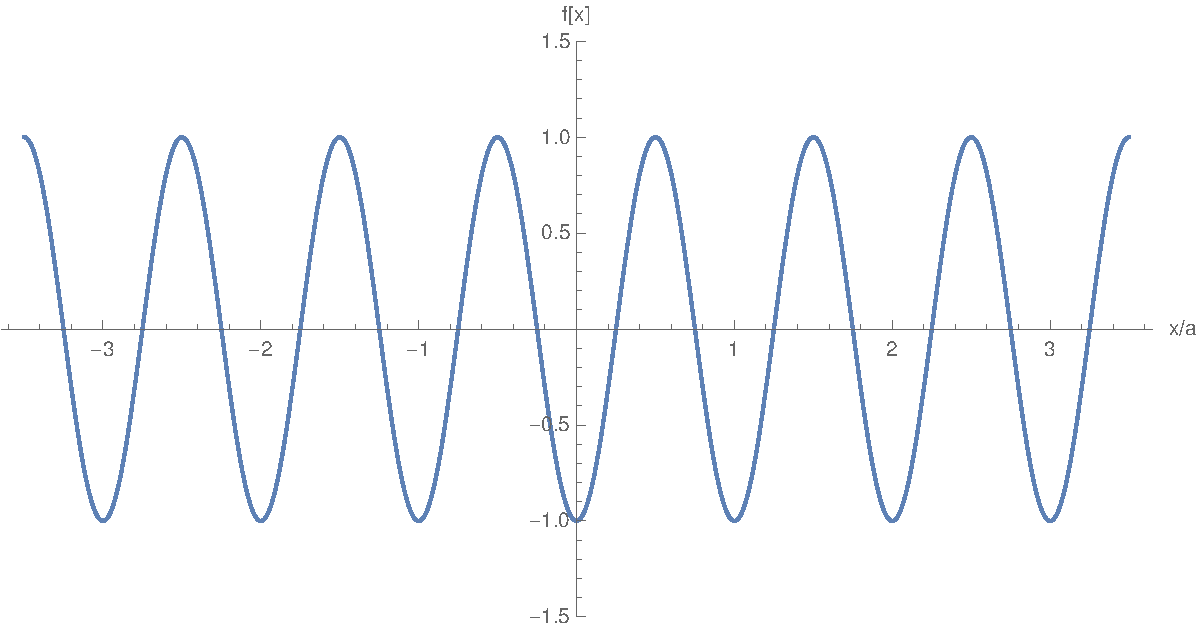
\includegraphics[width=1.0\textwidth]{intro/images/fPlot}
\end{center}
\end{figure}
In terms of its potential
energy due to other particles like itself, it might experience a hard core repulsion with an 
intermediate-range attraction/repulsion, such as the Lennard-Jones 
potential~\cite{atkins2011} shown in 
\begin{figure} \caption[The kind of interaction potential that might exist between two nearby particles.]{The kind of interaction potential that might exist between two nearby particles, $g(x)$. Here we have 
used a Lennard-Jones potential~\cite{atkins2011}, with parameters chosen so that the interaction scale is comparable to the
lattice spacing $a$. The particle generating this potential is located at the origin.} 
\label{fig:partInteraction}
\begin{center}
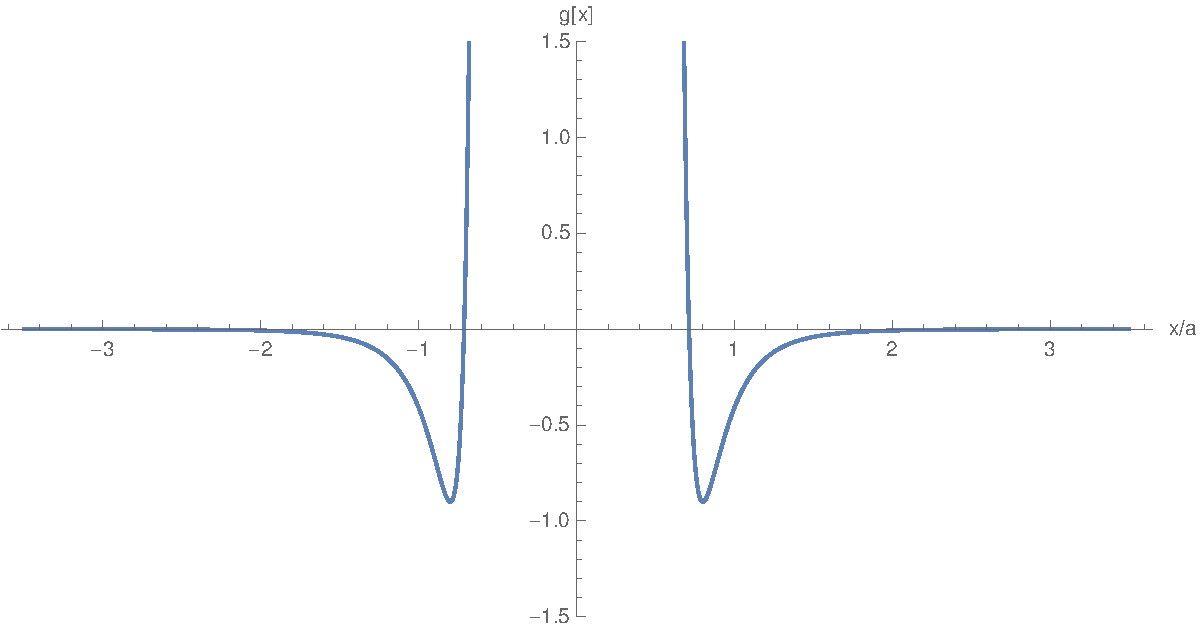
\includegraphics[width=1.0\textwidth]{intro/images/gPlot}
\end{center}
\end{figure}
Fig.~\ref{fig:partInteraction}. Thus, the 
total potential energy landscape from the particle's perspective might look something like 
Fig.~\ref{fig:fullPot}.
\begin{figure} \caption[The sum of the background and interaction potentials.]{The sum of the background
and interaction potentials, the interaction being generated by a particle at the origin. Notice that
the minimum closest to the origin has been greatly deepened, disproportionately to the lowering
of the peak between it and the next-nearest neighbour.} 
\label{fig:fullPot}
\begin{center}
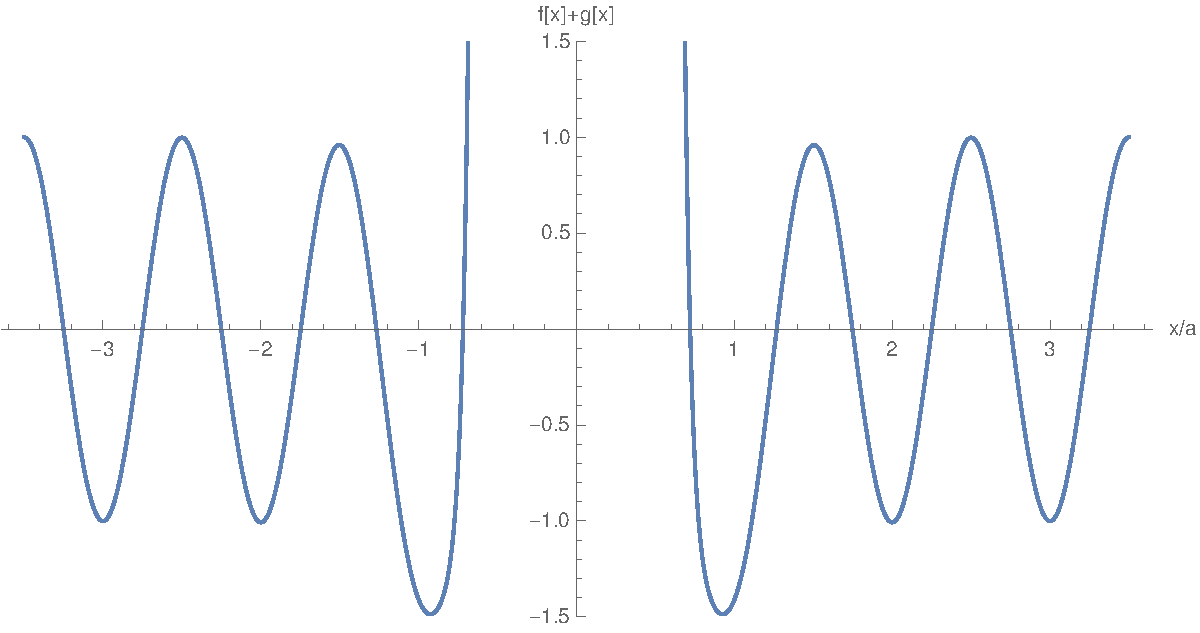
\includegraphics[width=1.0\textwidth]{intro/images/fgSumPlot}
\end{center}
\end{figure}
There are a few things to note here in terms of such a particle moving with
the influence of fluctuating forces:
\begin{enumerate}
\item Particles should be expected to spend the vast majority of their time in the minima of the 
externally-induced potential. This essentially creates a lattice of distinct slots within which a
particle
is highly likely to be at any given time. Thus it is reasonable to speak of particles occupying these 
``slots'' and occasionally transitioning between them.
 \item There is a large potential barrier opposing attempts by particles to get close together. Therefore,
 it is unlikely that multiple particles would be able to squeeze into the same slot,
 and so the assumption that each slot can contain at most one particle is a reasonable one.
 \item If the transition rates between adjacent slots behave in an Arrhenius-like manner~\cite{arrhenius1889, levine2005}, i.e.
 \begin{equation}
  \tau_0^{-1} \propto e^{\frac{\Delta U}{k_B T}},
 \end{equation}
 with $k_B T$ being the characteristic thermal energy,
then the rate of transition is dominated by $\Delta U$, the size of the ``energy barrier'' which
our particle must cross in order to escape from its slot and move to the next one. If we have a relatively
short-ranged intermediate component to the interparticle potential, we can see from Fig.~\ref{fig:fullPot}
that the dominant effect is on the depth of the potential well in which an adjacent particle sits, followed
by the height of the barrier the adjacent particle must cross in order to move away. As these
quantities are altered by different amounts on account of their different distances away from the particle
at the origin, we might expect that \textbf{the dominant affect of the presence of the original particle is
to alter the rate at which an adjacent particle will move away from it}. Of course, the depths and barrier
heights of other slots further away would also in general be affected, but if the interparticle interaction potential decays very rapidly over the length of a lattice spacing these next-neighbour effects will be
very small compared to the nearest-neighbour effect.
\item The particle and background lattice is also assumed to thermalize
after the hop. There 
should be no time-correlated "double hop" events or "two particle"
simultaneous hops.
\end{enumerate}

\subsection{The Sticky Particle Model}
Combining these ideas, we would do well to investigate models that exhibit exclusion (i.e. no more than one 
particle per slot), and in which particles hop away from adjacent particles 
differently to when they are on their 
own. Therefore, we propose a continuous-time Markov process with transition rates as indicated in
Fig.~\ref{fig:transRates}, which we call the Sticky Particle Model (SPM).
\begin{figure} \caption[The transition rates in the Sticky Particle Model.]{The transition rates in the Sticky Particle Model. Here white circles are particles, and black circles are vacancies. Dots indicate connections to the rest of 
the system; the configuration of the particles and vacancies there is irrelevant to the transition here due to the
interaction's short range. Arrows with accompanying quantities indicate possible transitions and their rates, here 
divided by the base rate $\tau_0^{-1}$.} 
\label{fig:transRates}
\begin{center}
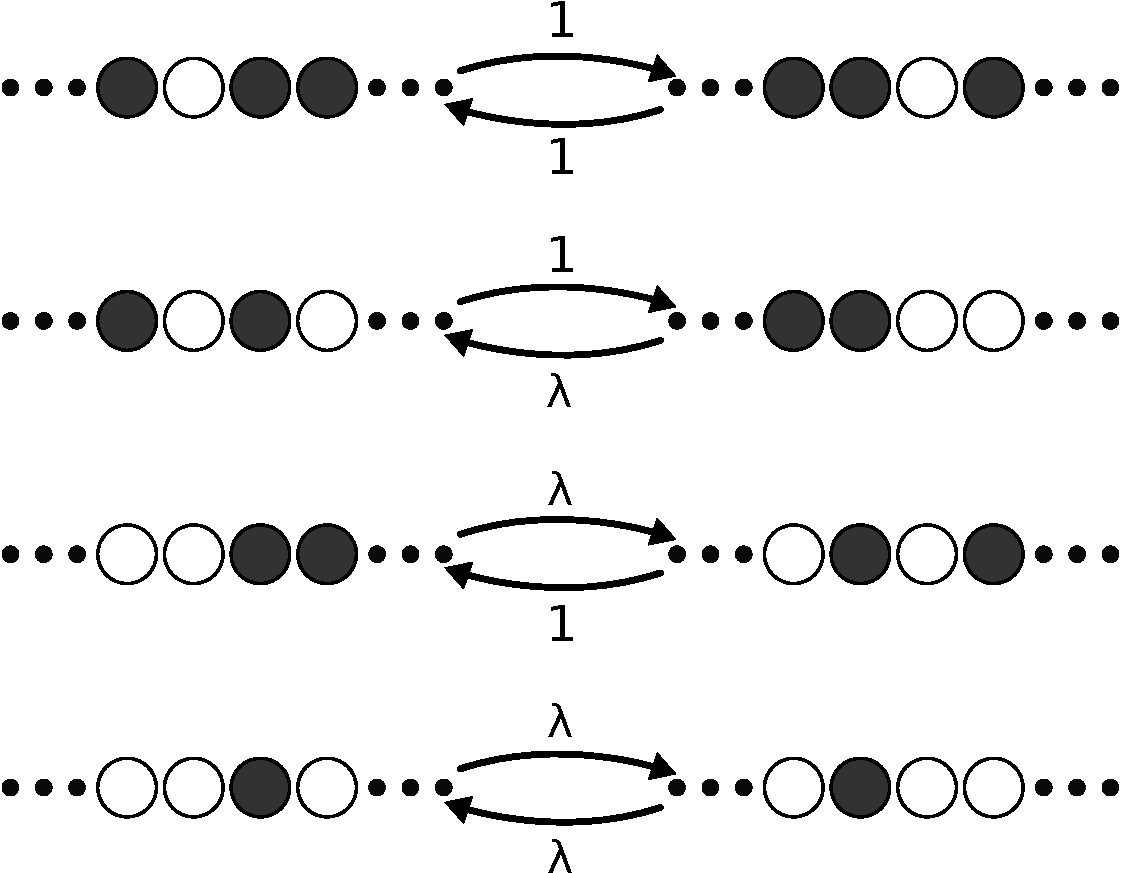
\includegraphics[width=1.0\textwidth]{intro/images/ratesDB}
\end{center}
\end{figure}
A simple verbal description of the model is as follows: particles move randomly into empty adjacent sites with rate 
$\tau_0^{-1}$, unless they are already adjacent to a particle, in which case they jump away from that adjacent
particle with rate $\lambda \tau_0^{-1}$. We have factored out $\tau_0$ because it is the ratio of these two rates,
$\lambda$, that is most important to the phenomenology of this model; rescaling $\tau_0$ is equivalent to 
rescaling time, which is in some sense trivial, whereas varying $\lambda$ should yield models with different behaviours.

Of course, this model is the epitome of a ``toy model'', and with good reason. The complexity of the
analysis of physical models generally scales quite unfavourably with the number of parameters; this model
has the benefit of having only one meaningful parameter, which should make it much easier for us
to explore model behaviour when we use numerical methods.

\section{Properties of the Sticky Particle Model} \label{sec:spmProperties}
Here we list a few properties that the SPM possesses. Note that these properties, although simple, are
often not shared by other models, and in some sense they mark the SPM out by its having all of them.
\subsection{Homogeneity}
The same transition rules apply to any particle in an SPM system regardless of spatial location.
We will break true homogeneity later on when we consider adding boundary conditions, but even then
we still have homogeneous dynamics in the bulk.
\subsection{Symmetry}
One of the more simple aspects of the SPM is its obvious mirror symmetry: that is, the system dynamics
are unchanged by a mirror symmetry transformation. This differentiates it from ASEP-like models~\cite{golinelli2006}; we
will say more about those in Sec.~\ref{sec:asep}. We will refer to this property as \textit{symmetry}.
\subsection{Locality}
The SPM has the property that a particle's transition rates are determined solely by its immediate
environment, in the sense that it can only hop into a space which is empty, and its rate of doing so
then only depends upon what is behind it. By taking account of what is behind it, the model is differentiated from SEP; by not accounting 
for anything further afield, it is not the
same as a more transparently energy-based model might be (although we will see that this model does
have an energy interpretation in Sec.~\ref{sec:dbProof}). We will henceforth refer to this property
as \textit{locality}.
\subsection{Detailed Balance} \label{sec:dbProof}
The SPM possesses the properties of homogeneity, symmetry and locality essentially by design. Indeed, it is
the only exclusion model in $1$D which possesses all of these
properties~\footnote{SEP also obeys these properties, but it is of course 
simply the $\lambda=1$ case of the SPM.}: a particle can only move into
an empty space (exclusion), and so then by locality we need only concern ourselves with its immediate 
neighbours to determine the hopping rate; then there are only two options, depending upon what is in the 
slot the particle is hopping away from, meaning that there are two possible rates, one for each occupation
of that neighbour. But by symmetry and homogeneity, these two rates must apply at every site, and equally
in both directions; thus, adopting all these properties gives us no choice but the SPM.

These rates also imply an additional property. Recall the definition of 
\textbf{detailed balance}~\cite{gardiner1985}:
that there exists
a probability distribution $P$ over configurations $\xi \in \Xi$ such that 
$\forall \xi_1 , \xi_2 \in \Xi $,
  \begin{equation} \label{eq:dbDefn}
    P(\xi_1) \cdot \sigma(\xi_1 \rightarrow \xi_2) = P(\xi_2) \cdot \sigma(\xi_2 \rightarrow \xi_1).
  \end{equation}  
Here, $\Xi$ is the space of all possible configurations for the SPM, and 
$\sigma(a \rightarrow b)$ is the transition rate from state $a$ to state $b$. In our case a transition
means performing one of the operations shown in Fig.~\ref{fig:transRates}. There,
we
list all of the motions that can occur, with all possible local environments: the central two slots must
contain exactly one particle and one vacancy in order for a transition to be possible, and there are two
ways to do this; then there are the two remaining slots at the sides, which can have any of the two
occupations each, so there are $8$ meaningfully different transitions in total.

Consider a probability distribution of the form $P(\xi) \propto \lambda^{-n}$, where $n$ is the total
number of particle-particle adjacencies in the system. In the outer two diagrams of 
Fig.~\ref{fig:transRates}, the forward and backward transition rates are identical, as are the number of
particle-particle adjacencies; thus Eq.~\eqref{eq:dbDefn} is trivially satisfied using the proposed 
distribution $P$. In the middle two diagrams, we see that reducing the number of adjacencies by one
occurs with rate $\lambda$, whilst increasing that number by one happens with rate $1$. Thus, in the 
language of Eq.~\eqref{eq:dbDefn},
\begin{equation}
 \lambda P_0 \cdot 1 = P_0 \cdot \lambda,
\end{equation}
where $P_0$ is a normalisation constant for the probability distribution. We see therefore that the SPM
transition rates satisfy the detailed balance condition with distribution $P$; we can interpret the 
detailed-balance energy as being located in the ``bond'' between two adjacent particles. In hindsight,
that the model obeys detailed balance is perhaps not so surprising; however, it is not immediately 
obvious from the transition rates alone.

An alert reader will have noticed that we still haven't discussed the domain on which the process takes 
place very much. In our detailed balance proof we used only the SPM bulk rates, 
so that this result only
applies to SPM systems defined on an infinite domain or on a finite ring. If one introduces boundaries,
and defines additional rates to define their behaviour, one will typically end up breaking detailed 
balance.

\section{Relationship to Existing Models} \label{sec:existingModels}
Of course, the SPM is not exactly ``new'': it is very similar to several models already discussed in the
literature. Here we will discuss the more prominent of these, with emphasis on why the SPM is different or
how we are going to analyse it differently to them.
\subsection{The Ising Model}
The SPM is equivalent to a constrained version of the classical Ising 
model~\cite{lenz1920, Ising1925, strecka2015} in $1$D; we can map SPM
occupations $\rho_i \in {0, 1}$ on to Ising spins $\sigma_i \in {-1, 1}$ via the transformation
\begin{equation}
 \sigma_i = 2 \rho_i - 1 .
\end{equation}
The constraint is that the magnetisation is locally conserved, i.e. we can only swap the spins of adjacent
sites during the dynamics. If we are careful with our definitions of the SPM transition rates,
the SPM is a equivalent to a method for numerically simulating the Ising model known as Kawasaki
dynamics, which has been in the literature for a long time~\cite{kawasaki1966, Garrido1990, grynberg2010}. 
Kawasaki dynamics was originally intended as
a stochastic Markov process designed to replicate the Ising model in equilibrium, albeit with a
constraint on the magnetisation, which makes more sense when the
dynamics are interpreted as a model of a two-species alloy. We have more 
to say about the correspondence with the Ising model in Sec.~\ref{sec:isingSim}.

In theory, one can calculate equilibrium properties of the SPM by using this equivalence to the constrained
Ising model; in order to do this, one may attempt to implement the constraint by varying the applied
magnetic field in such a way that the system ends up with the correct magnetisation, and then working
out desired quantities from there using the Ising partition function~\cite{baxter2016}. However, we found that
this results
in extremely convoluted algebra, and it is actually easier to build a new partition for the SPM from 
scratch, as we have done in Sec.~\ref{sec:spmPartFn}.
\subsection{SEP/ASEP/TASEP} \label{sec:asep}
The SPM also resembles the SEP/ASEP/TASEP family of models~\cite{liggett1985, golinelli2006, blythe2007,
Crampe2014}, 
as it is an
exclusion process. However, we 
have not found this resemblance to be particularly helpful, as these models do not contain the
nearest-neighbour interactions between particles that the SPM does. Thus, we do not believe that we are
able to solve the SPM using a similar matrix product solution to TASEP. Furthermore, ASEP and TASEP
are manifestly asymmetric in their bulk dynamics, whereas the SPM is not.

\subsection{The KLS Model}
The Katz-Lebowitz-Spohn (KLS) model~\cite{Katz1984, Zia2010} was originally designed to model the
behaviour of ions moving stochastically
under the influence of an external potential. The SPM is in fact a specific symmetric case of the
$1$-dimensional KLS model. Whilst the KLS model exhibits plenty of interesting behaviour
(in particular, the formation of stripes during flow in higher dimensions), most of the research done
into it has involved using asymmetric versions of the model to drive flow. The stationary
distribution for the symmetric version on a ring is given in~\cite{Katz1984}, whilst the version with open boundaries
which we study here has received far less attention.

\section{Research Outline}
Our investigation into the SPM has focussed primarily upon its flow characteristics when driven
by concentration gradients imposed by boundary conditions. This does not seem to have been something
which has been investigated much before; as we have hinted in Sec.~\ref{sec:existingModels}, most
research into flow in many-body systems uses internal dynamics to drive the flow instead of the 
boundaries. Therefore, we are essentially working from scratch with this model.
To present our results, we are using the following structure:
\begin{itemize}
 \item We use primarily analytic methods in Ch.~\ref{sec:analChap}. These include the evaluation
 of the partition function for the SPM on a closed ring (Sec.~\ref{sec:spmPartFn}), the development
 of the mean-field theory of the SPM (Sec.~\ref{sec:spmMft}) and its generalisation to higher dimensions
 (Sec.~\ref{sec:highDimSPM}).
 \item In Ch.~\ref{sec:transRateChapter} we introduce a method for using sparse numerical linear
 algebra to exactly solve the steady state distribution for small $1$D SPM systems. We also show how this
 method can be used to compute some time-dependent quantities in Sec.~\ref{sec:TRMTimeDep}.
 \item In Ch.~\ref{sec:numerics} we discuss the use of Monte-Carlo methods to calculate the properties
 of the SPM in somewhat larger $1$D and $2$D systems. In particular we focus on the Kinetic
  Monte-Carlo algorithm (KMC) in Sec.~\ref{sec:nFoldWay}, and calculate the bulk of our results
  using it.
\item We summarise our main conclusions in Ch.~\ref{sec:conclusionsChap}.
\end{itemize}


% mention Ising and ASEP

\chapter{Analytical Results about the SPM}

\section{Existing Approaches to Nonequlibrium Statistical Mechanics}
\subsection{Mean-Field Theory}
Quick history of this, how to use it, when it might work.
\subsection{Exact Solutions}
Talk about stuff like ASEP. Remember to mention that only very specific models seem to be analytically solveable, in particular you can't have interactions and range in the current models.
\subsection{Where does the SPM stand?}
Basically, why we can't analytically solve it, and so why performing mean-field approximation is a decent start.

\section{Analytic Derivations from the SPM in 1D}
This stuff is kinda self-explanatory.
\subsection{Lattice MFT Derivation}
\subsection{Continuum Limit MFT Derivation}
\subsection{Negative Diffusion Coefficients}
When do they happen? What do they mean?
\subsection{Continuum Limit MFT Solutions}
There's a bunch of these.
\subsection{Continuum MFT Breakdown}

\section{The SPM in Higher Dimensions}
Kinda repeat the earlier stuff in higher dimensions, particularly 2 where we actually have data. Maybe less need for elaborate sections structure here; just write freely and see how it goes.


%\chapter{Transition Rate Matrix Analysis} 
\label{sec:transRateChapter}
Now that we have MFT predictions about the relationship between density difference and
current in the SPM, it would be good to try to investigate their validity. In Chapter~\ref{sec:numerics} we will use Monte-Carlo methods to do this in $1$d and $2$d, but in this chapter we will restrict our attention to $1$d.

\section{The Transition Rate Operator for the SPM} \label{sec:TRMGeneralResults}
The SPM is an autonomous continuous-time Markov Process, which describes continual transitions between states
with transition rates depending only upon the current state. As such, if we call the total space of
states $\Xi$ then the probability distribution $P: \Xi \times \mathbb{R} \rightarrow  \mathbb{R}$ should obey a \textbf{master equation}
\begin{equation} \label{eq:masterEq}
 \partDeriv{P(\xi, t)}{t} = \mathcal{A} P(\xi, t),
\end{equation}
where $\mathcal{A}:\Xi \rightarrow \Xi$ is the \textbf{transition rate operator}
or TRO. Note that I am going to be using column vectors for probabilities rather than
row vectors, as many in the probability community do.
Parametrising $\mathcal{A}$ via 
\begin{equation}
 (\mathcal{A}f)(u) = \int_\Xi \! \! \mathrm{d}  \xi \ \sigma (u, \xi) f(\xi)
\end{equation}
puts it in a more familiar, transport equation-style notation:
\begin{equation}
 \partDeriv{P(\xi, t)}{t} = \int_\Xi \! \! \mathrm{d}  u \ \sigma (\xi, u) P(u, t) .
\end{equation}
Here $f: \Xi \rightarrow \mathbb{R}$ is an arbitrary function, intended to be a probability
distribution (nonnegative, unit measure, etc), whilst $\xi , u \in \Xi$ are dummy variables
and $\sigma: \Xi \times \Xi \rightarrow \mathbb{R}$ represents $\mathcal{A}$ in the basis 
determined by how we perform the integration.

We demand that $\sigma$ satisfies
\begin{equation}
 \forall \xi \in \Xi, \ \sigma (\xi , \xi) \le 0 
\end{equation}
and
\begin{equation}
 \forall \xi_1 , \xi_2 \in \Xi : \xi_1 \ne \xi_2 , \ \sigma (\xi_1 , \xi_2) \ge 0 ,
\end{equation}
as well as the constraint
\begin{equation}
 \forall u \in \Xi , \ \int_\Xi \! \! \mathrm{d}  \xi \ \sigma (\xi, u) = 0.
\end{equation}
The last constraint implies that
\begin{equation}
 \int_\Xi \! \! \mathrm{d}  \xi \partDeriv{P(\xi, t)}{t} = \int_\Xi \! \! \mathrm{d}  u \ P(u, t) \left[ \int_\Xi \! \! \mathrm{d}  \xi \ \sigma (\xi, u) \right] = 0
\end{equation}
regardless of the structure of $P$, which is our probability conservation equation.

The formal (forward-time) solution to Eq.~\eqref{eq:masterEq} is given by
\begin{equation} \label{eqn:formalSoln}
 P(\xi, t) = e^{(t-t_0)\mathcal{A}}P_0,
\end{equation}
where $t_0$ is some initial time, $P_0$ is the starting distribution, and the operator
exponential is defined by its Taylor expansion, which should converge fine for bounded
$\mathcal{A}$, satisfied for the finite-system SPM. As 
$e^{(t-t_0)\mathcal{A}}$ and $\mathcal{A}$ share eigenvectors, we see that the
eigenstructure of $\mathcal{A}$ is something well worth investigating, as it should
give us information about the time-evolution of the system. An important thing to point
out is that $\mathcal{A}$ does not in general have orthogonal eigenvectors because it is
not in general symmetric,
and so we cannot normally diagonalise it using orthogonal transformations. This means that modes do not ``decouple'' in the way that states do in the 
Schr\"{o}dinger equation, and we instead have to deal with an \textbf{adjoint system}~\cite{stoll2008}.

Luckily, when it comes to the analysis of steady states, there are a few results that
can help us. If we consider the operator $\mathcal{G}_T = e^{T\mathcal{A}}$ (in other words, the 
\textbf{propagator} for a period of time $T$), it is pretty easy to see that this is
a standard Markov Operator, as we are essentially reversing the limiting process
we would perform in order to define a continuous time Markov process as a limit of
a discrete time one. If we assume that $\Xi$ is finite and $\mathcal{G}_T$ is irreducible then as
a Markov operator it must possess  a unique eigenvector with corresponding eigenvalue $1$.
All other eigenvalues must have modulus between $0$ and $1$. Therefore, $\mathcal{A}$
must share that same unique eigenvector with associated eigenvalue $0$, and its other
eigenvectors must have negative real part. In physical terms, the system must have a single
steady state probability distribution, which it always relaxes towards exponentially
quickly, with a rate determined by the nonzero eigenvalue of $\mathcal{A}$ with real
part closest to $0$.

Of course, for such finite-state systems (such as the SPM on a finite domain) the integrals become sums, and $\sigma$ a matrix, $Q$. In such systems, we can arrange to have some labelling scheme which uniquely relates system states to natural numbers, and therefore
relates states to basis vectors in a vector space. In the SPM, a site is either full or empty, which means that there is a natural mapping between states and natural numbers based upon binary representation;
a string of $1$s and $0$s can be associated with a natural number as well as a configuration of particles and vacancies.

\subsection{A Small Worked Example: Closed System} \label{sec:workedExampleClosed}

As a concrete example, let us consider the SPM on a cyclic domain of length $3$. There
are $2^3$ possible combinations, and so $8$ possible states: $000$, $001$, and so forth.
The transition rate matrix describing this system is:
\begin{equation}
 Q =
 \begin{bmatrix}
0  &   &   &           &   &   &   &   \\
   &-2 & 1 &           & 1 &   &   &   \\
   & 1 &-2 &           & 1 &   &   &   \\
   &   &   & -2\lambda &   &  \lambda &  \lambda &   \\
   & 1 & 1 &           & -2&   &   &   \\
   &   &   &  \lambda    &   &  -2\lambda & \lambda  &   \\
   &   &   &  \lambda  &    & \lambda  & -2 \lambda &   \\
   &   &   &           &   &   &   & 0  \\
\end{bmatrix},
\end{equation}
where we have omitted most of the zero entries for clarity.
An alert observer will note that $Q$ is reducible, and so by permuting the basis vectors
we can rearrange the matrix into block form:
\begin{equation}
 Q ' = 
 \begin{bmatrix}
-2  & 1 & 1 &           &   &   &   &   \\
 1 &-2 & 1 &           &  &   &   &   \\
 1 & 1 &-2 &           &  &   &   &   \\
   &   &   & -2\lambda & \lambda &  \lambda &   &    \\
   &   &   &      \lambda& -2\lambda   &  \lambda &   \\
   &   &   &  \lambda   &   -2\lambda & \lambda & &   \\
   &   &   &       &  &  & 0 &  \\
   &   &   &           &   &   &   & 0  \\
\end{bmatrix}.
\end{equation}

According to our recipe, to learn about the solutions to Eq.~\eqref{eq:masterEq} 
in this case, we need to know about the eigendecomposition of $Q$. 
The block structure of $Q'$ means that there are $4$ 
distinct parts of the state space, between which there are no transitions; this 
partitioning corresponds to the fact that particle number is conserved on the ring.
Two of these
sectors correspond to the full and empty states, and their dynamics are completely
trivial, in the sense that the state space is $1$d and there are no dynamics, as the
particles/vacancies have nowhere to go.
The remaining sectors correspond to the situation where there is one particle or one 
vacancy. The matrix is symmetric, meaning that its eigenvalues are real,
and we find that both nontrivial blocks can be diagonalised to form a multiple of
\begin{equation}
 \begin{bmatrix}
  0  &  &  \\
     &-3&  \\
     &  &-3\\
 \end{bmatrix},
\end{equation}
with eigenvectors $[1, 1, 1]^{\mathrm{T}}$, $[-1, 0, 1]^{\mathrm{T}}$ and
$[-1, 1, 0]^{\mathrm{T}}$ respectively, the latter two forming a degenerate eigenspace.

In this particular example then, we find that there $4$ steady states:
\begin{itemize}
 \item All slots full,
 \item All slots empty,
 \item One particle present, with equal chance to be in any particular position,
 \item The same but with a vacancy instead of a particle.
\end{itemize}
Whilst the first 2 cases are trivial (one-dimensional probability spaces), in the other
two cases we relax towards the steady state with rates $3$ and $3\lambda$ respectively.
In this example, the TRM was actually symmetric, and so all the eigenvalues were real.
It was also highly reducible, due to the strict constraints imposed by the particle
conservation law. When we have boundary conditions which permit the creation and
destruction of particles, that will change; we will consider that situation now.

\section{Forming the TRM for Systems with Dirichlet Boundary Conditions}

\subsection{Dirichlet Boundary Conditions} \label{sec:CTMPBoundaries}
In Ch.~\ref{sec:analChap} we made an MFT for the SPM in $1$-dimension, and when 
investigating steady states used Dirichlet boundary conditions when we needed them.
In particular, we had a system of length $L$ and sought solutions in which the system
density was pinned at $\rho_0$ at $x=0$ and $\rho_L$ at $x=L$. 

We would like to do a similar thing for the non-MFT SPM. An exact analogue of the situation
does not exist, as occupation number is not defined \textit{a priori} in a Markov process, but merely emerges as a result of the rates prescribed. The closest imitation to it
we can get is by allowing particles to be created and destroyed in boundary regions at
either end of a chain, and then try to set these rates so that the time-averaged occupation probability in the end sites are $\rho_0$ and $\rho_L$ respectively. Note
that this is a little more involved than simply loading and unloading particles as
one does in ASEP, as
\begin{itemize}
 \item loading and unloading really doesn't simulate the boundary condition we are looking for,
 which is attachment to a particle reservoir of constant particle density, and
 \item we actually need to consider a two-site boundary layer attached to each end, because the internal dynamics of the particles depend upon their immediate environment.
\end{itemize}
To simulate a boundary which is attached to a reservoir with occupation $\rho$, we allow
particles to appear in empty boundary sites with rate $B_0 \sqrt{\frac{\rho}{1-\rho}}$
and to disappear from full ones with rate $B_0 \sqrt{\frac{1-\rho}{\rho}}$,
for some positive $B_0$. If we switch
off all other dynamics and consider this in isolation, we would have a collection of
decoupled two-state systems. Writing a TRM for this with the first basis vector being
the empty state and the second the full one, we get
\begin{equation} \label{eq:blinkRates}
 Q = 
 \begin{bmatrix}
  - B_0 \sqrt{\frac{\rho}{1-\rho}} & B_0 \sqrt{\frac{1-\rho}{\rho}} \\
  B_0 \sqrt{\frac{\rho}{1-\rho}} & -B_0 \sqrt{\frac{1-\rho}{\rho}} \\
 \end{bmatrix}.
\end{equation}
There is of course a zero eigenvalue, which corresponds to a stationary distribution
$ [1-\rho, \rho]^\mathrm{T} $, precisely as desired.

In order to simulate attaching a reservoir with particle density $\rho$, we apply
the creation and annihilation rates above to the outermost two sites in our lattice.
The outermost site only performs these operations. The inner boundary site undergoes
these creation and annihilation processes, as well as the normal dynamics of the SPM;
thus, particles will move in and out of it as normal, and when the outermost site's
occupation is required to determine the transition rate for a particle moving inward,
that information is available. One could possibly eliminate the need for the outermost
boundary site by averaging over occupations, however we have chosen not to do this for
consistency with our Monte-Carlo calculations in Ch.~\ref{sec:numerics}.

Observant readers will notice that by using these creation and annihilation rates we
are left with a free variable, $B_0$. This controls the ratio of the creation and
annihilation rates to the internal dynamical rates $1$ and $\lambda$. In general
when we're trying to simulate an adjacent reservoir we want the boundary motion to be
``fast'' compared to the internal dynamics, and so $B_0$ may be regarded as a
regularisation parameter; any choice of $B_0$ should be good so long as
the creation and annihilation rates sufficiently dominate both $1$ and $\lambda$.
In practise, in our larger-scale calculations we  used
\begin{equation}
 B_0 = b(1+\lambda),
\end{equation}
with $b$ set to, $100$ or $1000$.

\subsection{Another Small Worked Example: Open System}

Using full boundary conditions, the smallest system we can consider consists of adjacent boundary
layers, in which particles pass directly from the inner layer of one boundary to the inner layer
of the other boundary. Unfortunately the state space of such a system is $2^4=16$-dimensional, and
so it would be cumbersome to consider such a system as an example here.

However, in the special case in which one boundary has density $\rho_0=1$ and the other has
$\rho_L=0$, the outer boundary layers become nondynamical, and the system simplifies considerably;
particles can only enter at the full end with rate $\lambda$, and can only leave at the empty end.
Therefore, we can consider a system consisting of single boundary layers attached to a single internal
slot without needing to consider a state space larger than $2^3=8$. Using the same state-labelling
convention as in Sec.~\ref{sec:workedExampleClosed}, the TRM for this new open system is
\begin{equation}
Q = 
\begin{bmatrix}
 -\lambda  & 1 &   &   &   &   &   &   \\
   & -\lambda -2 & 1 &   &   &   &   &   \\
   & 1 & -\lambda -2 & 1 & \lambda  &   &   &   \\
   &   &   & -2 \lambda -1 &   & \lambda  &   &   \\
 \lambda  &   & 1 &   & -\lambda  & 1 &   &   \\
   & \lambda  &   & \lambda  &   & -\lambda -2 & \lambda  &   \\
   &   & \lambda  &   &   & 1 & -\lambda  & \lambda  \\
   &   &   & \lambda  &   &   &   & -\lambda  \\
\end{bmatrix}.
\end{equation}
This time the matrix is not symmetric, and there does not exist a basis permutation which puts the
TRM into block form. If we calculate the characteristic polynomial $p(q) = |Q - q I|$, we find that
\begin{equation}
\begin{split}
 &p(q) = q \left[ q^7+(9 \lambda +7) q^6+\left(34 \lambda ^2+53 \lambda +17\right) q^5+\left(71 \lambda ^3+165 \lambda ^2+103 \lambda +17\right) q^4+ \right. \\
 &+\left(89 \lambda
   ^4+274 \lambda ^3+247 \lambda ^2+76 \lambda +6\right) q^3+\left(67 \lambda ^5+256 \lambda ^4+294 \lambda ^3+126 \lambda ^2+17 \lambda \right) q^2 \\
  &\left. +\left(28 \lambda ^6+127 \lambda ^5+171 \lambda ^4+91 \lambda ^3+15
   \lambda ^2\right) q + \left(5 \lambda ^7+26 \lambda ^6+37 \lambda ^5+24 \lambda ^4+4 \lambda ^3 \right) \right].
\end{split}
\end{equation}
Of course, the roots of $p(q)$ are the eigenvalues of $Q$. Clearly one of the eigenvalues is $q=0$,
and the others could be found by finding the root of the $7^\mathrm{th}$ order polynomial, which we
will not be doing analytically because it is extremely tedious and besides the point of this
example. The
$0$-eigenvector, and therefore the steady-state probability distribution over the possible
configurations, can be computed with a little care, and turns out to be
\begin{equation}
 q_0 = D^{-1}
 \begin{bmatrix}
  3 \lambda +1,\lambda  (3 \lambda +1) \\
  \lambda  (\lambda +2) (3 \lambda +1) \\
  \lambda ^3 (\lambda +3) \\
  (\lambda +3) (2 \lambda  (\lambda +2)+1) \\
  \lambda ^2 (\lambda +3) (2 \lambda +1) \\
  \lambda  (\lambda  (\lambda (\lambda +8)+14)+5) \\
  \lambda ^3 (\lambda +3) \\
 \end{bmatrix},
\end{equation}
where
\begin{equation}
 D = \lambda  \left[\lambda  (\lambda  \left[5 \lambda +26\right]+37)+24 \right]+4.
\end{equation}
The variation of the occupation probabilities with $\lambda$ is displayed in
Fig.~\ref{fig:smallOccProbs}.
 \begin{figure}[h!]
 \caption[The variation of configuration probabilities with $\lambda$ for a small open system.]{\label{fig:smallOccProbs} 
 The variation of the steady-state configuration probability distribution with $\lambda$ for our
 open system. The coloured curves correspond to specific configurations, as indicated in the legend.
 }
  \begin{center}
 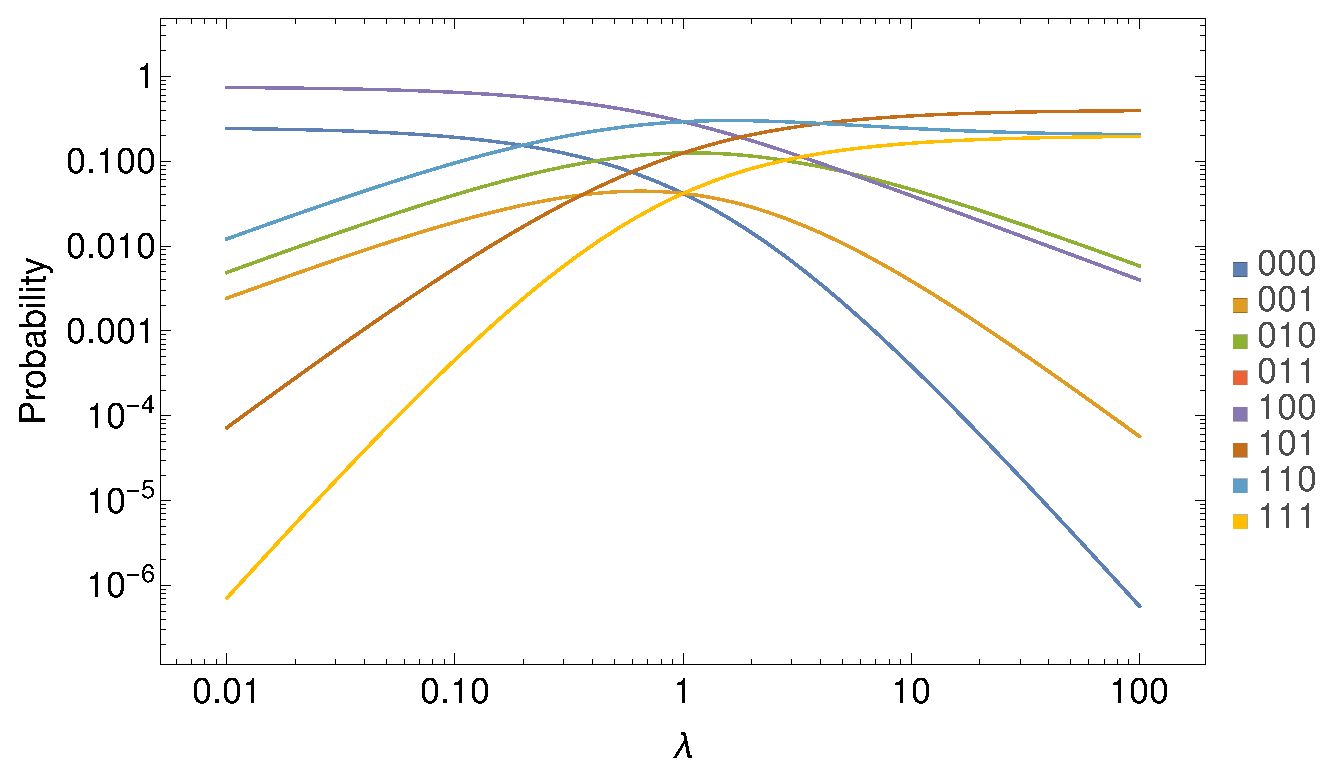
\includegraphics[width=1.0\textwidth]{TRM/images/smallOpenOcc}
  \end{center}
\end{figure}
Notice that at extremely small $\lambda$ the system either empties or a single particle gets stuck to
the full boundary, 
essentially preventing further flow by blocking it. Meanwhile, at large $\lambda$ there are
a few fairly popular states, the most dominant being one with alternating particles and 
vacancies, as one might expect. The steady-state current from left to right in this system can be
calculated analytically once we have the steady state probability distribution, and turns out to be
\begin{equation}
 J = \lambda \left[ \frac{1}{4} + \frac{(1-\lambda)(3+\lambda)\lambda^2}{4+
 \lambda\left(24+\lambda\left[37+\lambda\left(26+5\right)\right]\right)}  \right].
\end{equation}
The second term in the bracket is generally dominated by the first, so we can say to an excellent
approximation that $J \sim \frac{1}{4} \lambda$. Thus, at least for this tiny example with very
extreme boundary conditions, there does not appear to be any change in the scaling of the current
with $\lambda$.

We can also compute the negative real part of the eigenspectrum of the TRM for this small system;
this is displayed in Fig.~\ref{fig:smallEigSpec}.
 \begin{figure}[h!]
 \caption[The variation of the eigenspectrum of the TRM with $\lambda$ for a small open system.]{\label{fig:smallEigSpec} 
 The variation of the negative real part of the eigenspectrum of the TRM for our small open system
 with $\lambda$.
 }
  \begin{center}
 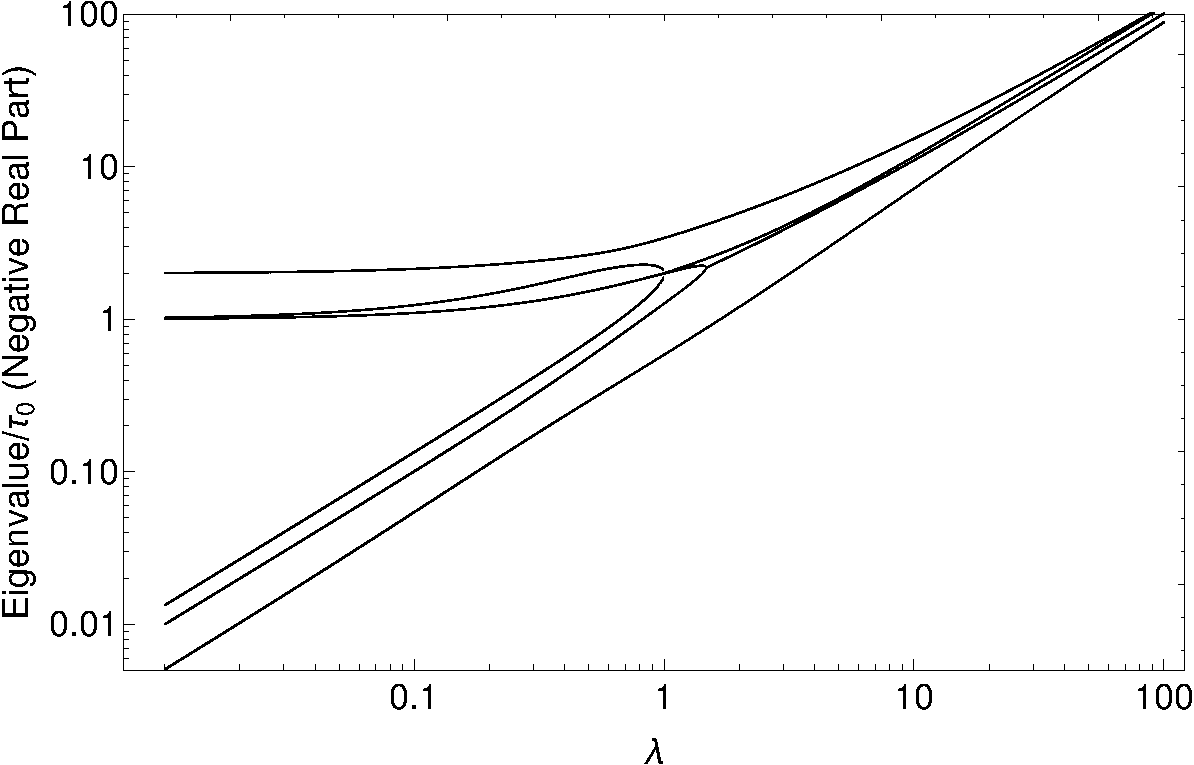
\includegraphics[width=1.0\textwidth]{TRM/images/smallOpenEigSpec}
  \end{center}
\end{figure}
It is in many ways rather similar to the eigenspectra we find for larger systems, so see Sec.~\ref{sec:trmEigenspec} for our comments on those.

\subsection{Construction of the TRM in Sparse Format}

As we have seen, it is possible to find the eigendecomposition of the TRM analytically for extremely
small systems with special boundary conditions. However, we'd really like to see what happens for
somewhat larger systems, with more diverse boundary conditions. Thus, let us try to develop
a method for the numerical analysis of TRMs of arbitrary size.

The important thing to note about transition rate matrices for local lattice models
such as the SPM is that whilst the TRM itself grows very aggressively with system size, the TRM is generally extremely sparse.
The state space dimension grows as $2^L$, and the TRM dimension therefore grows as
$2^L \times 2^L$. However, a state containing $N$ particles only has transitions to
\begin{itemize}
 \item states which differ from the current state by one particle move, of which there
 are $\mathcal{O}(N)$, and
 \item states which differ from the current state by a single particle creation or
 annihilation, of which there are $\mathcal{O}(4)$.
\end{itemize}
Thus, as $N \le L$ the number of nonzero entries in the matrix is 
$\mathcal{O}(2^{L}L)$,
which is not a particularly tight bound. Therefore, the overall density of the TRM
is $\mathcal{O}(2^{-L}L)$. Given that there already exist a great many efficient
numerical routines for sparse linear algebra operations, there exists the possibility
that we could use this to solve the SPM on a finite domain for small systems
``exactly'' (or at least, up to some nominated numerical tolerance).

To make use of this, we need to assemble the TRM in a suitable sparse format.
I have written a Python code which does this. The script itself may be 
found in~\cite{hellier2019b} at 
\texttt{codes/exact/matStuff/sparseSysRep.py}, but the gist of the algorithm is to simply run through all possible states,
document all the transitions they can perform, and store the resulting entries in
a sparse matrix element by element. During construction, the matrix should be stored in
coordinate list format, i.e. a list of elements of the form $(\mathrm{row}, 
\mathrm{column}, \mathrm{value})$, as this is trivial to update as we only inspect
each matrix entry once. We can then convert the matrix to a compressed format such
as CSC (\textbf{Compressed Sparse Column}) or CSR
(\textbf{Compressed Sparse Row}). We used CSC, but in
hindsight CSR would probably have been a better choice as it tends to make
matrix-vector multiplication a little more efficient. Once we have the TRM in this
format, it is ready for sparse linear algebra operations. Note that whilst
these operations generally happen ``in place'', this part of the process is the
memory-intensive bit, as of course the memory usage scales with the number of nonzero
matrix elements, which is $\mathcal{O}(2^{L}L)$.
In terms of actual numbers, we found
that 4Gb of memory was more than adequate to solve a system of $16$ sites in total.
As the memory required to represent the TRM is the main limiting factor in this kind of
calculation, if we were to attempt a larger calculation we would probably switch to using a
machine with a very large working memory, such as DiRAC.

\section{The Eigenspectrum of the TRM}

\subsection{The Computation of the TRM Eigenspectrum} \label{sec:eigenFind}
Once we have the TRM $Q$ in CSC or CSR format, we can then use sparse linear algebra. 
In our code we called the Python routine \texttt{scipy.sparse.linalg.eigs} upon it,
which itself is a wrapper for C codes~\cite{lehoucq1998} which find eigenpairs according to desired
criteria; precisely which algorithm to used is determined during runtime, and it may
try different methods if it doesn't initially succeed.

In our computations, we typically performed two types of calculation. In the first we merely sought to
find the steady state, so which we requested only the eigenvector $x_0$
associated to the
eigenvalue $q_0$ with smallest absolute value, which should always be numerically zero.
We requested that the eigenpair be found to a relative accuracy $\epsilon$ accuracy of $1$ part in $10^{12}$,
which amounts to saying that
\begin{equation} \label{eq:linAlgRelAcc}
 \frac{\| Q x_0 - q_0 x_0 \|}{\| x_0 \|} \le 10^{-12} = \epsilon
\end{equation}
where $\| \cdot \|$ is some reasonable subordinate matrix norm (in our case, the $1$ norm). Because we requested the eigenvalue closest to $0$, \texttt{eigs} used the
shift-invert method~\cite{panju2011}, 
leading to greater accuracy in the computation of
eigenvalues near to $0$ which is exactly what we wanted. For the other type of
computation, we instead requested the $k$ eigenpairs with largest real part, which
most likely provoked the code to use a Implicitly Restarted Arnoldi Method (IRAM)~\cite{lehoucq1996, lehoucq1999}.
This is not as accurate for computing the steady state, but yields vastly more accurate
results when computing the other eigenpairs compared to the first method. 

\subsection{The Structure of the TRM Eigenspectrum} \label{sec:trmEigenspec}

Using our code (\texttt{codes/exact/matStuff/sparseSysRep.py} 
in~\cite{hellier2019b}), 
we can compute the eigenspectrum of an SPM system
with boundary densities connected at both ends. Such a computation requires the
following parameters to be specified:
\begin{itemize}
 \item $\rho_0 \in (0, 1)$, the density of the reservoir connected to the left end of the domain.
 \item $\rho_L \in (0, 1)$, the density of the reservoir connected to the right end of the domain.
 \item $L \in \mathbb{N}$, the system size.  The way we have defined things in the code, we do not
 count the two sets of two particles representing the boundary; thus, $L=1$ actually
 refers to a system which contains $5$ lattice sites, of which $4$ are busy doing
 boundary duties.
 \item $b>0$, the variable which controls the separation of timescales between the 
 flickering motion on the boundaries and the internal motion within the bulk of the
 system. This should be set to something large, and compared to other values of it
 to ensure that it is working as a regularisation parameter
 (i.e. large changes to $b$ have minimal impact on the relevant internal
 dynamics of the system, even if they have a great impact on the boundary dynamics).
 \item $\lambda>0$, the internal anomalous movement rate in the SPM.
 \item $\epsilon$, the relative accuracy the calculation aims for in the sense of Eq.~\eqref{eq:linAlgRelAcc}.
 \item $1 \le k < 2^{L+4}$, the number of eigenvalues to compute.
 \end{itemize}

 For consistency we kept $L$, $b$, $\epsilon$ and $k$ constant during runs of 
 calculations. This leaves $\rho_0$, $\rho_L$ and $\lambda$ to be varied. In terms of what to vary and how to display the data, we decided to
 allow the spectrum to depend upon only one variable, and picked $\lambda$ to be that
 variable. We generally chose $\rho_0 =0.6$ and $\rho_L =0.4$ in order to study a system in which,
 at least for $\lambda=1$, the density is middling and a current flows.
 We then computed the resulting eigenspectrum in a couple different ways.
 First, we performed a relatively small calculation, in terms of the number of eigenvalues demanded and the number of $\lambda$ used. We altered the values of $L$
 and $b$ between runs, so that we can see what impact they have on the eigenspectrum. We then performed a very
 large calculation, in order to get a good look at the eigenstructure as a whole.
 In Ch.~\ref{sec:analChap} our MFT suggested that a transition might occur around
 $\lambda=\frac{1}{4}$, so we should look out for odd behaviour in that regime.

 To actually perform these TRM calculations, we used Edinburgh Compute and Data Facility's Linux
 Compute Cluster, known as Eddie3. We will discuss this machine and its capabilities further in
 Chapter~\ref{sec:numerics}. Although we did initially consider the possibility of exploiting the natural parallelisability of the numerical linear algebra routines, we concluded that it
 was not probably not worthwhile in terms of computational gains, whilst requiring a lot of
 extra development time to implement. Instead, we simply submitted large numbers of separate serial
 jobs with different parameter values (e.g. for $\lambda$, $\rho_0$, $\rho_L$) to Eddie3, and then
 allowed the machine to process them in its own time.
 
 \subsubsection{Small Calculations}
 First, we performed a calculation with $L=5$, $b=1000$ in which we computed the
 negative real part of the $32$ eigenvalues with real part closest to zero for a wide range of $\lambda$ with fixed
 boundary conditions. The resulting eigenspectrum is displayed in
 Fig.~\ref{fig:eigsL5B1000}.
 \afterpage{
 \begin{figure}[!ht]
 \caption[The TRM eigenspectrum for a system with $L=5$, $b=1000$.]{\label{fig:eigsL5B1000} 
 The TRM eigenspectrum, computed for a system with $\rho_0 = 0.6$, $\rho_L = 0.4$,
 $L=5$, $b=1000$.
 }
  \begin{center}
 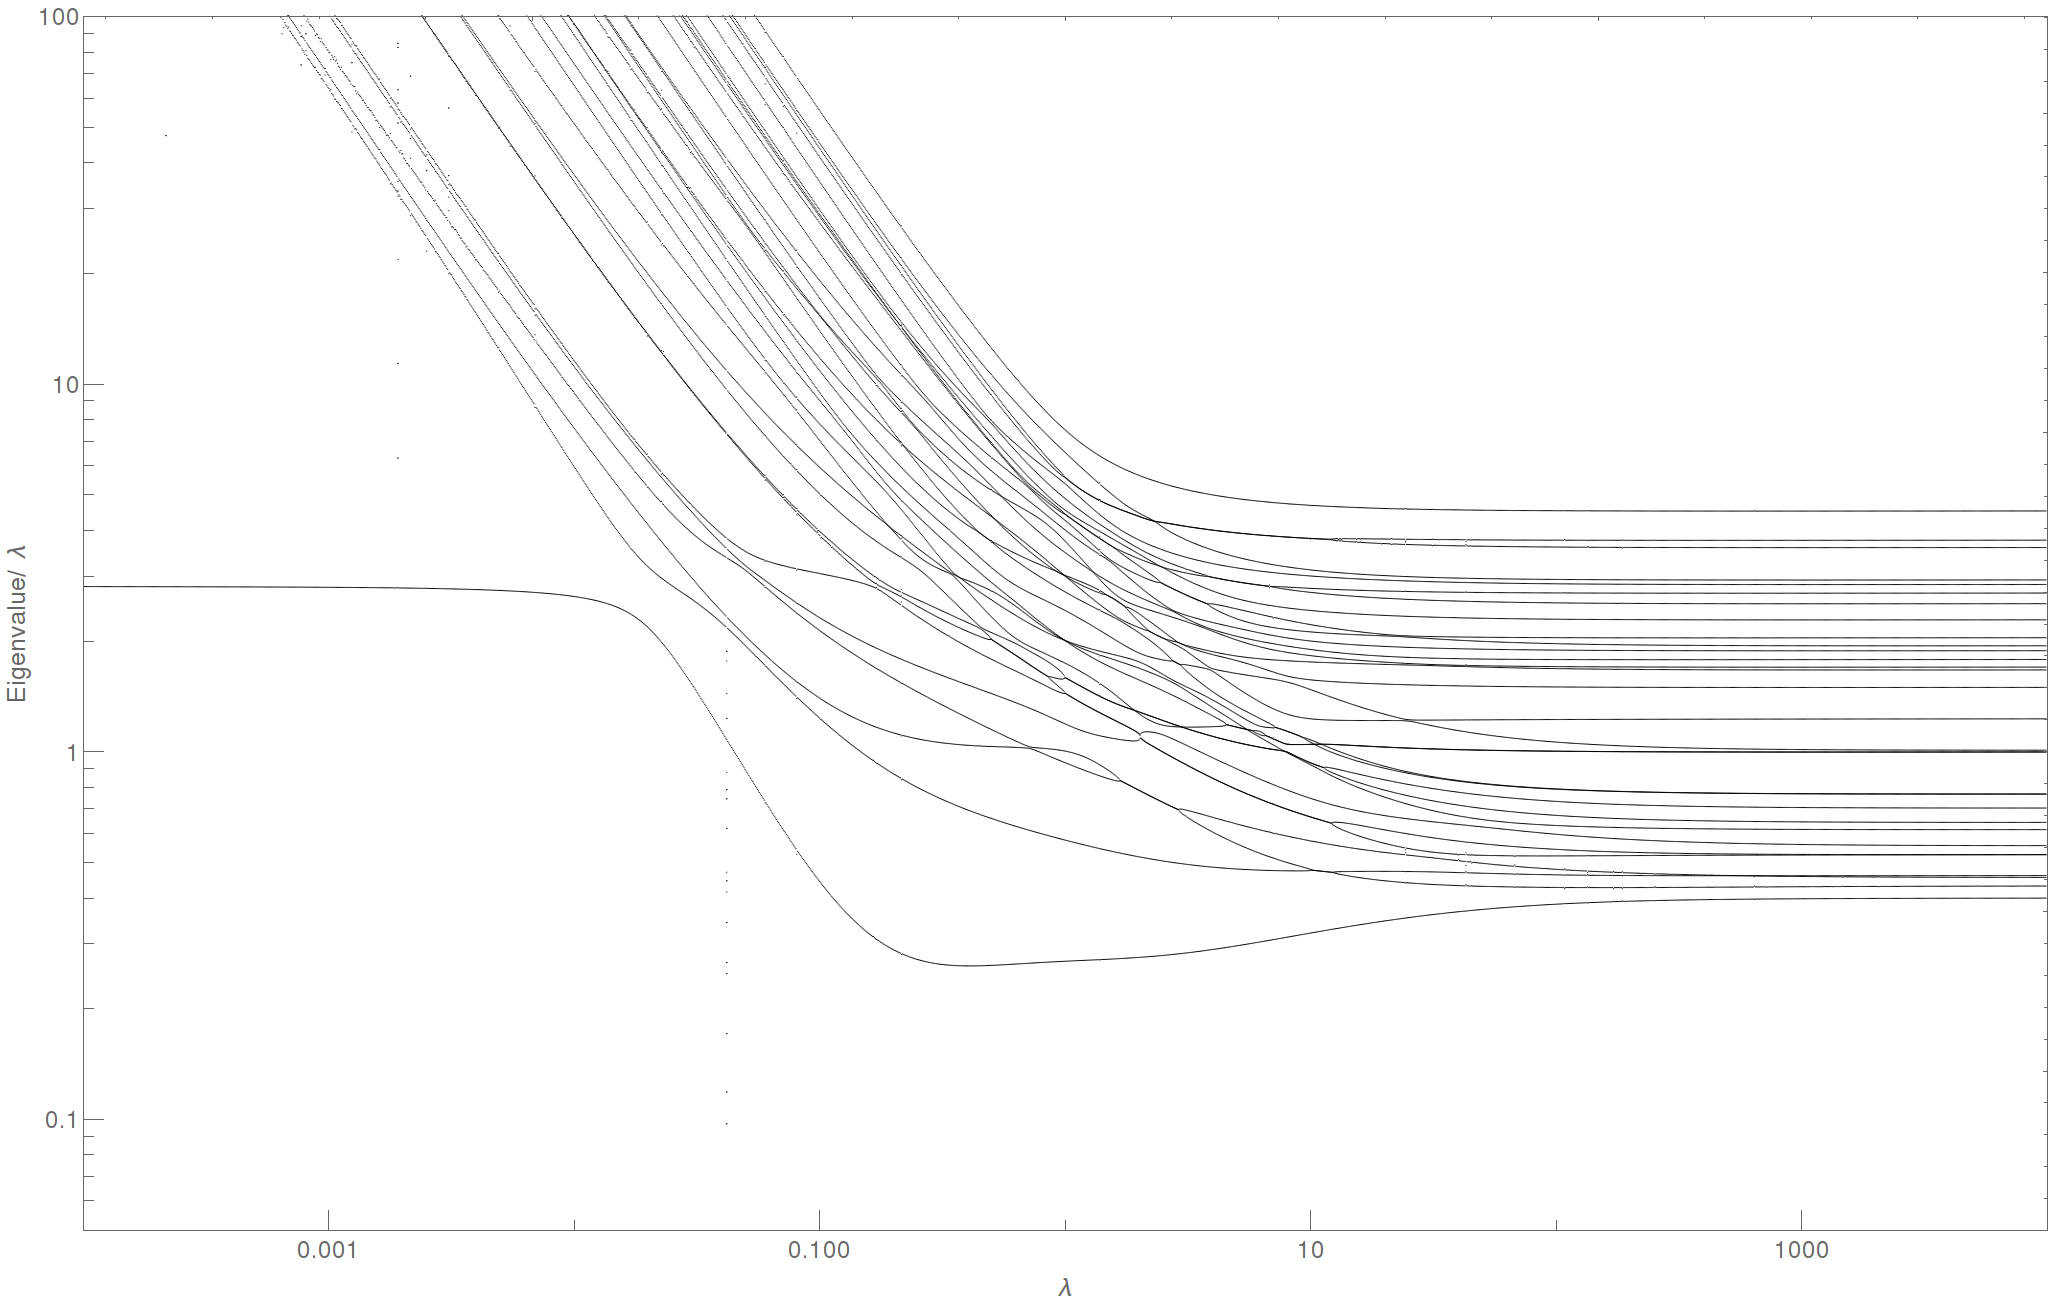
\includegraphics[width=0.9\textheight, angle=270]{TRM/images/singleMultEigB1000L5}
  \end{center}
\end{figure}
\clearpage
}
Of course, for such a system we expect that all eigenvalues have negative real part,
as we discussed in~\ref{sec:TRMGeneralResults}, so we have chosen to plot the
negative real part divided by $\lambda$ as a function of $\lambda$; the zero eigenvalue,
which we expect to exist and is generally found to exist in numerical terms, has been ignored, as its magnitude is simply an artefact of the numerical calculation and
is therefore meaningless except possibly as a check on the numerics. The decision 
to divide by $\lambda$ was taken because the eigenvalue closest to $0$ (which dominates
approach to equilibrium) mostly scales as $\mathcal{O}(\lambda)$, so plotting without division
uses graph space poorly.

There are a several things to note about this spectrum:
\begin{itemize}
 \item It would appear that, for all $\lambda$, there is a single eigenvalue which
 is closest to $0$ and undergoes no definitive crossing as $\lambda$ varies. At both extremes of
 $\lambda$, it clearly scales as $\mathcal{O}(\lambda)$, but is unusually low in an intermediate regime of $\lambda \in (0.03, 10)$, reaching a minimum at $\lambda \sim 0.3$, which could be
 interpreted as an ``avoided crossing'' with the 0-eigenvalue. This is
 important, as the eigenvalue with smallest negative real part is the one that controls
 the approach to equilibrium; thus, we can see that around $0.3$ the system should take unusually long to relax from an arbitrary prepared state to equilibrium.
 \item All eigenvalues tend to scale as $\mathcal{O}(\lambda)$ as $\lambda \rightarrow \infty$.
 \item Eigenvalues other than the bottom one tend to scale as $\mathcal{O}(1)$ at small
 $\lambda$. Thus, whilst the overall approach to equilibrium occurs with rate 
 $\mathcal{O}(\lambda)$, there are still plenty of (probably more localised) processes 
 occurring over much quicker timescales, whilst the whole system is sluggish to 
 equilibrate.
 \item The eigenvalues tend to retain their order at the extremes of $\lambda$, 
 but they frequently cross, merge and separate again in the intermediate regime. This suggests that something complicated is occurring; an analytic solution to this dynamical model would need to describe these crossings in detail, as they are important as
 eigenvalue crossing implies the appearance of degenerate eigenspaces in the decay modes
 which the associated eigenvectors refer to. This makes it look rather 
 unfeasible that such an analytic solution could be constructed in the first place.
\end{itemize}
Of course, this is only the $32$ lowest eigenvalues; there could be different behaviour
in the higher ones. Before we perform a larger calculation however, let us turn our
attention to the dependence of the eigenspectrum upon $b$ and $L$, which we have studied
by repeating our calculation with different values for those parameters, as shown in
Fig~\ref{fig:eigsVarBVarL}.
\afterpage{
 \begin{figure}[h!]
 \caption[The lower part of the TRM eigenspectrum for a system with $L=\{5, 10\}, $, $b=\{100, 1000\}$.]{\label{fig:eigsVarBVarL} 
 The lower TRM eigenspectrum, computed for a system with $\rho_0 = 0.6$, $\rho_L = 0.4$,
 with all combinations of
 $L=\{5, 10\}$, $b=\{100, 1000\}$. Missing computations, visible via the vertical gaps in
 the data, are due to computational issues, rather than being numerically meaningful. Note that
 in many places green/black and blue/red lines overlap, because their results are so similar; the
 image is deliberately prepared in a high resolution so that these intricacies may be observed,
 at least in the digital copy.
 }
  \begin{center}
 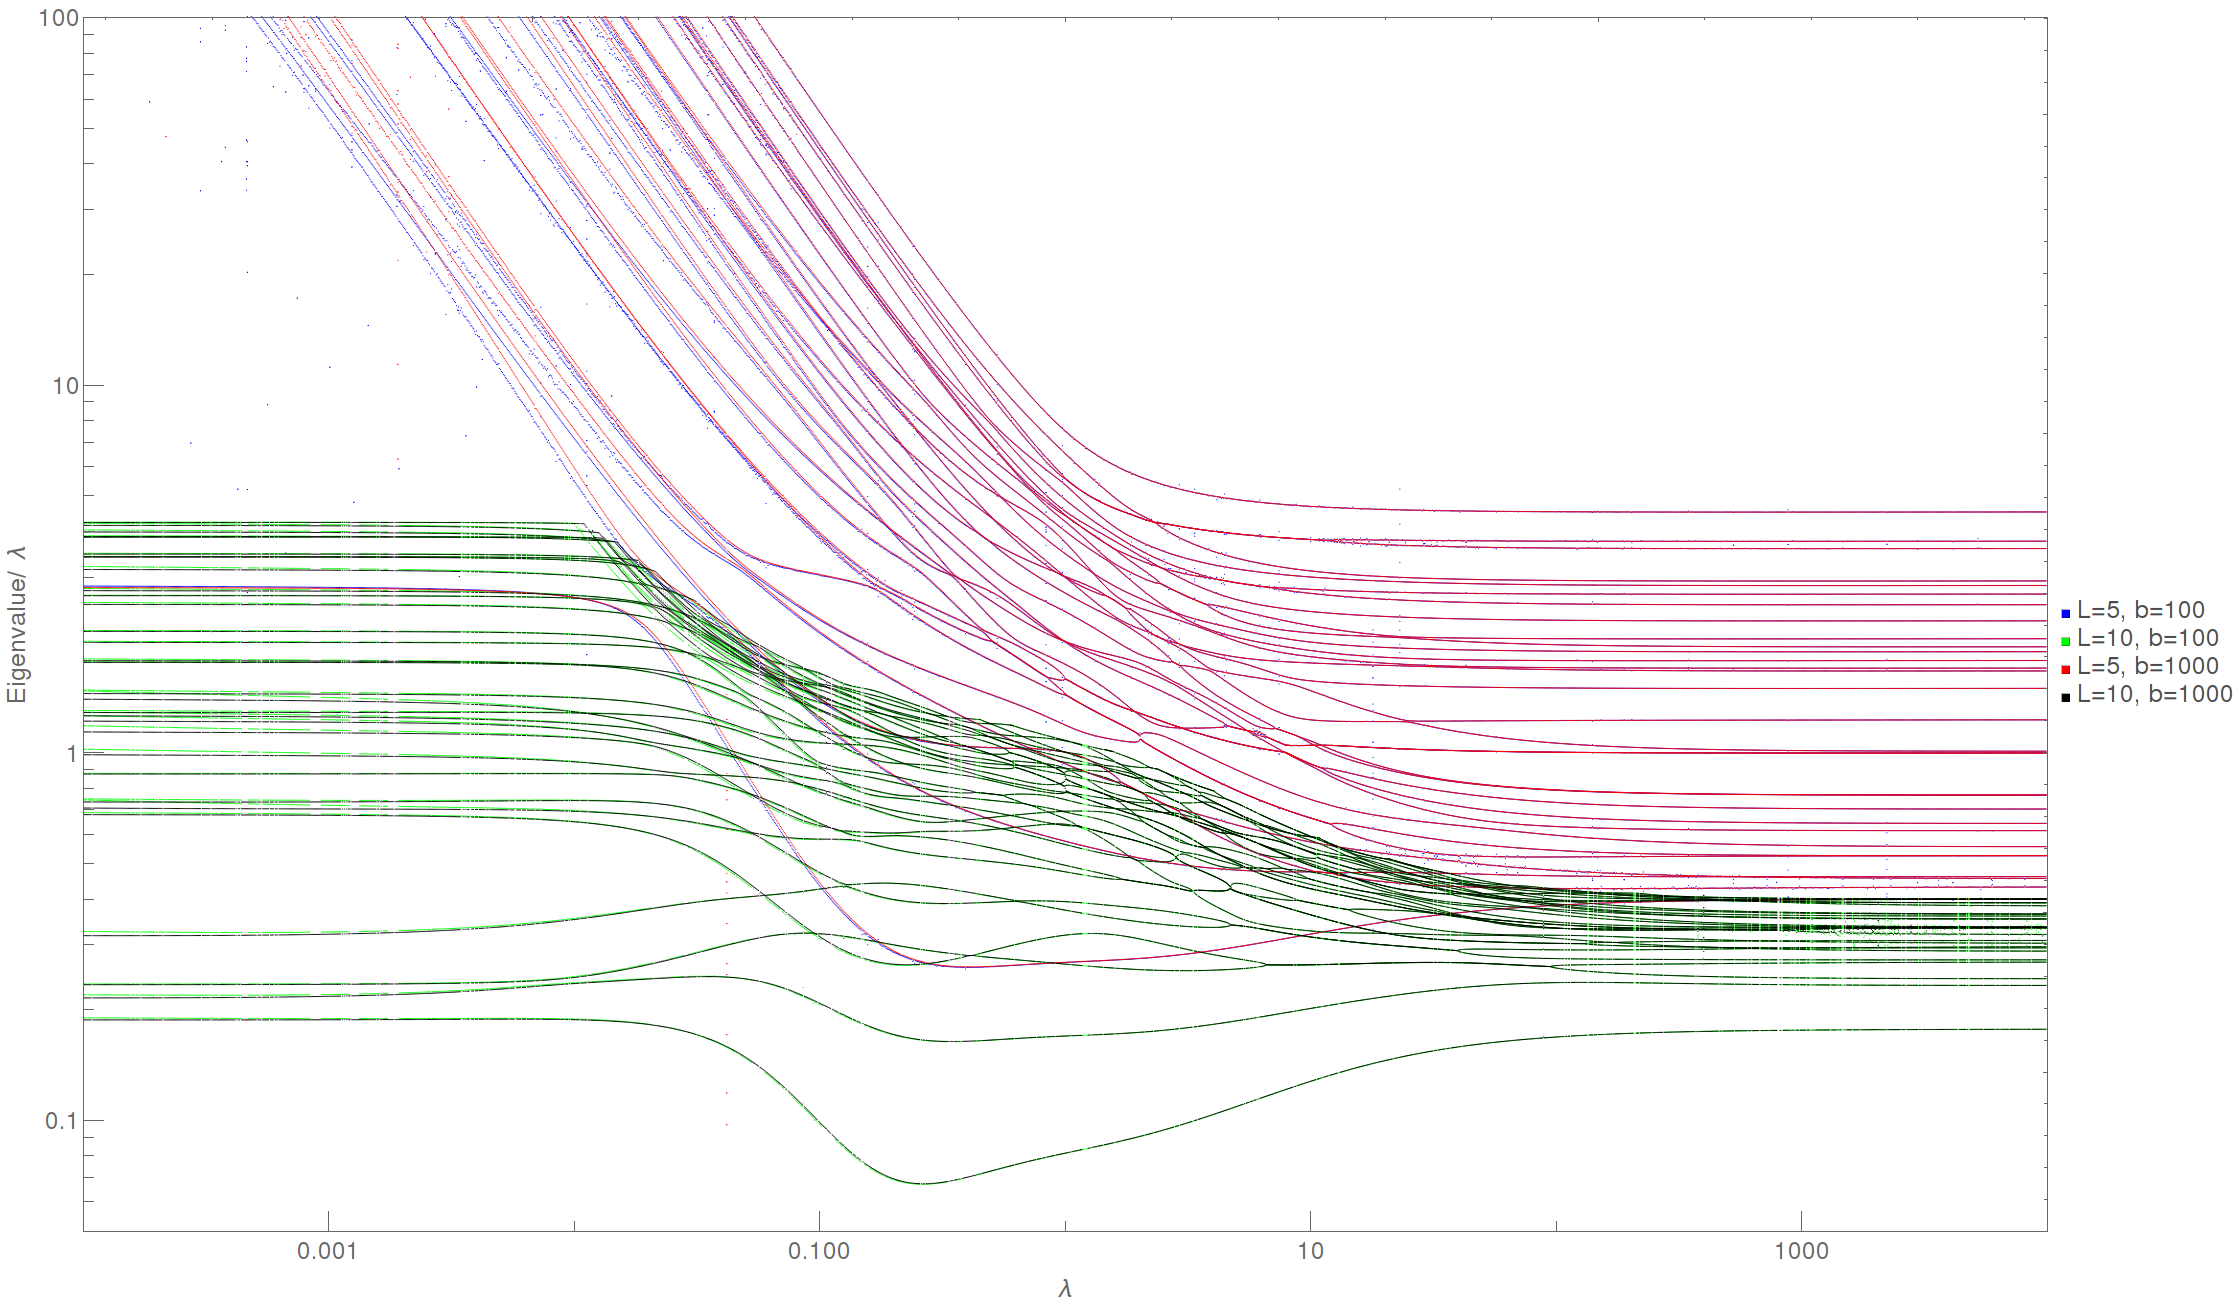
\includegraphics[width=1.0\textheight, angle=270]{TRM/images/repeatRepeatMultEig}
  \end{center}
\end{figure}
\clearpage
}
Again, there's a lot going on in this image, so let's break it down.
\begin{itemize}
 \item Firstly, let us note that keeping $L$ constant and switching $b$ between $100$
 and $1000$ seems to have very little impact on the eigenspectrum, as we can see by the fact that the points corresponding to the same system sizes are
 more or less lying on top of each other unless we delve into the low-$\lambda$ limit
 of the $L=5$ system. In the same limit, we see that the discrepancy is vastly reduced
 in the $L=10$ system, suggesting that it is less bad for large systems, and is in some sense a small-size effect. Regardless, it would appear to be the case that adjusting $b$
 doesn't affect these low-lying eigenvalues very much, so it seems to be playing its
 role as a regularisation parameter as intended. Thus, we're simply going to use $b=1000$
 from now on, unless explicitly specified otherwise.
 \item The bottom eigenvalue, which controls relaxation to equilibrium, is generally
 several orders of magnitude lower for the $L=10$ system than for the $L=5$ one;
 this effect is particularly extreme in the limit of small $\lambda$.
 This makes sense; the larger system should take much longer to equilibrate than the
 smaller one, as so many more fluctuations need to occur to make it change its global
 state. This is something we should remember for later, as it suggests that equilibration time might scale
 pretty aggressively with system size, which is bad news for our attempts to simulate
 the system using Monte-Carlo methods (Ch.~\ref{sec:numerics}).
 \item The big, obvious difference between the spectra of different system size is
 the behaviour at small $\lambda$. For $L=5$ there is only $1$ eigenvalue which scales
 as $\mathcal{O}(\lambda)$ as $\lambda \rightarrow 0$, whereas for $L=10$, it would
 appear that they all do!
\end{itemize}
The last point begs the following question: how does the number of eigenvalues
corresponding to ``slow modes'' at small-$\lambda$ scale with the system size? This is 
important,
because it determines how many of the available decay modes would tend to persist for any 
meaningful amount of time during the relaxation towards equilibrium. We will attempt to
address this in the next subsection.

\subsubsection{The Scaling of the Number of Slow Modes at Low $\lambda$}
To find out how the number of nonzero eigenvalues in the $\mathcal{O}(\lambda)$-scaling
band (as observed in Fig.~\ref{fig:eigsVarBVarL}) scales with system size,
we can simply fix $\lambda$ to be sufficiently low (say, $\lambda=0.0001$)and repeat
computations of the low-lying eigenspectrum for different $L$. Here, due to the
computational limitations we are up against, we only compute up to $L=13$. The number
of slow modes as a function of $L$ is displayed in Tab.~\ref{tab:bandThickness}.
\begin{table} \caption[Tabulated values for the variation of the width of the slow band with
system size.]{A table of the number of slow modes occurring at low $\lambda$ for given 
$L$.}
\begin{center}
\begin{tabular}{r || r | r | r | r | r | r | r | r | r | r | r | r} \label{tab:bandThickness}
 $L$ & 5 & 6 & 7 & 8 & 9 & 10 & 11 & 12 & 13 \\
 \hline
 Bandwidth & 1 & 3 & 6 & 11 & 20 & 36 & 64 & 113 & 199 \\
\end{tabular}
\end{center}
\end{table}
If we plot the number of slow modes as a function of system size on a plot with a 
logarithmic $y$-axis, as we have done in Fig.~\ref{fig:bandWidthScaling},
it is rather obvious that the bandwidth scales exponentially with system size.
However, the number of slow modes seems to scale as $\mathcal{O}(2^{\sim 0.84 L})$,
whereas the number of possible states, and therefore the total number of eigenvalues of
the TRM, scales as $2^L$. Thus, one can see that although the number of slow modes grows
very aggressively with the system size, it would appear to eventually become 
outpaced by the growth in the total number of eigenvalues; in this way, we can say that
the slow band carries increasingly less of the total eigenvalue density as system size
becomes large.
 \begin{figure}[h!]
 \caption[A graph of the scaling of the number of slow modes with system size.]{\label{fig:bandWidthScaling} 
 A plot of the scaling of the number of slow modes in the eigenspectrum of the TRM of
 an SPM system of size $L$. The trendline displayed has equation
 $ \mathrm{Bandwidth} = 2^{a(L+b)}$, with $a=0.84$, $b=-3.9$.
 }
  \begin{center}
 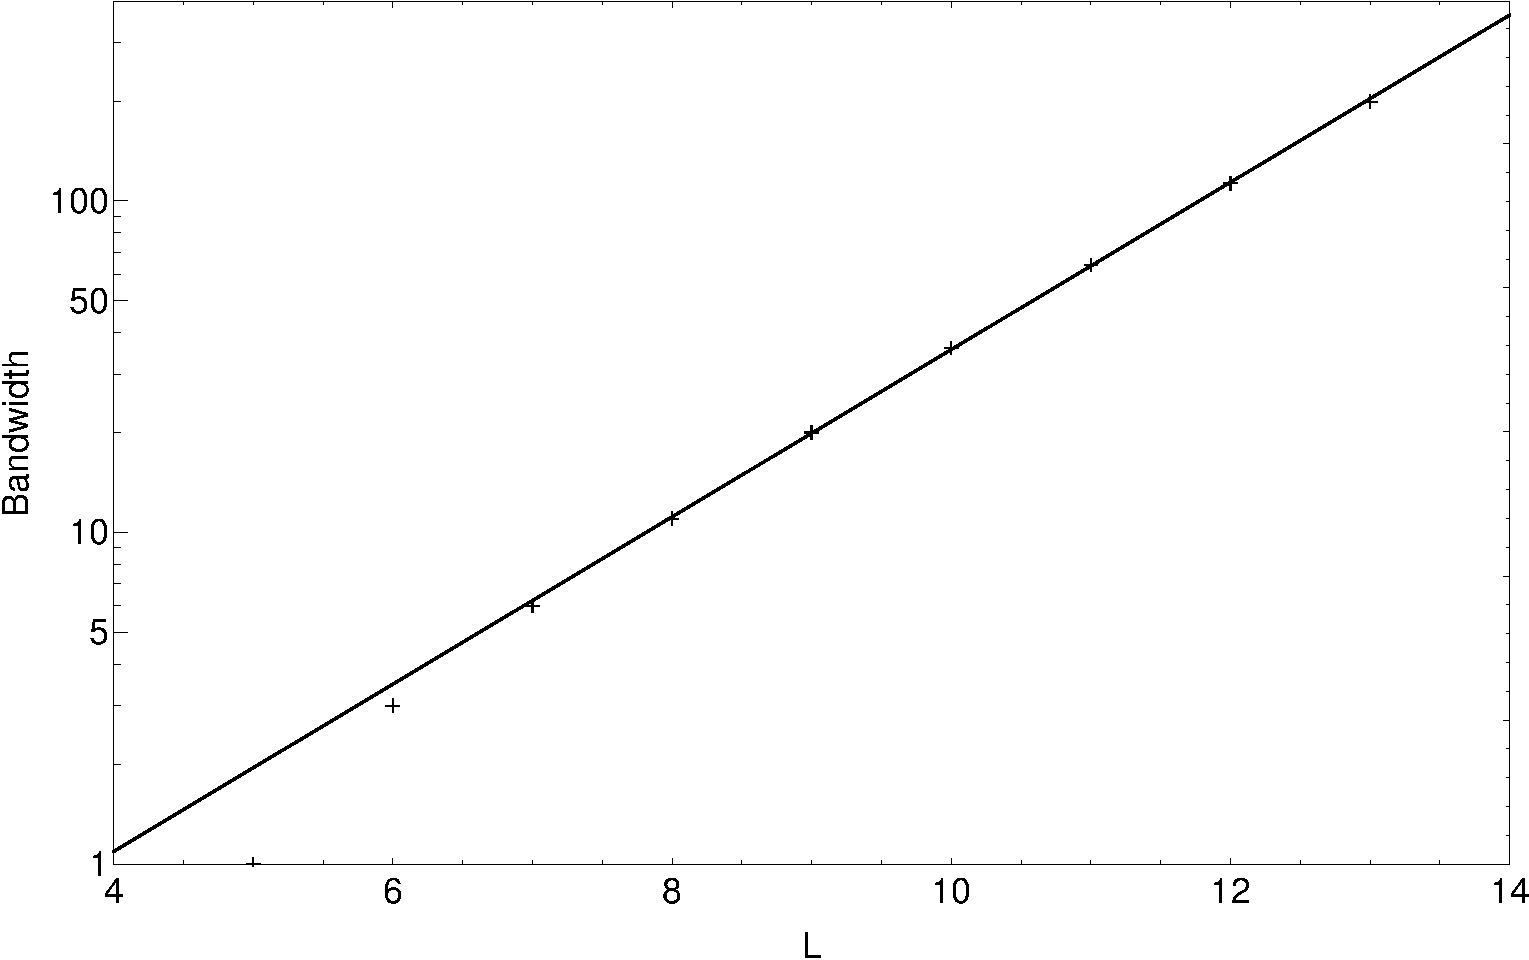
\includegraphics[width=1.0\textwidth]{TRM/images/bandWidth}
  \end{center}
\end{figure}

\subsubsection{The Upper Part of the Spectrum}

By varying $L$ and $b$ and analysing the lower (more physically relevant) part of the
TRM eigenspectrum, we concluded that $b$ has very little impact and essentially
acts as a regularisation parameter, whilst $L$, the system size, has a large impact,
particularly on the approach to equilibrium. However, both $b$ and $L$ contribute to
the actual numbers contained within the TRM, so it stands to reason that they must
impact the eigenspectrum in some way. Therefore, we have done an additional check,
by varying $b$ and $L$ and 
performing a calculation in which the $64$ eigenvalues with largest negative real
part were calculated. The negative real parts of these eigenvalues are displayed in
Fig.~\ref{fig:eigsVarBVarLUpper}.
 \begin{figure}[h!]
 \caption[The upper TRM eigenspectrum for a system with $L=\{5, 10\}, $, $b=\{100, 1000\}$.]{\label{fig:eigsVarBVarLUpper} 
 The upper TRM eigenspectrum, computed for a system with $\rho_0 = 0.6$, $\rho_L = 0.4$,
 with all combinations of
 $L=\{5, 10\}$, $b=\{100, 1000\}$.
 }
  \begin{center}
 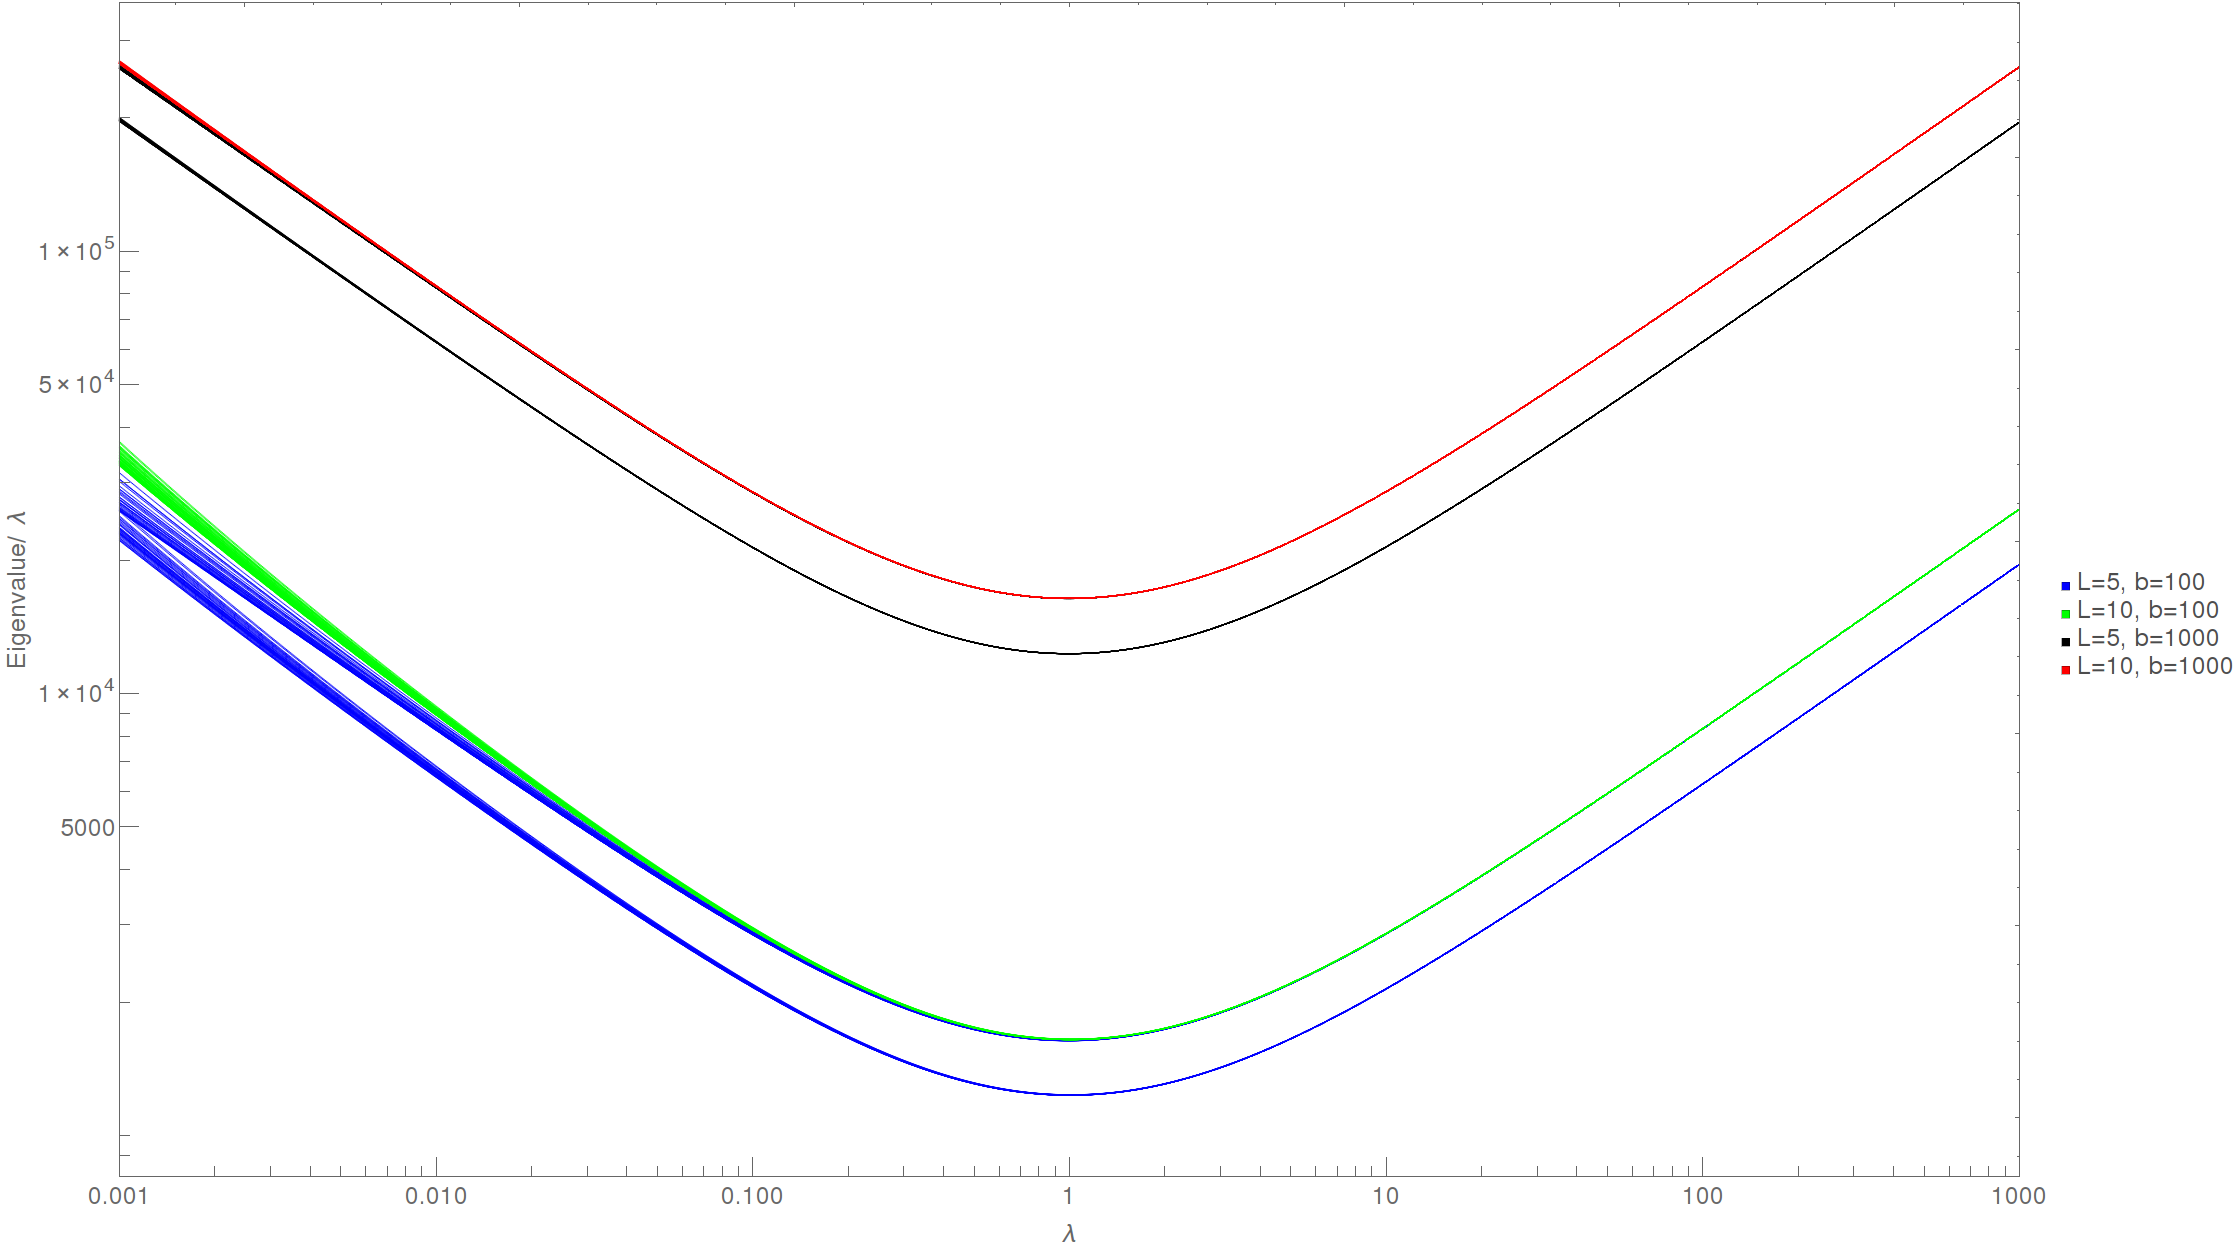
\includegraphics[width=1.0\textheight, angle=270]{TRM/images/topEigs}
  \end{center}
\end{figure}
We see that now the tables are indeed turned. Altering $L$ does have a very small effect on
the upper band, as we can see by how the red/black and blue/green points lie on top
of each other. On this graph, we see that for the $L=5$ datasets there are apparently
two bands, whilst for $L=10$ there is only one; however, recall that we have produced
this by plotting the negative real parts of the $64$ eigenvalues with largest negative
real part; thus, as the $L=10$ systems have $2^5 = 32$ times as many eigenvalues in 
total, it makes sense that we may not have finished the very top band in the $L=10$
case yet whilst we have moved on to the second band in the $L=5$ case; thus, we conclude that
system size has little effect on the top of the eigenspectrum.

The value of $b$, however, has a huge impact, as it determines the overall magnitude
of these larger eigenvalues. The eigenmodes associated with them almost certainly
relate to fluctuations at the boundary, and then the ensuing joint fluctuations 
travelling a little into the bulk. As these are boundary effects, it again makes sense
that $L$ has little impact. The value of $b$ directly controls the speed of the 
fluctuations at the boundary, thus the large shift in magnitude observed should be 
expected.

\subsubsection{Large Calculation}
Now that we are more or less satisfied that the value of $b$ doesn't matter so long as
it's quite large, let's perform a similar calculation (sweeping through $\lambda$ with
constant boundary conditions), but this time compute a lot of eigenvalues in order to
get a general overview of the TRM. 
\afterpage{
 \begin{figure}[h!]
 \caption[The ``full'' TRM eigenspectrum for a system with $L=8, $, $b=1000$.]{\label{fig:bigEigSpec} 
 The ``full'' TRM eigenspectrum, computed for a system with $\rho_0 = 0.6$, $\rho_L = 0.4$,
 with $L=8$, $b=1000$. Missing computations, visible via the vertical gaps in
 the data, are due to computational issues, rather than being numerically meaningful.
 }
  \begin{center}
 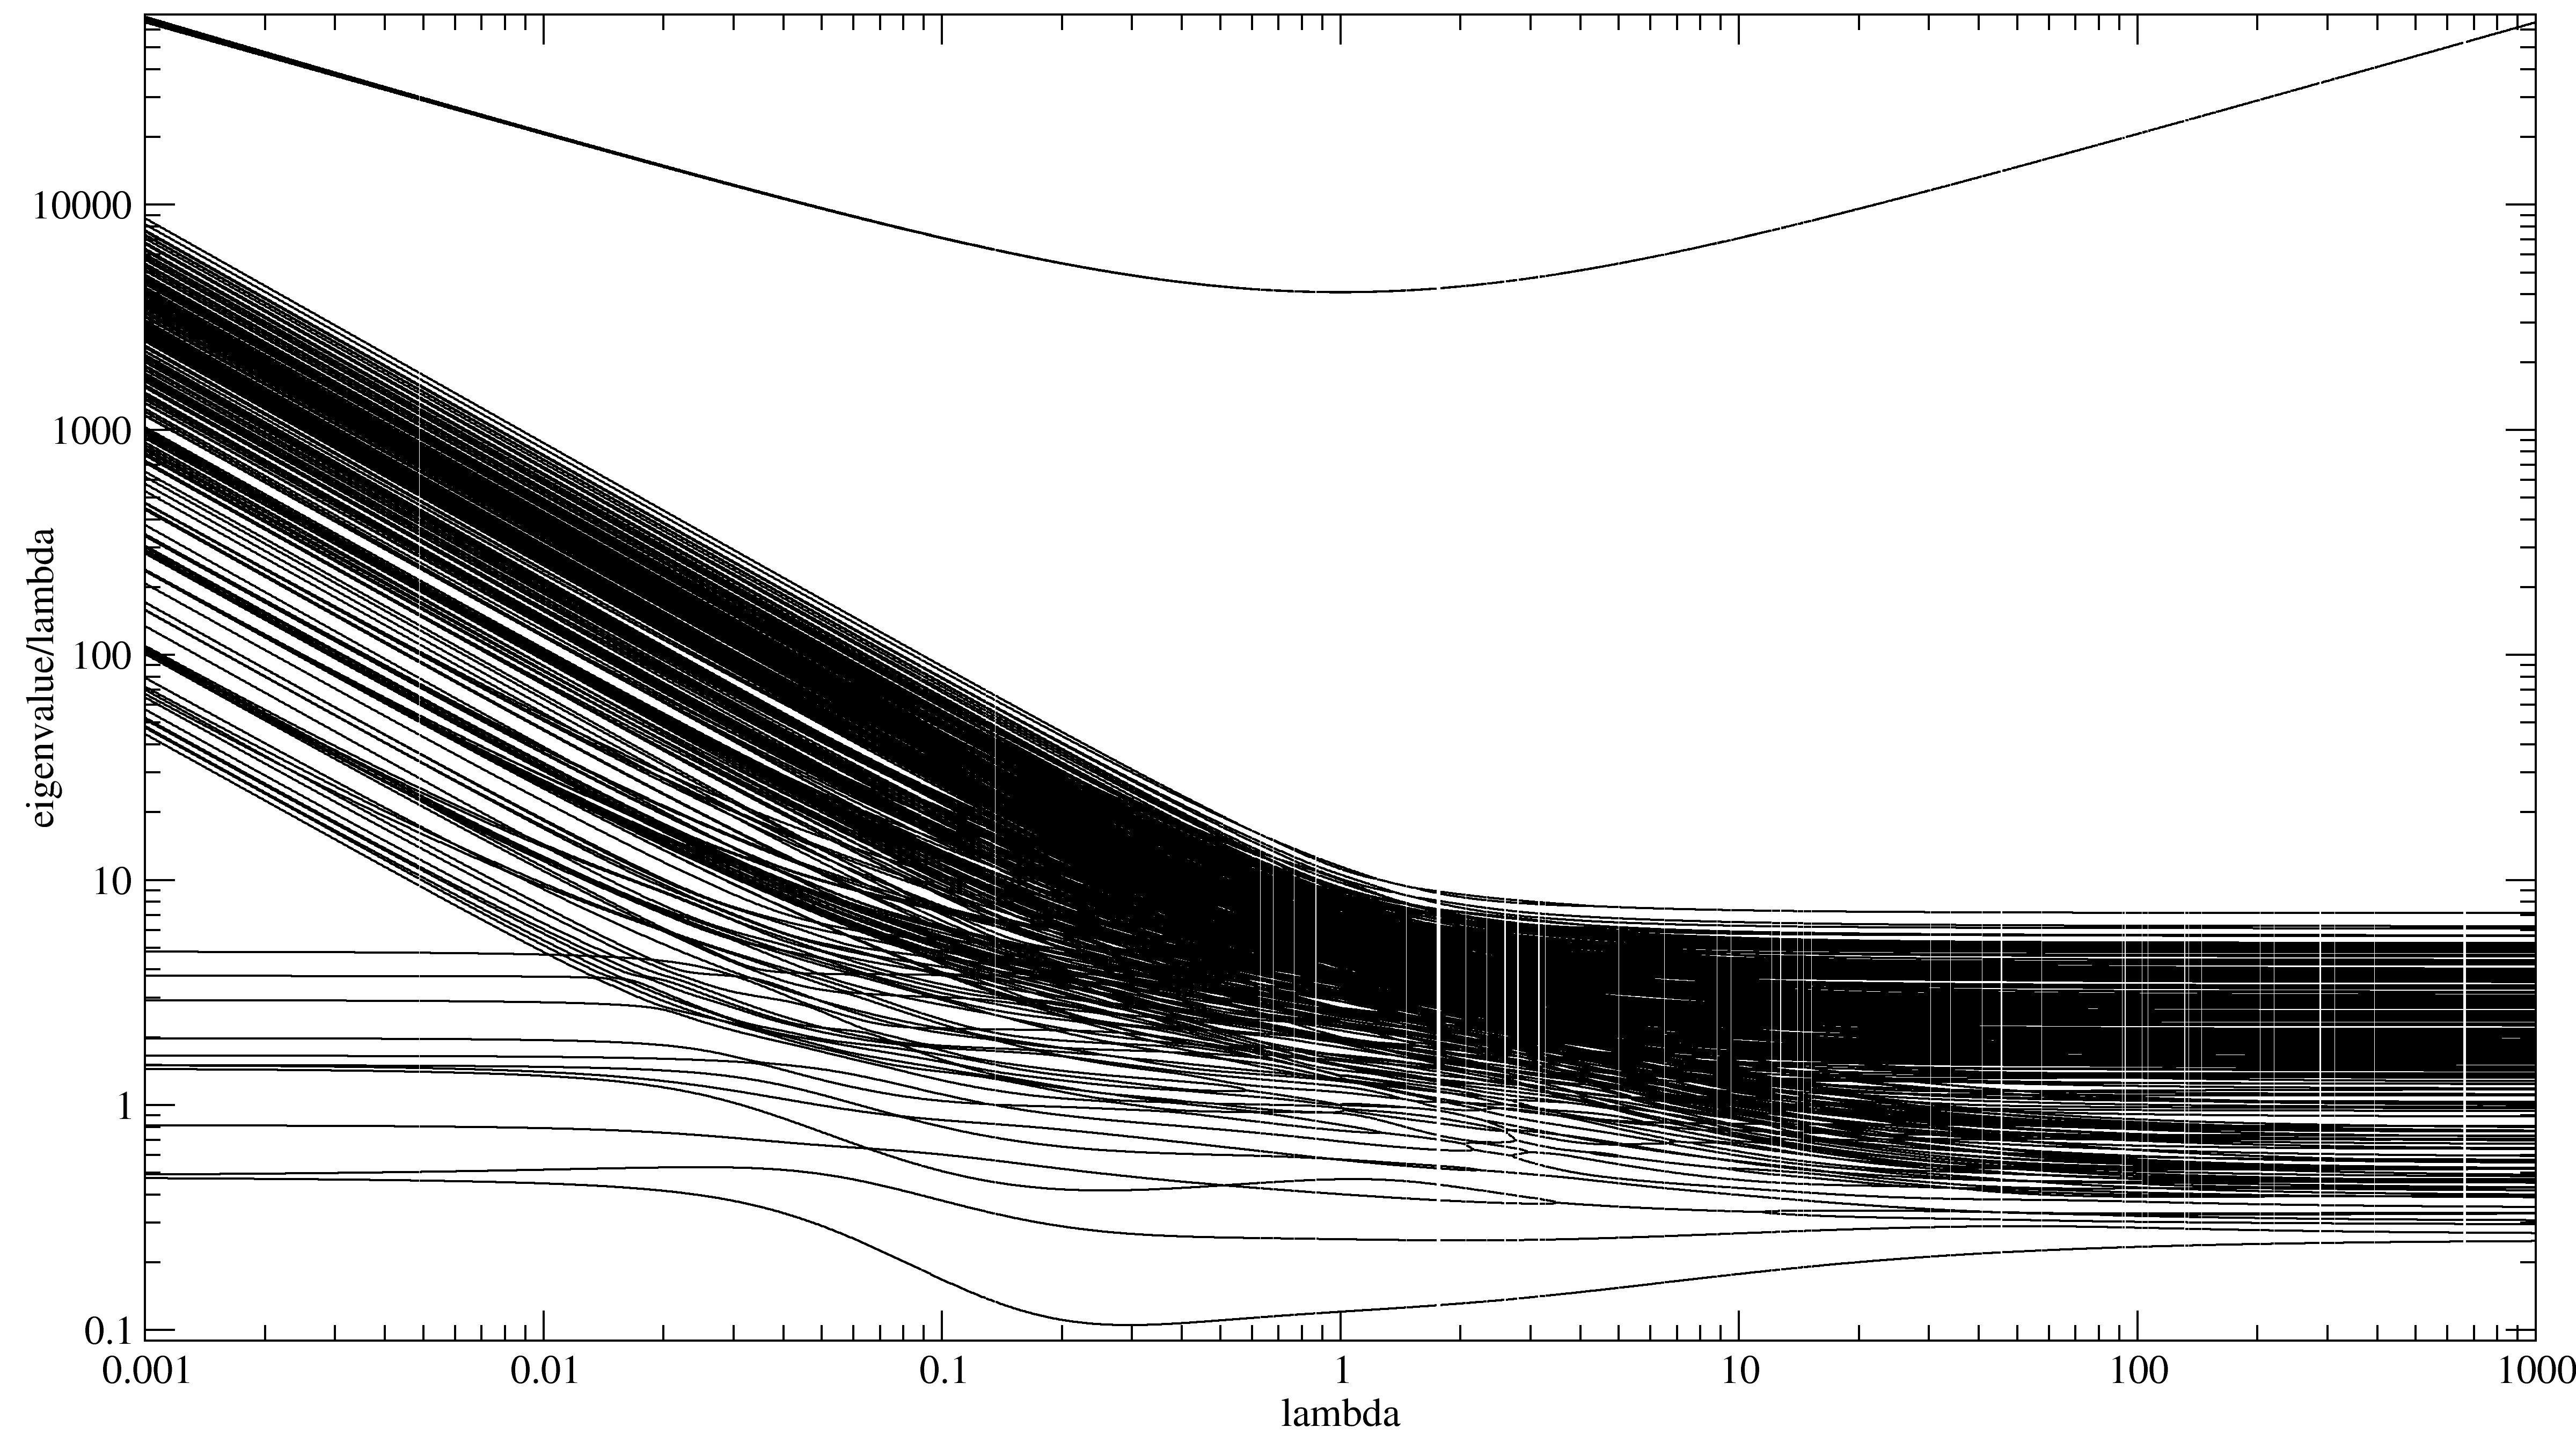
\includegraphics[width=0.9\textheight, angle=270]{TRM/images/bigEigSpec}
  \end{center}
\end{figure}
\clearpage
}
Plotted in Fig.~\ref{fig:bigEigSpec} are the negative real components of the $1024$ eigenvalues with smallest negative
 real part, for the TRM of an SPM system of length $L=8$ and regularisation parameter 
 $b=1000$. We say that this is the ``full'' eigenspectrum not because
 we have computed all of the eigenvalues (we have not, as there are $2^{12} = 4096$ in
 total), but because the eigenvalues with very large negative real part seem to converge
 upon each other, forming the hyperbola-shaped entity towards the top of the graph.
 We believe that this is because the relevant dynamical modes correspond to extremely rapid changes in system state which are limited to the region immediately around the boundaries; as these should
 have no impact on large-scale properties such as the current, they are of very limited
 interest
 to us.
 
This large computation continues the themes we have seen in the small ones:
\begin{itemize}
 \item For large $\lambda$ there is a thick band of eigenvalues spread over a couple
 of orders of magnitude which scale as $\mathcal{O}(\lambda)$.
 \item For intermediate $\lambda$ the bottom eigenvalue becomes unusually small, whilst
 the higher ones in the thick band are constantly crossing over each other.
 \item As we go to small $\lambda$ a thin band of $\mathcal{O}(\lambda)$-scaling
 eigenvalues split off from the main sequence, which scales as $\mathcal{O}(1)$.
 \item For all $\lambda$ there is the hyperbola-shaped band of eigenvalues with highly
 negative real part, which are many orders of magnitude different to the main sequence;
 thus, their dynamics operate over an extremely short timescale, and they are almost
 certainly attributable to the flickering motion at the boundaries.
\end{itemize}



\subsection{Current and Density in the Steady State} \label{sec:TRMDensityCurrent}
The eigenvectors of the TRM correspond to decay modes, and in general contain both 
positive and negative components; thus, they do not in general correspond to a
particular distribution, only to a time-dependent part of a sum of vectors on their
way to equilibrium. The exception to this is the $0$-eigenvalue eigenvector, which
\textbf{does} correspond to a physical state, if properly normalised.

Given a vector corresponding to a normalised probability distribution, we can extract
the mean occupation of its $i^\mathrm{th}$ site by taking the inner product of the
distribution vector with a vector which has component $1$ on states in which the
$i^\mathrm{th}$ sites is occupied and $0$ otherwise. Thus, we can construct an operator
$\mathrm{P} : \Xi \rightarrow \mathbb{R}^{L+4}$ which can tell us the density profile of
the system given its ground state, which we have found using the linear algebraic
methods discussed in Sec~\ref{sec:eigenFind}. We can create a similar operator
$J : \Xi \rightarrow \mathbb{R}^{L+3}$ which gives the current; however, if used on a 
steady state, it simply gives a constant result internal to the system, due to the
existing constraint that particle number is conserved. We can of course extract
the homogeneous current through the system by using this operator and then simply
keeping one of the current components.

\subsubsection{TRM-Computed Density Profile}
By way of example, we computed the density profile for a system with $L=10$, $b=1000$,
again sweeping through a wide range of scales of $\lambda$ as in the previous section.
We kept the boundaries constant with our usual $\rho_0 = 0.6$, $\rho_L = 0.4$
configuration. A density plot of the data is shown in Fig.~\ref{fig:analDensProf}.
 \begin{figure}[h!]
 \caption[The variation of the density profile with $\lambda$ for a system of size
 $L=12$ and boundaries $(\rho_0 = 0.6, \rho_L = 0.4)$.]{\label{fig:analDensProf} 
A coloured plot showing the variation of the density profile with $\lambda$ in steady state for a 
system with boundary conditions $(\rho_0 = 0.6, \rho_L = 0.4)$ of size $L=10$. Note 
that the indices of the internal sites are $3$-$12$ inclusive, as $1$-$2$ and 
$13$-$14$ are reserved for the boundaries, whose densities are already prescribed and therefore aren't plotted here.
 }
  
  \begin{center}
 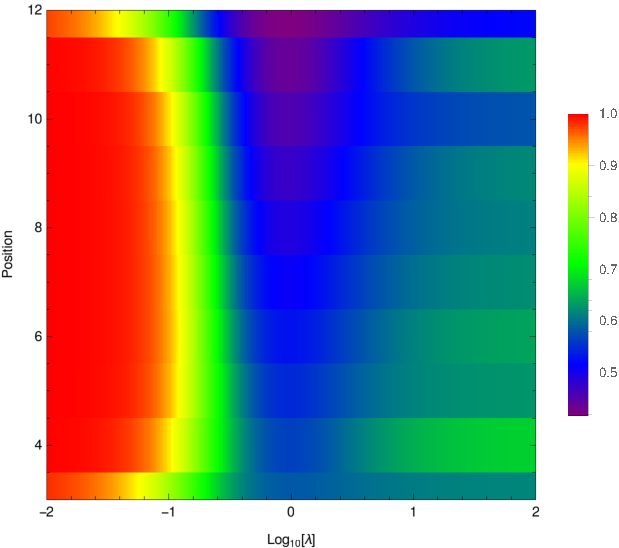
\includegraphics[width=1.0\textwidth]{TRM/images/analMidDensProfile}
  \end{center}
\end{figure}
 Looking at $\lambda=1$, we see that there is a roughly constant gradient for the density profile between the
 boundaries, which makes sense as this is the simple exclusion limit, so it's essentially just normal
 diffusion.
 As we go to smaller $\lambda$, we see that the system in general is quite full. Presumably this is because
 material has been sucked into the system due to the attraction implied by the small $\lambda$; this
 indicates that the boundaries used are a bit odd in this limit, as the system might not naturally form
 a homogeneous phase for such a $\lambda$ and could instead wish to form a mixture of lower and 
 higher density clumps. 
 
 Our theory about why this occurs is as follows.
 At large 
 $\lambda$, we see that the density profile defaults to $\rho\sim\frac{2}{3}$ plus oscillations on the 
 boundaries which decay as we go towards the interior. This is suspiciously close to the critical density
 of the MFT (Ch.~\ref{sec:analChap}) which permits a maximal flow; therefore, we suggest that the system
 self-organises at high $\lambda$ to favour configurations that permit high current. The reason this density permits a high current is that in such a configuration,
 any particular particle should on average be in contact with an adjacent particle, with a free space to move into, so the dynamics of the system should be dominated by $\lambda$ rather than $1$. If the density were
 higher, some particles don't have spaces to move into, so that will slow things down; if the density were 
 lower, particles aren't receiving the speed benefit of being a neighbour. We believe that this 
 self-organisation occurs in the bulk, with thin boundary layers occurring near to boundaries
 with densities fixed away from $\frac{2}{3}$ .
 We believe that this thin layer is revealed by the oscillatory layer observed near to the boundaries; right next to the boundary, in alternating sites, particles will tend to
 linger in sites where they are alone, rapidly leaving when they are prompted by the arrival of a new particle in 
 the  space next to them. This effect then smooths out as one goes deeper into the bulk.
 
 As for why a density which permitted fast flow would be favoured, consider what happens when a 
 region of low flow comes into contact with one of high flow: the high-flow region will invade the
 other region with particles or vacancies, raising the overall flow rate (which previously would
 have been limited by the slowest-flowing region) and thus flushing out or bringing in new 
 particles. In this way, the system as a whole will tend to favour the fast-flow densities, as
 they are more stable than the alternatives. We discuss more numerical data about the system density
 in Sec.~\ref{sec:lambdaScans}, and that seems to generally support the conclusions we have reached
 here using our TRM method.
 
 \subsubsection{TRM-Computed Current} \label{sec:TRMLambdaScan}

 Whilst we computed the density profile, we also measured the steady state current. We also performed the
 same computation for different boundary conditions, and the results are displayed in Fig.\ref{fig:analCurr},
 along with the corresponding MFT prediction. Note that some of these calculations failed, hence 
 the gaps in the spectra.
\afterpage{
 \begin{figure}[h!]
 \caption[The variation of the current (measured flowing from high density boundary to
 low) with $\lambda$ for a system of size
 $L=10$ and boundaries $(\rho_0 = 0.6, \rho_L = 0.4)$.]{\label{fig:analCurr} 
A logarithmic plot showing the variation of current with $\lambda$ in steady state for a system with boundary conditions $(\rho_0 , \rho_L )$ as indicated with system size $L=10$. 
The current measurement is oriented so that positive current corresponds to flow
from high density to low (the normal case). The relevant MFT prediction is shown via a dashed line in each
case.
 }
  \begin{center}
 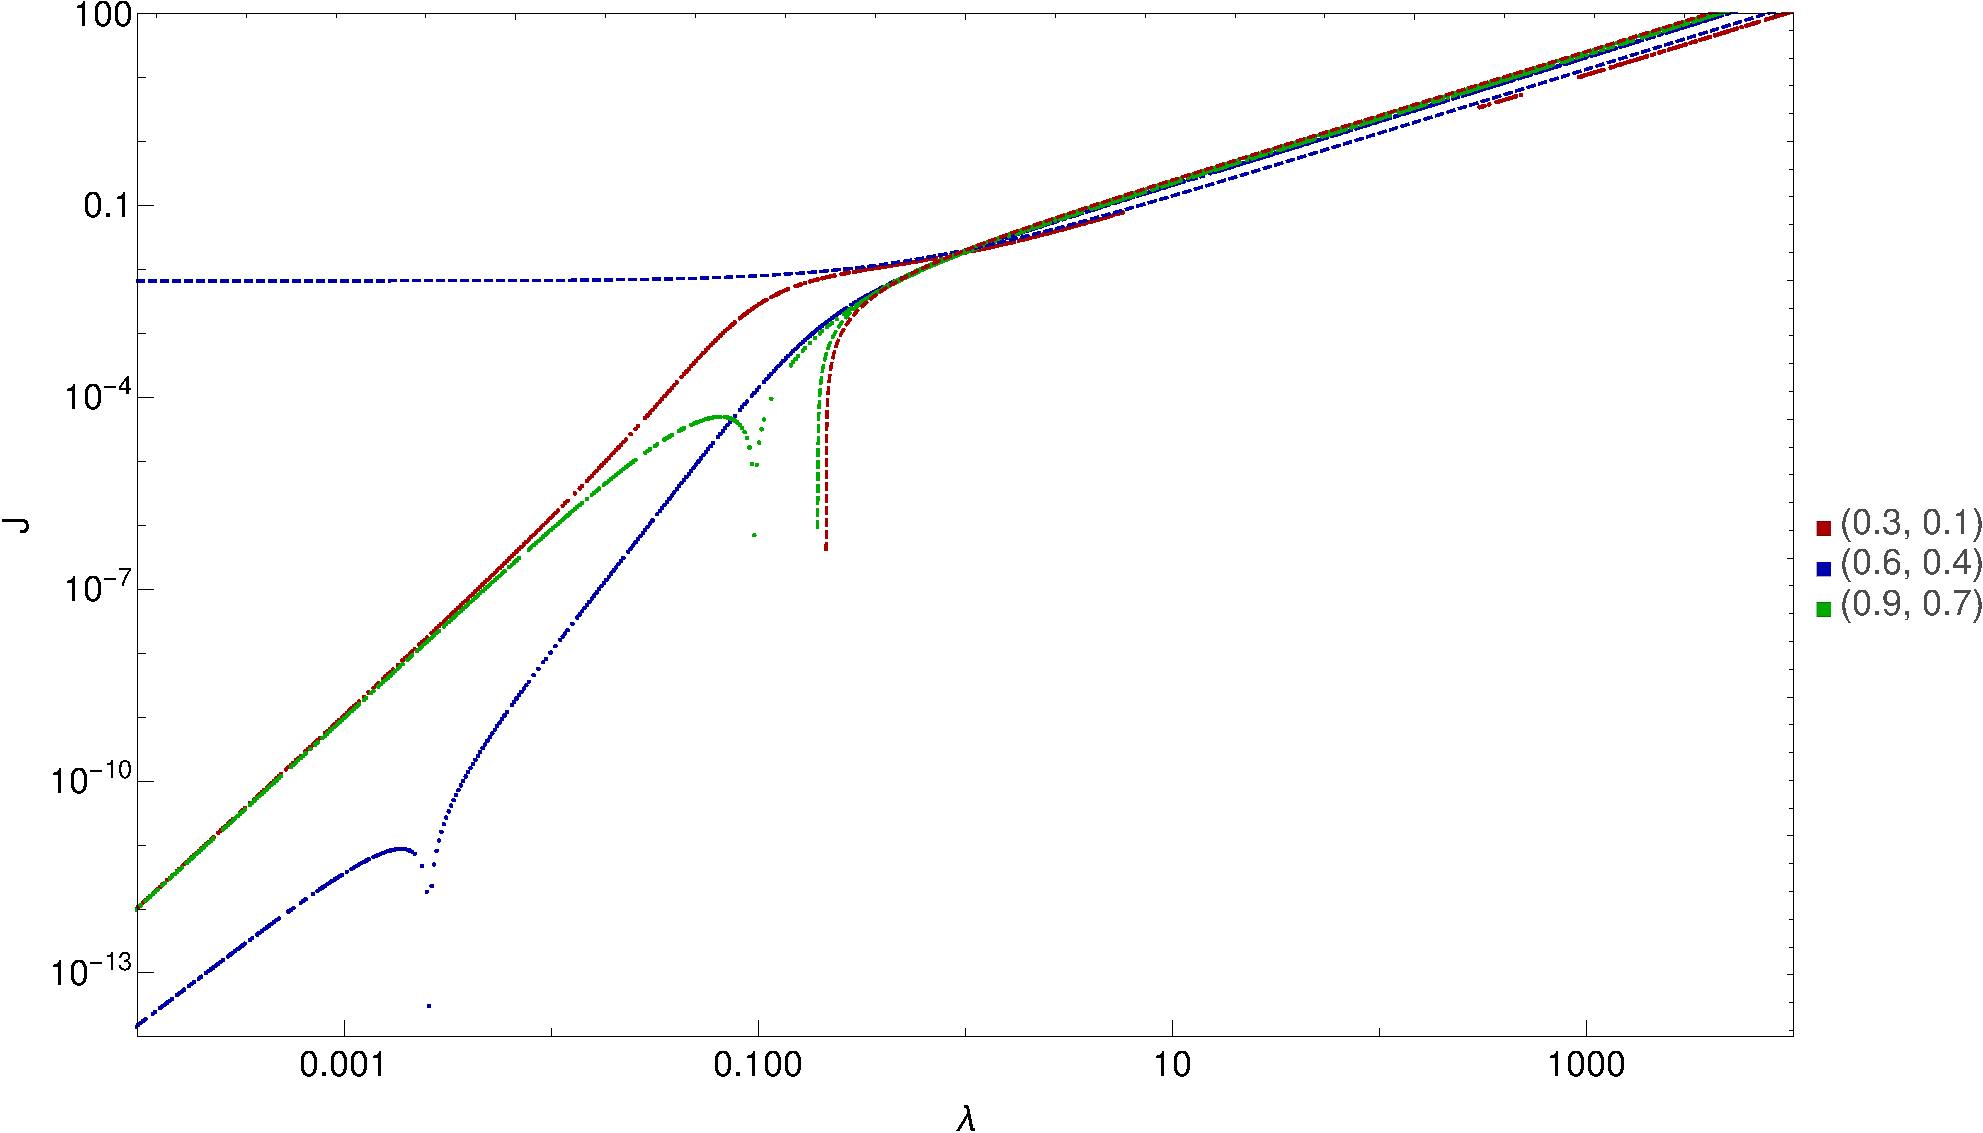
\includegraphics[width=0.9\textheight, angle=270]{TRM/images/TRMMFTCurrCombPlot}
  \end{center}
\end{figure}
\clearpage
}
There's a lot going on here, so let's break it down.
\begin{itemize}
 \item At large $\lambda$, we see that the scaling ($\mathcal{O}(\lambda)$) is the same for both the MFT
 and the TRM numerics. The actual values predicted by the MFT and the TRM calculations differ slightly,
 but not by a great deal until we have $\lambda < 1$. It is to be expected that there is a discrepancy,
 as the MFT is in the continuum-limit whereas the TRM system is only of size $L=10$. Furthermore, there
 should be a discrepancy anyway as the TRM system is not mean-field; it just doesn't seem to be so relevant
 in this regime.
 \item At $\lambda=1$, MFT and TRM calculations coincide, because the boundary conditions all differ
 by the same amount and $\lambda=1$ is the trivial case of simple exclusion.
 \item As we explore very small values of $\lambda$, we find that the MFT and the TRM have very little 
 resemblance. For boundary conditions $(0.3, 0.1)$ and $(0.9, 0.7)$ the MFT predicts that the flow should
 start running backwards or at the very least be pinned at zero,
 whilst for $(0.6, 0.4)$ it suggests that the current should tend to a constant
 as $\lambda \rightarrow 0$. 
 Instead of the flow crashing to zero, the TRM results show a more gradual reduction of the current.
 Measurement by comparison with a trendline shows that the current varies as $\mathcal{O}(\lambda^3)$ as 
 $\lambda$ becomes small.
 \item There is an intermediate regime in which the dependence of the current upon $\lambda$ transitions
 between $\mathcal{O}(\lambda^3)$ and $\mathcal{O}(\lambda)$. This is the situation for $\lambda \in (0.03, 0.5)$.
 \iffalse
 \item There is also some slightly odd behaviour on display in terms of the apparent ``poles'' in the 
 current for
the $(0.6, 0.4)$ and $(0.9, 0.7)$-boundaried systems. This could be due to a close-approach of eigenvalues,
causing the algorithm to pick the wrong one under certain circumstances. We have filtered the results by
imposing the inequality $\| q_0 \| \le \lambda K$ for $K=10^{-9}$ with $q_0$ being the ``zero'' eigenvalue,
but some results may have slipped through this net. We think this is the most likely explanation we have to
hand.
\fi
\end{itemize}
So, it seems that whilst we don't see a transition to zero flow as predicted by the MFT, we do see
a big change in the way the flow depends upon $\lambda$ as we pass between the large-$\lambda$ to 
small-$\lambda$ regimes.


\subsubsection{TRM-Computed Diffusion Coefficient}
It is also possible for us to compute an approximation to the effective diffusion coefficient.
Recall that the diffusion coefficient $D$ should satisfy
\begin{equation}
 \mathbf{J} = -D \mathbf{\nabla} \rho ;
\end{equation}
thus, we should be able to compute the diffusion coefficient using the TRM by computing the current $J$
with boundary conditions $(\rho_0, \rho_L) = (\rho+\frac{1}{2}\delta\rho, \rho-\frac{1}{2}\delta\rho)$,
and then evaluating the quantity
\begin{equation}
 D(\rho, \lambda) = \frac{L}{\delta \rho} J.
\end{equation}
We performed such a calculation, in which we picked $\delta \rho$ to be $0.001$ and $L=10$. We tabulated
$D$ for a range of $\lambda$ and $\rho$, and a contour plot of the data is displayed in 
Fig.~\ref{fig:TRMDiffCoeff}.
 \begin{figure}[h!]
 \caption[The variation of the diffusion coefficient of a system of size $L=10$ with respect to $\lambda$
 and $\rho$.]{\label{fig:TRMDiffCoeff} 
A coloured plot showing the variation of the diffusion coefficient with $\lambda$ and $\rho$
in steady state for a 
system of size $L=10$.
 }
  \begin{center}
 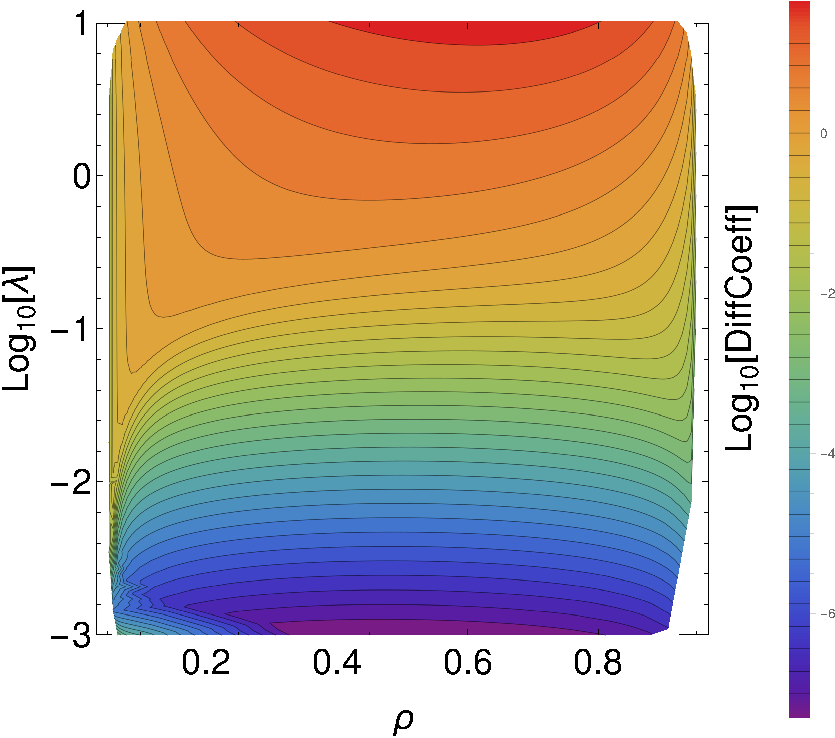
\includegraphics[width=1.0\textwidth]{TRM/images/TRMDiffCoeff}
  \end{center}
\end{figure}
In general, for given $\lambda<1$ we see that the variation with $\rho$ is usually pretty mild, with the more
extreme diffusion coefficients tending to occur for intermediate $\rho$. The exception to this occurs
primarily at small-$\lambda$, low density, where the diffusion 
coefficient is unusually high. This is presumably because the density
of particles is so low that the small value of $\lambda$ has little impact on the diffusion coefficient.
There is also some odd behaviour, in particular for extremely low $\lambda$ and low $\rho$. We probably
shouldn't trust those the results. As $\lambda \rightarrow 0$, the space of vectors with eigenvalue zero
switches from being $1$-dimensional to being very high-dimensional, because any state containing adjacent
particles becomes a steady state (and in fact an absorbing state). Thus, we should expect that at some
as we go to smaller and smaller $\lambda$ our calculations should start behaving badly because the lower
nonzero  eigenvalues become numerically indistinguishable from the actual zeros, and that is probably what
is happening here.
For $\lambda>1$, we see that maximal flow for a given $\lambda$ occurs for intermediate values of
$\rho$, consistent with the normal SEP result for $\lambda=1$. We can see that as $\lambda$
becomes large, the maximal flow density drifts towards $\rho=\frac{2}{3}$; this agrees with our
notion, backed by the MFT, that maximal flow at large-$\lambda$ should occur for
$\rho=\frac{2}{3}$.

The trend in terms of $\lambda$ is that the gradient of the diffusion coefficient as it varies with 
$\lambda$ and $\rho$ is generally low for large $\lambda$ and high for small $\lambda$. In light
of our results in Fig.~\ref{fig:analCurr}, this makes sense as the power law seems to change as we switch
between low and high $\lambda$. This suggests that an order parameter of the form
\begin{equation}
 \chi(\rho, \lambda) = \left(\partDeriv{\ln{D}}{\ln{\lambda}}\right)_\rho
\end{equation}
should reveal the power-law structure. We can compute this from our existing data in Fig.
\ref{fig:TRMDiffCoeff}, and it is displayed in Fig.~\ref{fig:TRMOrderParam}.
 \begin{figure}[h!]
 \caption[The variation of the order parameter $\chi$ for a system of size $L=10$ with respect to $\lambda$
 and $\rho$.]{\label{fig:TRMOrderParam} 
A coloured plot showing the variation of the order parameter $\chi$ with $\lambda$ and $\rho$
in steady state for a 
system of size $L=10$.
 }
  \begin{center}
 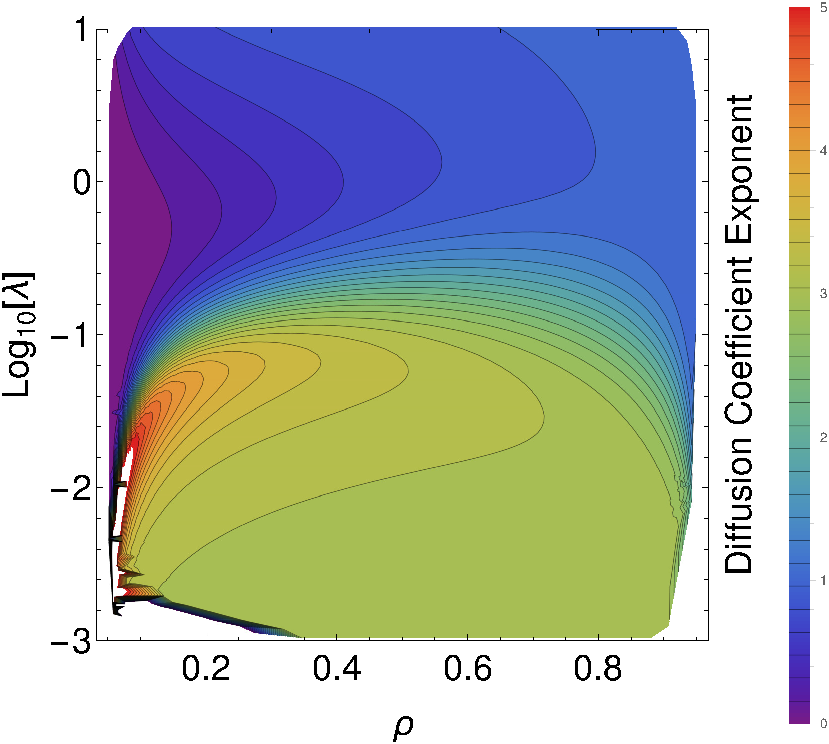
\includegraphics[width=1.0\textwidth]{TRM/images/TRMOrderParam}
  \end{center}
\end{figure}
As you can see, this order parameter does seem to nicely partition $(\rho, \lambda)$ space into two
components, divided by a region of extremely rapid change. The order parameter $\chi$ could be regarded as
some kind of susceptibility. An issue here is that it is hard to see how $\chi$'s apparent transition
will vary with system size, as $L=10$ is a very small system, and transitions only become sharp in the
limit of large systems. We could of course use it in a Monte-Carlo calculation in a larger system, but
then we have the problem that it's difficult to take meaningful derivatives of noisy data. We will leave
it, then, as a curiosity.

\section{Time-Dependent Properties of Small SPM Systems} \label{sec:TRMTimeDep}
Although we have mostly concentrated on calculating steady state properties of the SPM, it is also possible to calculate some dynamical properties. 
\subsection{The Relaxation Time for the SPM} \label{sec:relaxTime}
As we have seen, the eigenvalue with least negative real
part effectively controls the rate at which a generically-prepared system equilibrates, by acting as a lower bound on the rate of relaxation towards equilibrium. Therefore, the reciprocal of this 
relaxation rate should yield a characteristic time for convergence to equilibrium, the relaxation
time. We have computed this relaxation time for
our three standard boundary conditions in Fig.~\ref{fig:TRMRelaxTime}.
 \begin{figure}[h!]
 \caption[The dependence of the relaxation time on $\lambda$ for three sets of boundary conditions.]{\label{fig:TRMRelaxTime} 
A plot showing the dependence of the relaxation time upon $\lambda$ for a system of size $L=10$ with
boundary densities $(0.3, 0.1)$, $(0.6, 0.4)$ and $(0.9, 0.7)$. In terms of units, here we are presuming that the default diffusion rate $\tau_0 = 1 \mathrm{s}^{-1}$.
 }
  \begin{center}
 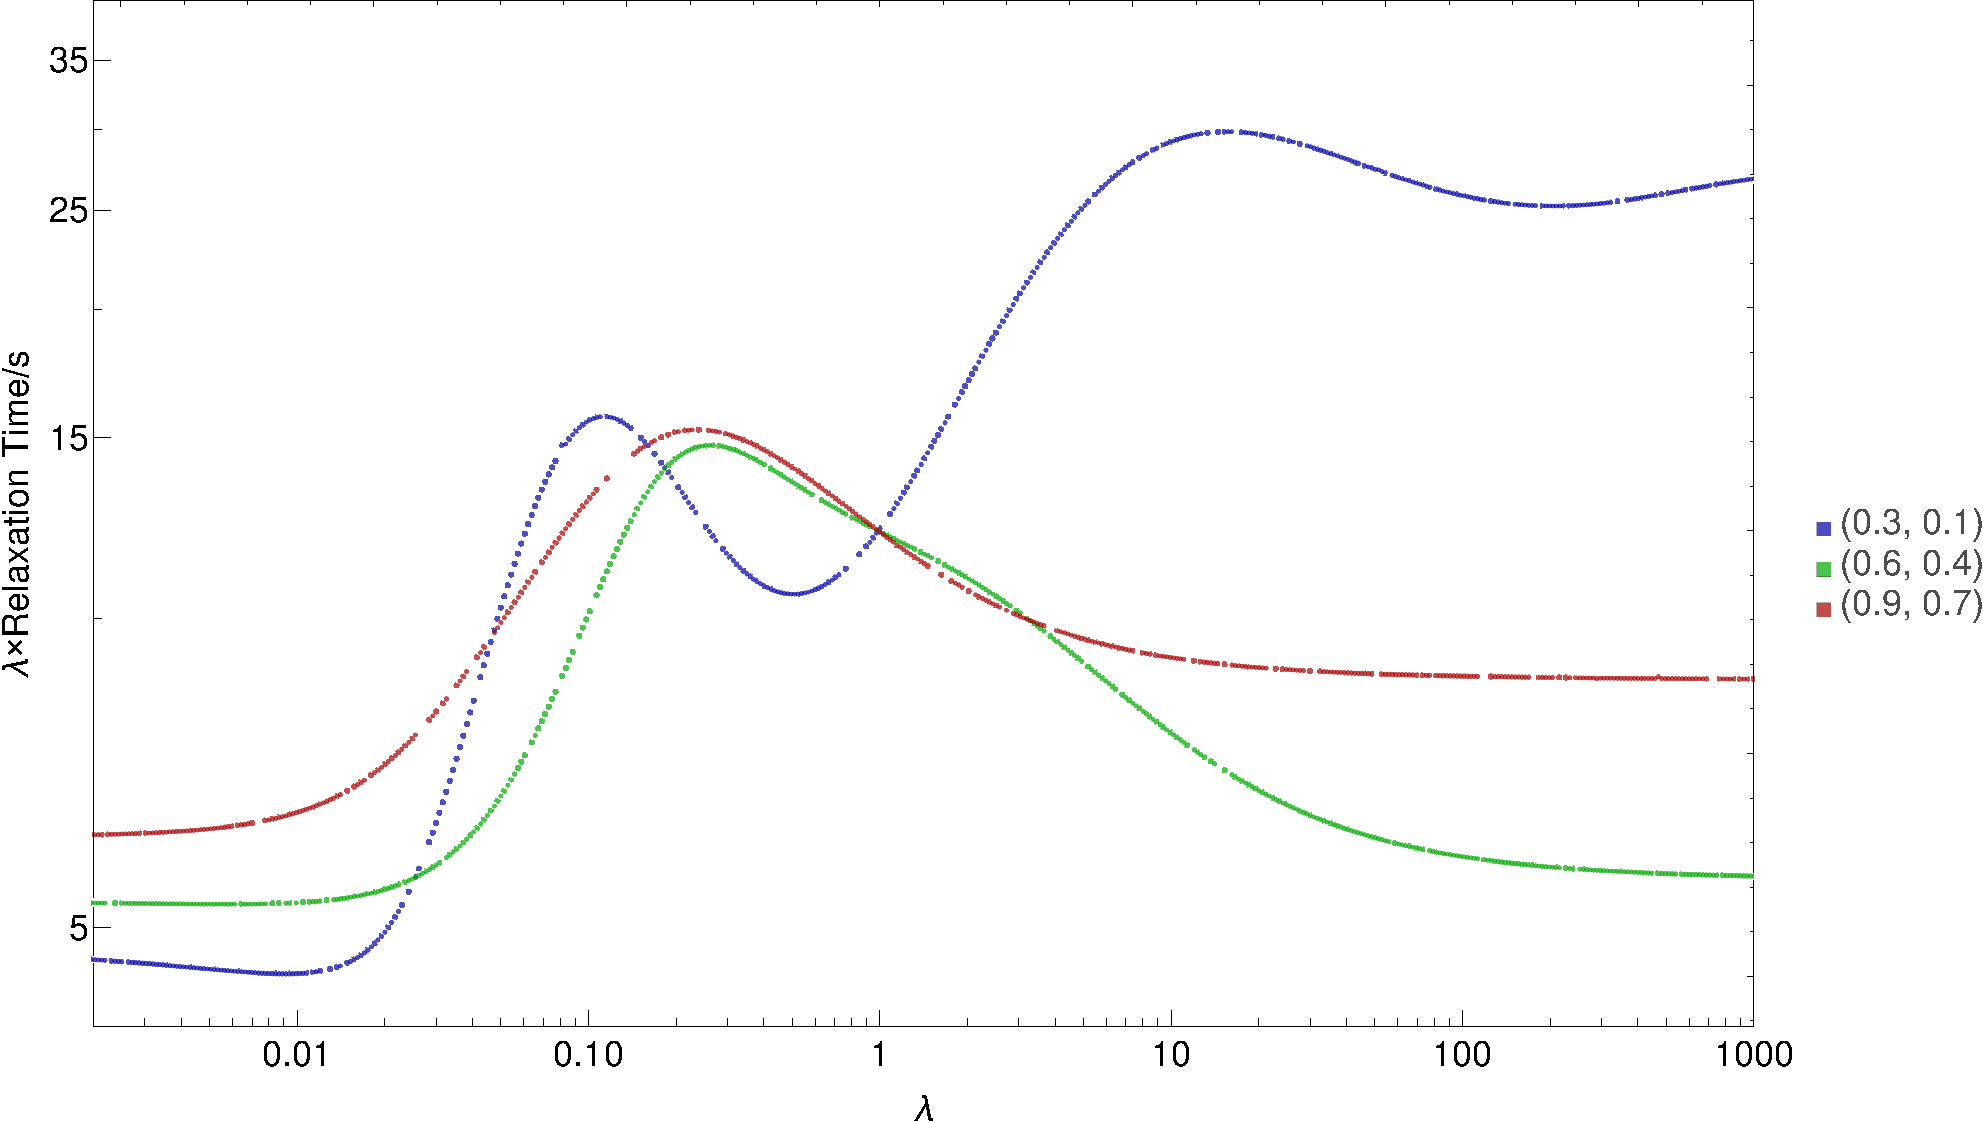
\includegraphics[width=1.0\textwidth]{TRM/images/TRMRelaxTime}
  \end{center}
\end{figure}
Notice first that we have plotted the relaxation time multiplied by $\lambda$, as the relaxation time
generally scales as $\mathcal{O}(\lambda^{-1})$. One can see why we made this choice by looking at the
extremes, where the lines are generally quite flat.

Observe that the relaxation times for large $\lambda$ are generally a little higher than for low 
$\lambda$ once the $\mathcal{O}(\lambda^{-1})$ dependence is taken into account. In particular, the
system with low densities at the boundary is much slower to relax to equilibrium than the system with high boundary densities, which in turn is slow compared to the system with medium densities. This is
presumably because the system is attempting to reach the maximal flow density we observed, $\rho = \frac{2}{3}$, and it finds it more awkward to do that the further away the furthest boundary is from
$\frac{2}{3}$.

For very low $\lambda$, the difference between boundary configurations isn't so great, and we believe
that the differences between the boundaries occur for the same reason as for the high-$\lambda$
situation, only now the system is trying to fill instead of hold at $\rho=\frac{2}{3}$. For intermediate
$\lambda$, things are less clear. At $\lambda=1$, all systems equilibrate at the same rate; other than
that, behaviour varies pretty wildly. Equilibration time is generally on the high side for
$\lambda \in (0.03, 1)$, which is where the current looks like its undergoing some kind of
transition, so this increase in relative equilibration time could be interpreted as an accumulation of
fluctuations in that regime.
\subsection{Time-Evolution of States}
Recall from Sec.~\ref{sec:TRMGeneralResults} that the Master Equation (Eq.~\eqref{eq:masterEq}) has
a formal solution given by Eq.~\eqref{eqn:formalSoln}, in which we premultiply the initial state
by a matrix exponential of the TRM. Throughout this chapter we have been making use of the fact that
the TRM is sparse in order to perform our computations. Thus, it would seem that we couldn't
investigate the time evolution of systems, as $e^A$ is in general not sparse even if $A$ is sparse,
and thus we would instantly run out of memory if we tried to compute anything.

However, the premultiplication of a vector by a sparse matrix can be performed \textit{in place},
and this is implemented by Python's routine
\newline
\texttt{scipy.sparse.linalg.expm\_multiply}. Therefore
we have been able to calculate the time-evolution of arbitrary initial distributions. By way of an
example we prepared three systems with initial uniform distributions, in which all possible 
configurations are equally likely, and then monitored how their spatial occupations varied as they
relaxed towards equilibrium (which should always occur, as discussed in 
Sec.~\ref{sec:TRMGeneralResults}). The results are displayed in Fig.~\ref{fig:TRMTimeDep}.
\begin{figure}
\caption[The time-evolution of uniform distributions to equilibrium.]{Plots of the time-evolution
of the density profiles of systems prepared with uniform distributions. These systems are of
size $L=10$, with boundary densities $(0.9, 0.1)$, $b_0=100.0$ and $\lambda= \{ 0.1, 1.0, 2.0 \}$,
going from top to bottom, respectively. The total time intervals have been adjusted to suit the 
equilibration time.} \label{fig:TRMTimeDep}
\begin{center}
 \begin{tabular}{c}
    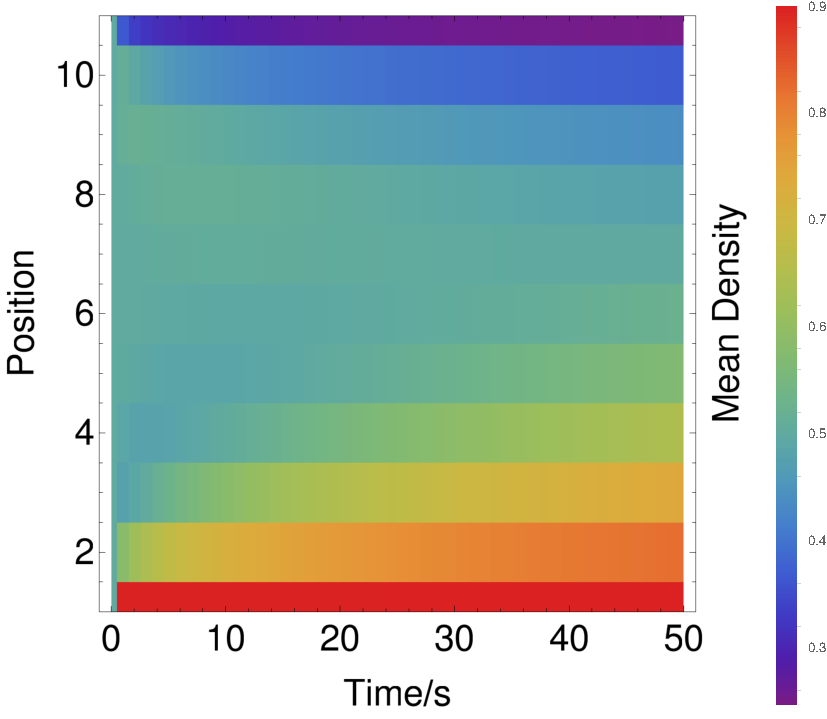
\includegraphics[width=0.6\linewidth]{TRM/images/timeSeriesl0_1}  \\ 
    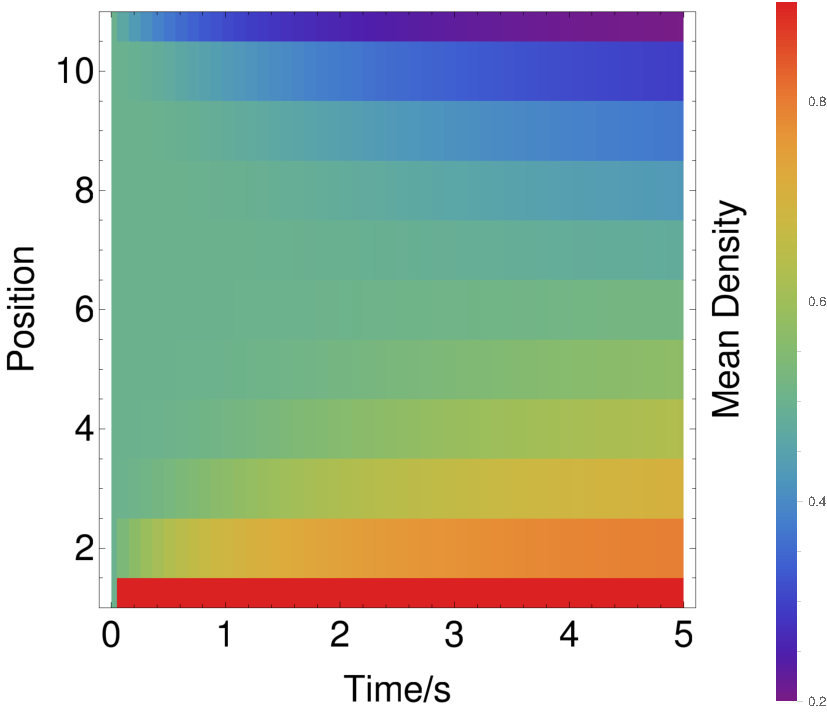
\includegraphics[width=0.6\linewidth]{TRM/images/timeSeriesl1_0}  \\
    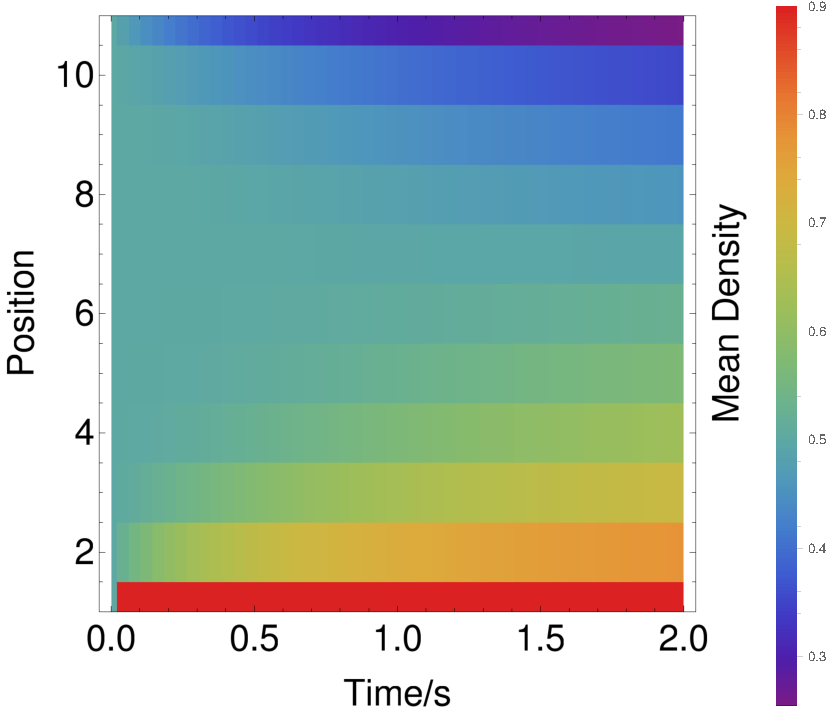
\includegraphics[width=0.6\linewidth]{TRM/images/timeSeriesl2_0}  \\
    \end{tabular}
\end{center}
    \vspace{-2em}
\end{figure}
In the plots we have included the innermost site in the boundary layer; notice that it switches to the 
``correct''
mean occupation almost instantly, which is exactly what is supposed to happen as it represents a highly
responsive reservoir. The system then gradually makes its ways toward equilibrium, starting at the 
boundaries and working inward, and the characteristic timescale over which this occurs seems to be in
line with our results from \ref{sec:relaxTime}.

Of course, this is more of a demonstration of what this method could achieve than an actually useful
result. We are quite sure that with a little effort one could use it to calculate time-dependent
spatial correlation functions,
for example, but we simply worked out how to perform TRM calculations too late in the project to be
able to use it to full effect.


\section{Conclusions}

Numerically approximating the eigenpairs of the transition rate matrix is a convenient
alternative to the use of
Monte Carlo methods for the computation of the properties of a Markovian statistical mechanics system.
When using the TRM, we sacrifice system size for accuracy, as the memory requirement for TRM
calculations scales exponentially with system size, whilst similar Monte Carlo calculations' memory 
requirements scale 
linearly. However, the TRM method avoids the
sampling issues which often emerge when attempting Monte Carlo simulations, and can yield the relevant
statistics with relative ease once the matrix computations are completed. Furthermore, we can also
investigate time-dependent properties at our convenience, which can be awkward in Monte-Carlo 
calculations as there we don't usually work with normal time.

The main reason we performed these calculations, however, is to investigate the current flowing due
to the boundary conditions. We found that the MFT prediction that the currents drops to zero or becomes 
negative below a critical $\lambda$ (depending upon boundary conditions) does not seem to be correct;
however, we have found that the scaling of the current does seem to undergo some kind of transition,
from  $J \propto \lambda$ for large $\lambda$ to $J \propto \lambda^3$ for small $\lambda$.
This is something which we can
investigate further using Monte-Carlo methods on larger-scale systems, and we will do this in the next
chapter.

%\chapter{Monte-Carlo Simulations of the SPM} 
\label{sec:numerics}
We now have numerical results for SPM systems using TRM analysis; however, this only allows us to study
relatively small systems. In order to study larger ones, we have used Monte-Carlo methods. In this
chapter, we will discuss the methods we used, the results they yielded, and their meaning, with 
particular emphasis on what they tell us about the suspected transition between low and high-$\lambda$
behaviours.
\section{Numerical Simulations of Continuous-Time Markov Processes}
Here we will discuss the theory behind the Monte-Carlo methods used to simulate continuous-time Markov
processes. We will assume throughout that we have the computational means to produce pseudorandom
floating-point numbers in a way which which closely approximates the uniform real distribution over $(0, 1)$.
\subsection{Purpose of Monte-Carlo Methods}
We should first really describe what we mean by a Monte-Carlo method. In essence, Monte-Carlo methods
refer to numerical routines in which we attempt to characterise an unknown distribution, generated 
via known rules, by using
pseudorandom numbers in order to produce sample data which is hopefully faithful to the original 
distribution, at least in terms of the statistics we are trying to calculate. A good example of a
commonly-used Monte-Carlo method in Physics is the Metropolis-Hastings algorithm, which in its original
form is used to calculate statistics for equilibrium statistical mechanics systems.

In our situation, we wish to be able to mimic a continuous-time discrete-state Markov process.
As we saw in Chap.~\ref{sec:transRateChapter}, the state space for a TRM system of size $L$
scales as
$\mathcal{O}(2^L$); thus we quickly run out of size if we try to consider exact probability distributions, which correspond to
vectors in $\mathbb{R}^{L^2}$. We can, however, store individual configurations, which only occupy
$\mathcal{O}(L)$ space. Therefore, we need to find a way to produce trajectories through the discrete
state space which sample the actual space of system trajectories well enough to allow us to access the
statistics we want. Of course, there isn't a unique ``best'' way to do this. We have considered two
contrasting methods, which differ primarily in the way in which they convert the original continuous 
time into discrete steps which we can use in an algorithm.

\subsection{Evenly-Spaced Timesteps} \label{sec:evenTimesteps}

If we wished to numerically approximate an ODE system, one might use the Euler forward or 
Runge-Kutte methods. These both involve discretising time simply by dividing it into evenly-sized
pieces, and then converting the ODE into a discrete form by using finite differences to
approximate derivatives. We need to be careful to choose a small enough timestep for
the approximation to the derivative to remain good, but otherwise it is a very simple and 
effective approach.

We can do a very similar technique with continuous time Markov processes. In our SPM system,
if we ignore the boundaries, there are two rates, $1$ and $\lambda$, and our system is 
homogeneous. Let us represent the system with a binary array of length $L+2$, with $L$ sites for the bulk
and a site each representing the boundaries. Therefore, in order to simulate the action of the SPM as
defined in <reference to appropriate section in
introduction>, we can use the following recipe:
\begin{enumerate}
 \item \textbf{START}. Advance time by $\Delta t$. Pick a site, which we will call
 Site,
 (of which there are $L+2$) at random. If the site chosen is one of the boundaries with density $\rho$,
 reset the site to be occupied with probability $\rho$ and unoccupied with probability $1-\rho$.
 \item If Site is occupied, pick one of the two adjacent sites, which we will call Target, at random with equal probability.
 This will be the site we attempt to move into. If Site is not occupied, go back to \textbf{START}.
 \item \textit{If Site is not on the boundary}: If Target is occupied, go to \textbf{START}. Otherwise, consider the other adjacent site,
 which we will refer to as Rear. If Rear is empty, move the particle in Site into Target 
 randomly with
 probability $\frac{1}{1+\lambda}$; otherwise, move the particle with probability
 $\frac{\lambda}{1+\lambda}$. Return to \textbf{START}. 
 \newline \textit{If Site is on the boundary}: If Target is outside the system, go to \textbf{START}.
 If Target is occupied, go to \textbf{START}. Assign an occupation value for Rear randomly, occupied
 with probability $\rho$, unoccupied with probability $1-\rho$, where $\rho$ is the density of the relevant
 boundary. Now, if Rear is empty, move the particle in Site into Target 
 randomly with  probability $\frac{1}{1+\lambda}$; otherwise, move the particle with probability
 $\frac{\lambda}{1+\lambda}$. Return to \textbf{START}.
\end{enumerate}
We define $\Delta t$ via 
\begin{equation}
 \Delta t = \frac{\tau_0}{L (1+\lambda)}.
\end{equation}
In terms of the algorithm's correctness at producing reasonable trajectories, we simply need note that
the rates at which particular transitions should occur are in the correct proportions, and that the boundaries result in the correct densities in equilibrium;
then, we just need
to verify that the rate at which free particles move is the correct one in absolute terms, which it is,
and we're done. 

For Monte-Carlo methods, we generally rate their performance by the amount of computational
power required to explore a given amount of the probability space. In methods in which we
are exploring this space by advancing though time (and invoking ergodicity) we desire methods
which move us quickly through time whilst maintaining good sampling and performing little computation.

The advantage of this method is that it is very simple; thus, there aren't too many opportunities
for error when writing the code, it uses very little memory (all calculations can be performed
in-place), and each iteration should be very fast as there are very few overheads. It should also
produce trajectories which are good samples of the original probability distribution we are 
trying to replicate.


If $\lambda$
is close to $1$, the probability of rejection (i.e. a step which results in no overall change to
the system) is $\sim\frac{1}{2}$, and this is the situation in which the algorithm really shines; similarly
it also performs well for large or small $lambda$ if the system density is very high or very low
respectively. For extreme $\lambda$ in general however, performance drops off considerably, as
we are often performing lots of calculations and advancing time very little, and thus not seeing
much of the distribution simply because we aren't moving much.

We could have made this code marginally more efficient by making the more likely moves certain, and
correspondingly adjusting the timestep size $\Delta t$ to account for this; however, this only
improves efficiency by a factor of around $2$ , whilst making the code more complicated, so as
we only used this method to verify the results of our main code it didn't seem worthwhile.
It is possible for us to get
around this issue by advancing time in a variable fashion, although this comes at the cost of
a little more computation per iteration.

\subsection{The N-Fold Way, or Gillespie Algorithm} \label{sec:nFoldWay}
A popular way to produce trajectories for a continuous-time Markov process is the N-Fold Way, also known as the
BKL or Gillespie Algorithm~\cite{Bortz1975, Prados1997, voterKMC}. It evolves us through time as follows:
\begin{enumerate}
 \item \textbf{START}: Make a list of all states which can be transitioned to in a single move from the 
 current state, and the associated rates at which this occurs.
 \item Weight each successor state by the transition rate into it, and then select a successor state by
 random selection from a uniform distribution over the weighted possible successors. Change the system
 state to the chosen successor. \label{weightingChoose}
 \item Now advance time by an increment chosen from an exponential distribution whose decay rate 
 is the sum of all of the rates of the possible transitions to a successor. Go back to \textbf{START}. \label{timestepChoose}
\end{enumerate}
Now we just need to supply the rates <from introduction> that define the SPM, along with some additional rates describing processes at the boundary. Specifically, we use the method described 
in~\ref{sec:CTMPBoundaries} to do this, whereby we have a double layer of ``blinking'' boundary sites
and sites in the internal layer undergo the same transitions as in the bulk. However, unlike in our TRM
calculations, we should not set the incoming and outgoing rates to be extremely high, as then these rather
trivial processes come to dominate the calculation and cause the timesteps to be on average extremely small, wasting our computing time. Instead, we set them to
be proportional to the geometric mean of $1$ and $\lambda$, and thus in the language of~\ref{eq:blinkRates}
this corresponds to setting $B_0 = \sqrt{\lambda}$. This way the boundaries refresh often, but not too
often, and should still act as suitable reservoirs, which we can test by comparing small systems with 
Chapter~\ref{sec:transRateChapter} and comparing with code in Sec~\ref{sec:evenTimesteps}.

We will get into the fine details about how the software we use implements KMC in Sec.~\ref{sec:kmcLib}.
Let us first discuss how we obtain the required probability distributions using the uniform distribution
on $(0, 1)$, $U(0, 1)$:
\begin{itemize}
 \item We can randomly choose the successor state required in step~\ref{weightingChoose} by
 creating a list of weighted partial sums. If the transition rate from the current state the $i^\mathrm{th}$
 potential successor state is $k_i$, then let us define $k_\mathrm{Tot.} = \sum_{i}^n k_i$, 
 where $n$ is the
 number of potential successors. Create the list of partial sums via $s_i = \sum_j^i k_j$, then generate
 the random number $u = r k_\mathrm{tot}$ where $r$ is drawn from $U(0, 1)$. We can then use a binary
 search to find $i: s_{i-1} \le u \le s_i$, and then this $i$ indicates the successor state which has been
 chosen. This process is illustrated more visually in Fig.~\ref{fig:weightChoice}.
 \item In step~\ref{timestepChoose}, we need to generate random numbers in an exponential distribution
 with decay rate $k_\mathrm{tot}$. We can do this by generating $r$ from $U(0, 1)$, and then 
 $w = -\frac{1}{k_\mathrm{tot}} \log{r}$
 follows the desired distribution.
\end{itemize}
\begin{figure}[h!]
 \caption[Illustration of the method for choosing successor states in the n-fold way.]{\label{fig:weightChoice} 
 An illustration of the suggested method for choosing a successor state in the n-fold way. Reproduced
 from~\cite{voterKMC}.
 }
  \begin{center}
 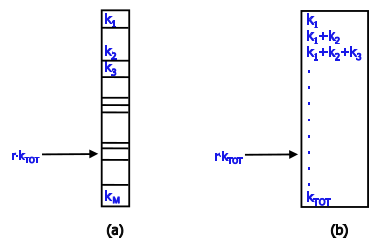
\includegraphics[width=0.7\textwidth]{numerics/images/nFoldWayRates}
  \end{center}
\end{figure}

I will defer to Voter (see in particular Sec. 5 of~\cite{voterKMC}) for the ``proof of correctness'' of the
method. The primary advantage of this method is that we are certain to advance time every step, so we are
not potentially
``wasting'' steps as
when we use even 
timestepping; this comes at the cost of having to compute which transitions are possible from the current
state. For our SPM, a given state has $\mathcal{O}(L)$ possible transitions, thus the time complexity
of a single timestep is $\mathcal{O}(L)$; note that our method with evenly-spaced timesteps has constant
time complexity, but the size of each timestep scales as $\mathcal{O}(L^{-1})$; thus we're not actually
losing as much as it appears by using variable timesteps. Furthermore, there is the possibility that the
process by which we calculate which transitions are possible could be performed in parallel, and so
the walltime cost of a single timestep in the n-fold way can end up comparatively cheap. The process of
choosing a successor state once the options are found involves performing the equivalent of a search, and
therefore takes $\mathcal{O}(\log{L})$ time and so should be insignificant.


\section{Implementation of Monte Carlo Methods}
\subsection{Our Implementation of a Metropolis-Hastings Algorithm with Evenly-Space Timesteps}
We have written a Fortran code which implements the algorithm in Sec~\ref{sec:evenTimesteps}. This is
stored in <location of code>. This programme initialises the system to have a particle density
equal to the average of the two desired boundary densities, and then proceeds in a manner extremely
faithful to the simple accept/reject algorithm.


\subsection{\texttt{KMCLib}} \label{sec:kmcLib}
The vast majority of our Monte-Carlo calculations have been performed using the n-fold way, described in
Sec.~\ref{sec:nFoldWay}. This is implemented for continuous-time Markov processes on crystalline lattices
(of which the SPM is an example) in a software package called \texttt{KMCLib}, documented 
at~\cite{leetmaa2014KMCLib} developed by Dr Mikael Leetmaa.

\texttt{KMCLib} is a Python-wrapped C++ package. This means that the frontend, where one specifies the
system to be simulated, the data to be recorded, and how the simulation is run, is written in a Python
script; then, when this script is run, it executes C++ code in order to represent the system and
actually carry out the desired operations. Furthermore, \texttt{KMCLib} can perform calculations in
parallel if so desired. Whilst there exist examples~\cite{hoffmann2014kmos, spparks} of kinetic
Monte-Carlo codes other than \texttt{KMCLib}, we chose to use that one due to our familiarity with all
of the languages involved, and preference for a Python frontend.

Of course, setting up different calculations which vary different parameters or measure different things
require different scripts. Going through every script we wrote individually would cause this thesis
to be around twice as long and three times more dull; therefore we have instead chosen to focus
upon a single set of codes designed to perform a particular calculation, which we have annotated and 
included here <location>; the intention is that a reader wishing to reproduce any of our results could do
so by performing a few simple modifications to the code listed there. A more comprehensive codebase is
stored at <location>, but this is sparsely annotated working code, and so might not be very helpful.

A code which provides Python input for \texttt{KMCLib} is contained within 
\texttt{concFlow.py}. This script takes in several command line inputs. These provide the parameters for
a simulation of the SPM, with the desired value of $\lambda$, system size and boundary conditions. It 
then sets up the representation of the system configuration and the means to enumerate possible
transitions and their associated rates, as is necessary to implement the n-fold way.
The initial configuration is generated by randomly inserting particles into the system until its density
is equal to $\frac{1}{2}\left(\rho_0 + \rho_L \right)$; we then perform $N_{\mathrm{eq}}$ KMC steps in order to 
equilibrate the system (in case the initial configuration we chose was highly deviant from the norm
for the prescribed parameters). The actual measurements are performed by time-averaging values for system
quantities (e.g. the number of particles entering the system at one end) over $N_{\mathrm{meas}}$ steps,
relaxing the system (in other words, performing steps but taking no measurements) for $N_{\mathrm{req}}$ steps,
and then repeating this process $N_{\mathrm{pass}}$ times. This way, we can generate $N_{\mathrm{pass}}$ time-separated 
observations of, say, the total current through the system, and because we are relaxing the system 
between measurement runs we should not have to worry too much about the results being unduly correlated
with each other, (assuming we set $N_{\mathrm{req}}$ high enough).
Thus, we supply \texttt{concFlow.py} with the following parameters as 
command line inputs:
\begin{enumerate}
 \item The particle reservoir concentration at one end of the domain, $\rho_0$.
 \item The particle reservoir concentration at the other end of the domain, $\rho_L$.
 \item The value of $\lambda$ to use in the simulation.
 \item The system size, $L$.
 \item The interval between measurements performed by the analysis
 routines, $N_{\mathrm{anal}}$. This should be set to $1$ in order to measure the current.
 \item The number of equilibration steps, $N_{\mathrm{eq}}$.
 \item The number of analysis steps per pass, $N_{\mathrm{meas}}$.
 \item The number of reequilibration steps per pass, $N_{\mathrm{req}}$.
 \item The total number of passes, $N_{\mathrm{pass}}$, which give separate
 sets of observations, performed during this calculation.
 \item A timescale, $\delta t$, which indicates how often to evaluate,
 and to what accuracy to record, times, when measuring the number of 
 particles in the system. We recommend that this be small compared to the expected KMC timestep size.
\end{enumerate}

In terms of the output of the code, it produces a short file summarising the input parameters,
some trajectory dump information (usually redirected to \texttt{/dev/null} in order to save hard
memory, which is often in short supply), as well as data taken by measurement routines. We nominate,
from a suite of possible routines, which measurements we would like it to take during analysis phases.
Note that in our calculations, we do not use any quantity's value during particular KMC steps;
rather, we always average our quantities over some amount of time. This is partly because some of the
quantities we are interested in do not really have any value during a single timestep (e.g. the flux of
particles through one of the boundaries), and also because the amount of time spent in particular
configurations could potentially vary wildly between configurations. The amount of time spent in a
particular configuration in the n-fold way is drawn from an exponential distribution with decay rate
$k_{\mathrm{tot}}$, as we saw in Sec.~\ref{sec:nFoldWay}; thus, one could easily imagine a
situation in which the transition time varies wildly. For example, say we have a system with very low 
$\lambda$. If this system was quite full, there would be few transitions possible, and those possible
transitions would likely occur with low rates, therefore the KMC timesteps would tend to be very long.
However, later during the same simulation we could find ourselves in a situation where the system is
less full, and so more transitions can occur, and generally with much higher rates, leading to much
shorter timesteps. Thus, we shouldn't really treat particular quantities derived from these 
configurations with an equal footing, as the amounts of time the system spends in each are so very 
different.

The precise nature of our time-averaging depends a little on the measurement in question. The types
of measurements we usually perform are the following, where $T$ is the total time elapsed during
our $N_\mathrm{anal}$ step measurement run:
\begin{itemize}
 \item \textbf{Current} We count the total number of particles which enter or leave a given boundary
 over the course of the measurement run. Let the number of particles entering and 
 exiting at the $0$ boundary be $u_0$ and $w_0$ respectively, and likewise for the $L$ boundary with
 $u_L$ and $w_L$. Then
 \begin{equation}
  J = \frac{u_0+w_L-u_L-w_0}{2T}
 \end{equation}
should be a good estimate of the total current through the system during that time period.
\item \textbf{Block Size Distribution} In one dimension, we can look at a configuration and count how
many contiguous runs (``blocks'') of particles there are of different sizes (e.g. size 1 means a single
particle sandwiched between adjacent vacancies). We can find the distribution of block sizes, weight it
by the length of the associated KMC timestep, and then add this to a running total. If we do this over
our $N_\mathrm{meas}$ analysis steps and then normalise, we can build a histogram of the block sizes
during that time period.
\item \textbf{Particle Density} Similarly, we can count the total number of particles in the system,
weight it by the length of the KMC timestep, and then use this to build another histogram of the
system particle density. By keeping track of particles entering and leaving the system, it would be
possible to code this very efficiently to take $\mathcal{O}(1)$ time; however, as our routine to detect
block sizes scans through the system and counts as it goes along, we have just opted for a simple
$\mathcal{O}(L)$ scan of the whole system for our density measurement as well.
\end{itemize}
Using these analysis routines, we can generate time-averaged values for particle density histograms,
the block size distribution and the current. By calculating $N_\mathrm{pass}$ separate instances of 
these observables, we get $N_\mathrm{pass}$ samples from the relevant distributions, and from there
we can probe the statistics of these variables.


\subsection{Managing \texttt{KMCLib} Calculations in Parallel} 
Of course, it is one thing to have a code which can run on a laptop to produce the output of a 
particular simulation over the course of a day. It is quite another undertaking to run thousands of
separate calculations in order to map out parameter spaces and compute derived quantities such as the
diffusion coefficient. 

We have been running our calculations on Edinburgh University's \texttt{Eddie3} computing cluster.
This machine does not boast the high level of processor interconnection density of \texttt{ARCHER}
or the extremely high working memory of \texttt{DiRAC}; however, for the purposes of our calculations
it turns out that we need neither. The KMC algorithm only stores a single state of the system under
simulation at any given time, therefore its space complexity only scales as $\mathcal{O}(L)$.
Furthermore, whilst \texttt{KMCLib} can be run in parallel mode in order to take advantage of
a multithreaded environment, this isn't actually an advantage when we wish to run very large numbers
of separately-parametrised calculations, as the total amount of CPU time required remains the same,
whilst incurring additional overheads associated with parallelism.
Therefore, we have used a single-threaded environment for all of the calculations featured in this
thesis.

In order to set up a batch of calculations, we use the following procedure, implemented by the codes
stored in \texttt{kmc/1d/} within <location>:
\begin{enumerate}
 \item Create a batch of input files, in the subdirectory \texttt{jobInputs/}. In our setup, we
 require that files titled
 \texttt{testInput.}$i$ are generated, with $i \in [1, n]$ where $n$ is the total number of 
 calculations to be performed. These input files are typically generated by a code such as 
 \texttt{lambdaFlucCreator.py}; parameters which determine the overall structure
 of the system (e.g. $L$, the system size) will usually be held constant across calculations, whilst
 parameters such as the stickiness or the boundary densities will be varied between them. These input files contain a single line of code, which will be appended to \texttt{python } and called in the command line.
 \item In order to actually perform the calculations, we submit them as \texttt{gridengine} batch
 jobs. We  run the script \texttt{kmcSubmit.sh}, which submits the nominated tasks whose input
 files are in \texttt{jobInputs/}, using the scripts \texttt{kmcJobArray.sh} and 
 \texttt{initKmc.sh} for intermediate steps. \texttt{kmcSubmit} is also the place where we specify
 calculational parameters, such as maximum memory usage, maximum runtime, etc; these will be taken
 into consideration by \texttt{gridengine} when it comes to scheduling these calculations, so it
 is important that the maxima be relatively tight upper bounds, otherwise the calculation priority
 will be extremely low, assuming that the cluster in question is being simultaneously used for many other
 calculations.
 \item The jobs will then be executed, in their own time. The results will be placed in the location
 nominated by the input files.
 \item Once the run is complete, and the data has been saved, we are then ready to process it into a
 more useful format, in our case a data file which can be interpreted by Mathematica, the programme
 we used for most of our analysis and graphing. This is done using a script such a 
 \texttt{lambdaPostProc.py}. Note that such
 a script needs to be able to handle the fact that data may not be produced for some of the 
 calculations (around 5\% in our experience). The most likely source of the
 problem seems to be an issue with type conversion between Python and C++, which only seems to 
 become a significant issue in larger calculations.
\end{enumerate}
Note that throughout our calculations, we have stored data in a human-readable format, instead of
in a more compressed binary format. This is because we believe that the benefit of having a 
human-readable format, and therefore a much greater ability to look through data and check the 
output, outweighs the associated memory cost (around a factor of $10$ or so), 
especially given that any memory reduction attained due to such a format change wouldn't alter
what was feasible in terms of what we can afford to store.


\section{1D Calculation Results} \label{sec:1dMonteCarlo}
Most of the calculations we have performed are for the $1$-dimensional version of the SPM. As we 
have already performed calculations relating to $1$D behaviour in Chaps.~\ref{sec:analChap}
and~\ref{sec:transRateChapter}, we already have results which can be compared directly to our
Monte Carlo calculations; thus, we will be plotting them together wherever we feel it is
appropriate.

In terms of what to calculate, we can use our previous calculations to motivate our future ones.
Using Monte Carlo, we can calculate the quantities we already investigated, such as current and 
particle density. In addition, we can also look at the time-evolution of particular configurations,
to gain insight into the mechanisms by which particles are transmitted during flow. This is
something our MFT says essentially nothing about, and our TRM calculations are too small to see 
anything meaningful in this regard.

\subsection{Flow Patterns} \label{sec:flowPatternVis}

First, let's talk about these flow patterns. Of the two methods available, we have only implemented
the visualisation of flow using the KMC calculations. This is because the n-fold way produces
a more ``realistic'' trajectory for the SPM, in the sense that the trajectory is an exact 
reproduction of the behaviour of the continuous-time Markov system; our other method, the simpler
accept-reject algorithm, should reproduce correct behaviour when long-term time averages are taken,
but might behave badly over small times. For example, in this method, there is a \textbf{minimum} timescale
over which \textbf{any} particle can move, which is not the case for KMC, with its random timestepping.

Whilst this random timestepping makes for a more formally correct trajectory, it does make it a
little more difficult to produce visualisations of particle trajectories. Our method for overcoming
this is as follows:
\begin{enumerate}
 \item Calculate a trajectory, with whatever choice of system parameters we like. The most 
 condensed way to do this in terms of hard memory during calculation runs is to keep track of which
 slots' occupancies change state at each 
 timestep, and retaining the timestamp of each timestep.
 \item From this occupancy data, we can use linear interpolation in order to assign a continuous
 occupancy variable to all sites at all times. Between timesteps, all sites not directly involved
 with a transition would have an occupancy of $1$ or $0$, and those involved in the transition
 would smoothly switch from occupancies of $0$ to $1$ and vice-versa.
 \item We can now make a new, evenly-stepped grid of space and time where we use even timesteps.
 We can integrate the interpolated KMC data over the time spacings of the new grid in order to
 find average occupations over the specified timeframe. 
\end{enumerate}
Thus, we can produce a spacetime diagram which shows the motion of particle density through the 
system over time. Clearly this method depends upon supplying a timescale $\delta t$ over which we
perform our averaging; a large $\delta t$ will ignore most of the specifics of the motion, whereas
a very small value will reveal a system in which only one particle is moving at any given time.

\subsubsection{Flow Visualization for Sticky Particles} \label{sec:1DStickyPlots}
We have performed calculations which illustrate the behaviour of an SPM system in $1$ dimension, displayed
in Fig.~\ref{fig:1DStickyPlots}. These plots were generated by simulating SPM systems with $L=512$
and boundary conditions $(\rho_0 , \rho_L) = (0.75, 0.25)$, with $\lambda \in \{ 0.05, 0.15, 0.35 \}$.
We simulated over differing numbers of KMC steps, $N_\mathrm{steps}$, in the end performing
$N_\mathrm{steps} \in \{ 8192, 262144, 2097152, 8388608 \}$ steps respectively. Once the data was collected,
we could lookup the total elapsed time in each simulation, $T$, and then divide that time by $512$ in order
to obtain a discretization timescale $\delta t$, as required by our method for visualising flow patterns
described above in~\ref{sec:flowPatternVis}. In this way, we can visualise what the flow looks like over
different timescales for different values of $\lambda$. Note that the average size of a KMC step \textbf{does}
depend
implicitly on the value of $\lambda$; thus, the timescales portrayed in Fig.~\ref{fig:1DStickyPlots}
are not consistent between the plots, as the timesteps are multiples of lengths 
$\sim \{ 6, 2, 1 \}\times 10^{-2} \mathrm{s}$ for $\lambda \in \{ 0.05, 0.15, 0.35 \} $ respectively. In
all of these plots, dark tones represent low time-averaged particle occupation, whilst light tones
represent high time-averaged particle occupation.
\begin{figure} \caption[The flow pattern of sticky particles in $1$D]{Spacetime plots of the particle flow
in 1 spatial dimension, as described in~\ref{sec:1DStickyPlots}. In each case, the $x$-axis represents time
and the $y$-axis space. The higher-density boundary is the one at the top of each image. Dark tones 
indicate low particle density, light tones high.} \renewcommand{\arraystretch}{-0.5}
\label{fig:1DStickyPlots}
\begin{center}
\begin{tabular}{c @{\hskip -0.5em} c| c @{\hskip -0.5em} c @{\hskip -0.5em} c} 
 & $\lambda$ & 0.05 & 0.15 & 0.35 \\
 $\frac{N_\mathrm{steps}}{8912}$ & & & &  \\ 
 \hline
 \rule{0pt}{0.1\normalbaselineskip} & & & & \\
 \raisebox{5em}{1}  &  & 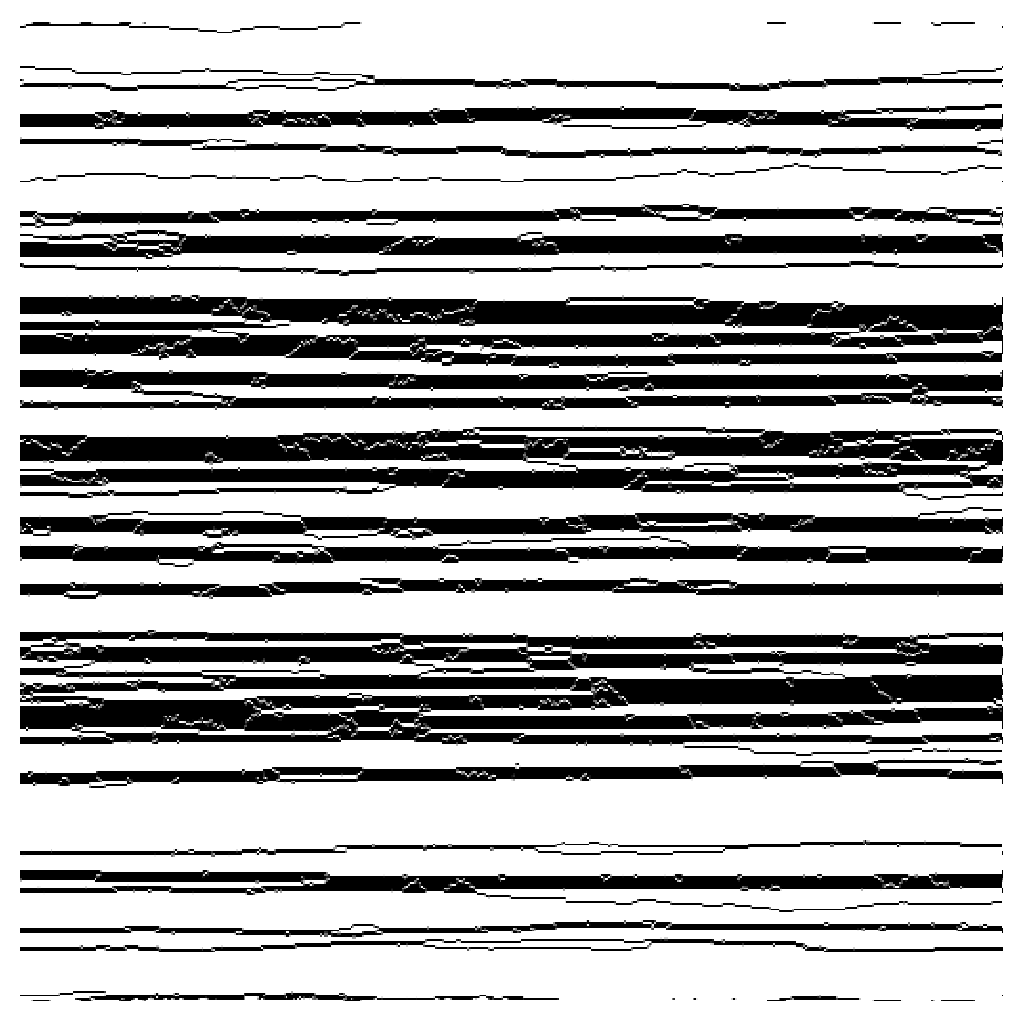
\includegraphics[width=0.31\linewidth]{numerics/images/stickyParticleFlows/flowImpL0p05T1p32.png}
 & 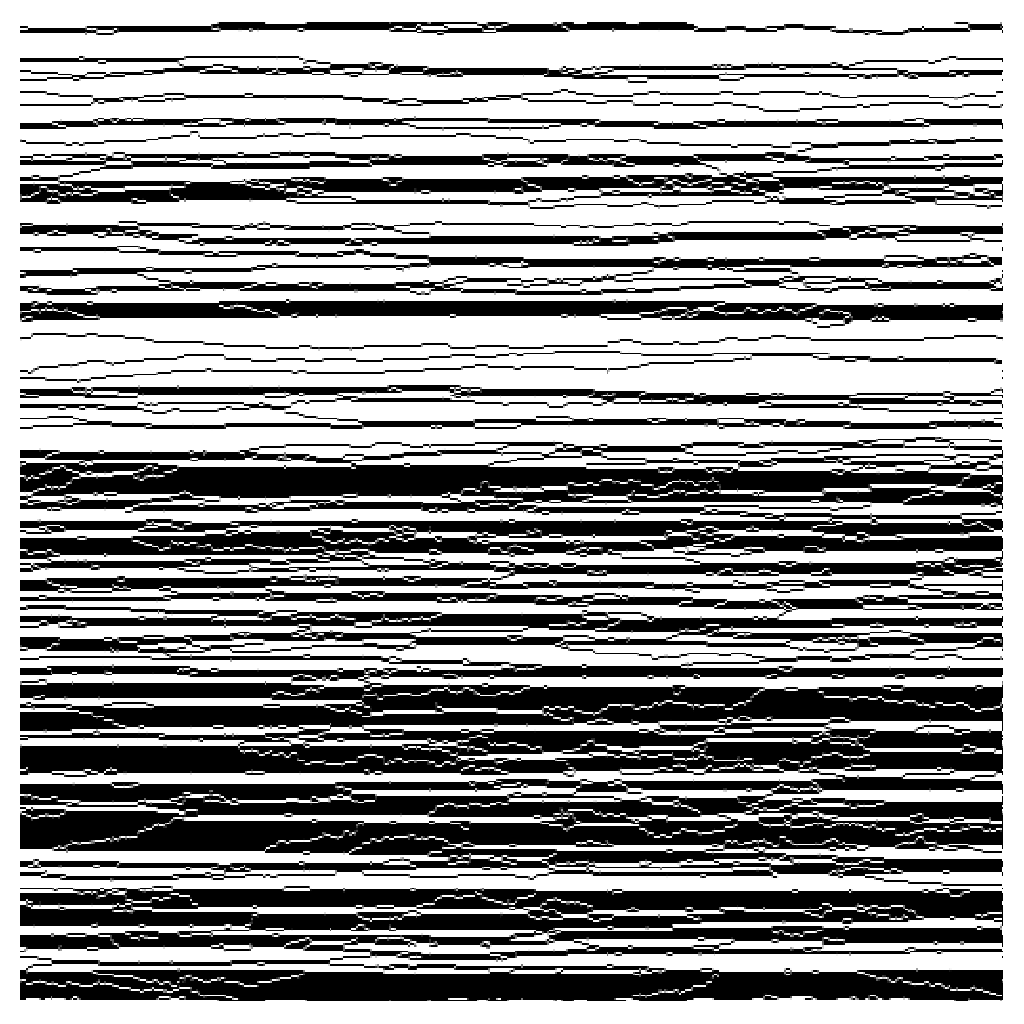
\includegraphics[width=0.31\linewidth]{numerics/images/stickyParticleFlows/flowImpL0p15T1p32.png} 
 & 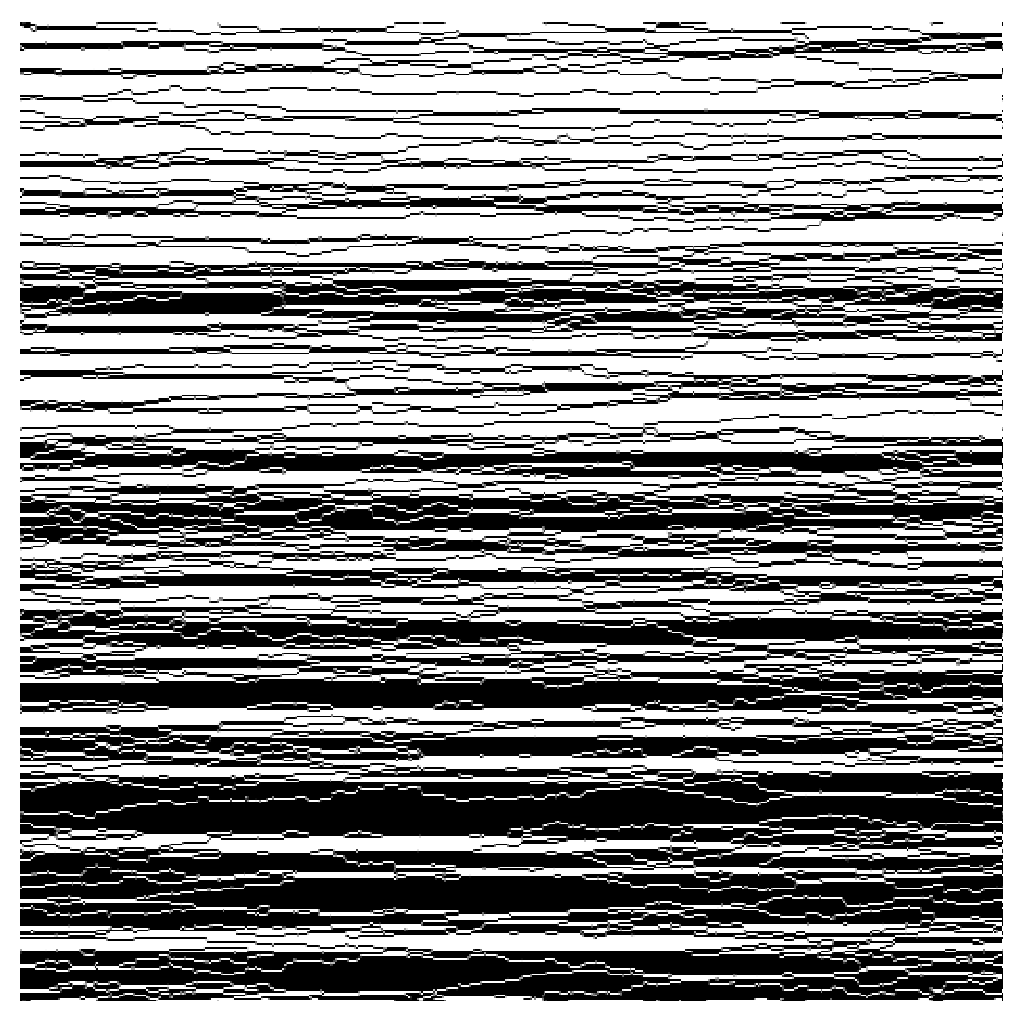
\includegraphics[width=0.31\linewidth]{numerics/images/stickyParticleFlows/flowImpL0p35T1p32.png} \\ 
\raisebox{5em}{32} & & 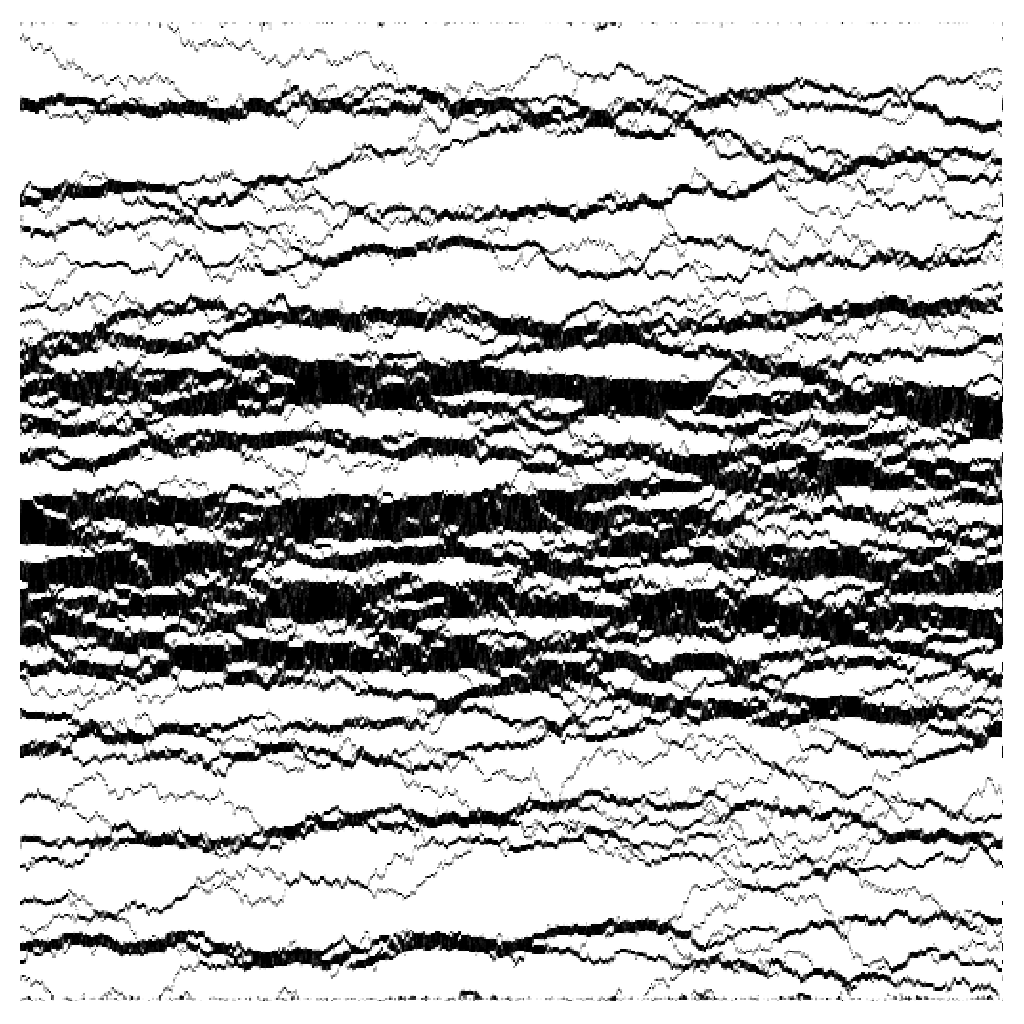
\includegraphics[width=0.31\linewidth]{numerics/images/stickyParticleFlows/flowImpL0p05T1p0.png} 
 & 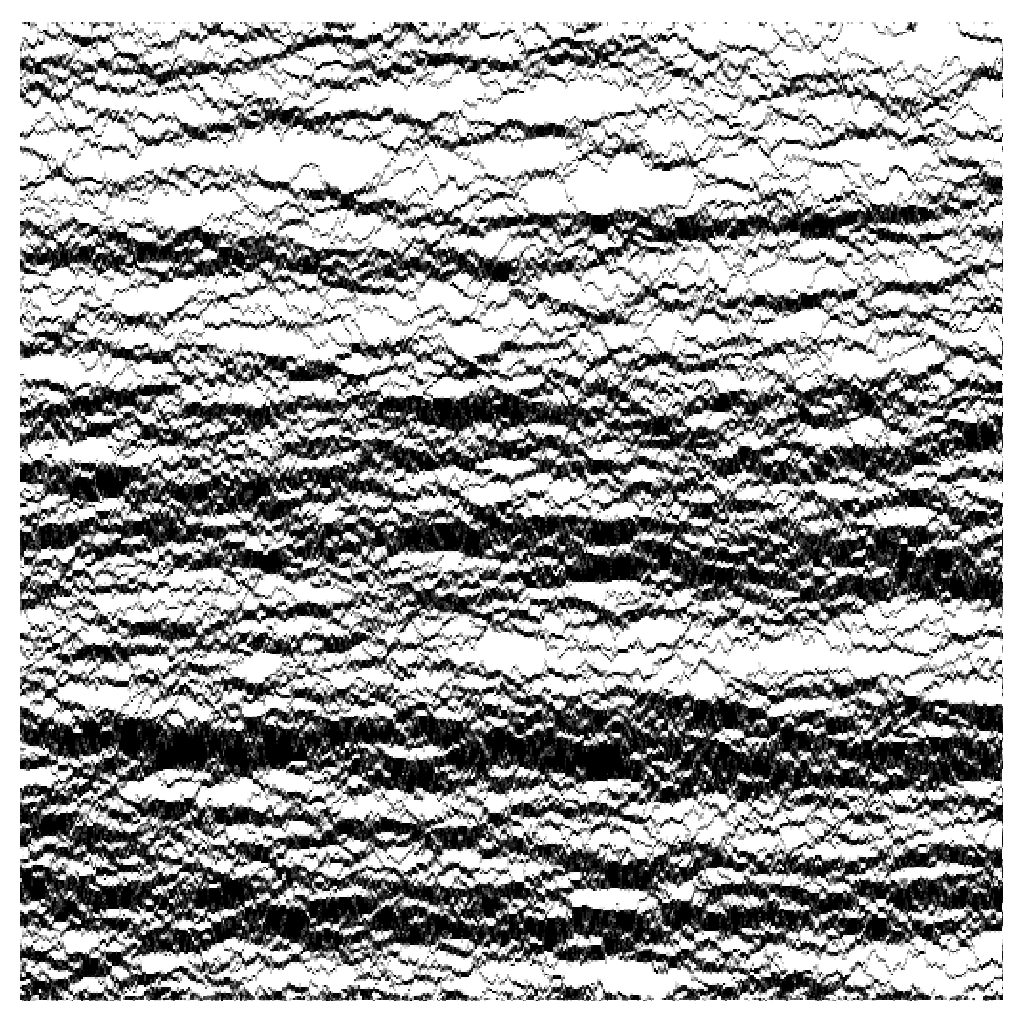
\includegraphics[width=0.31\linewidth]{numerics/images/stickyParticleFlows/flowImpL0p15T1p0.png} 
 & 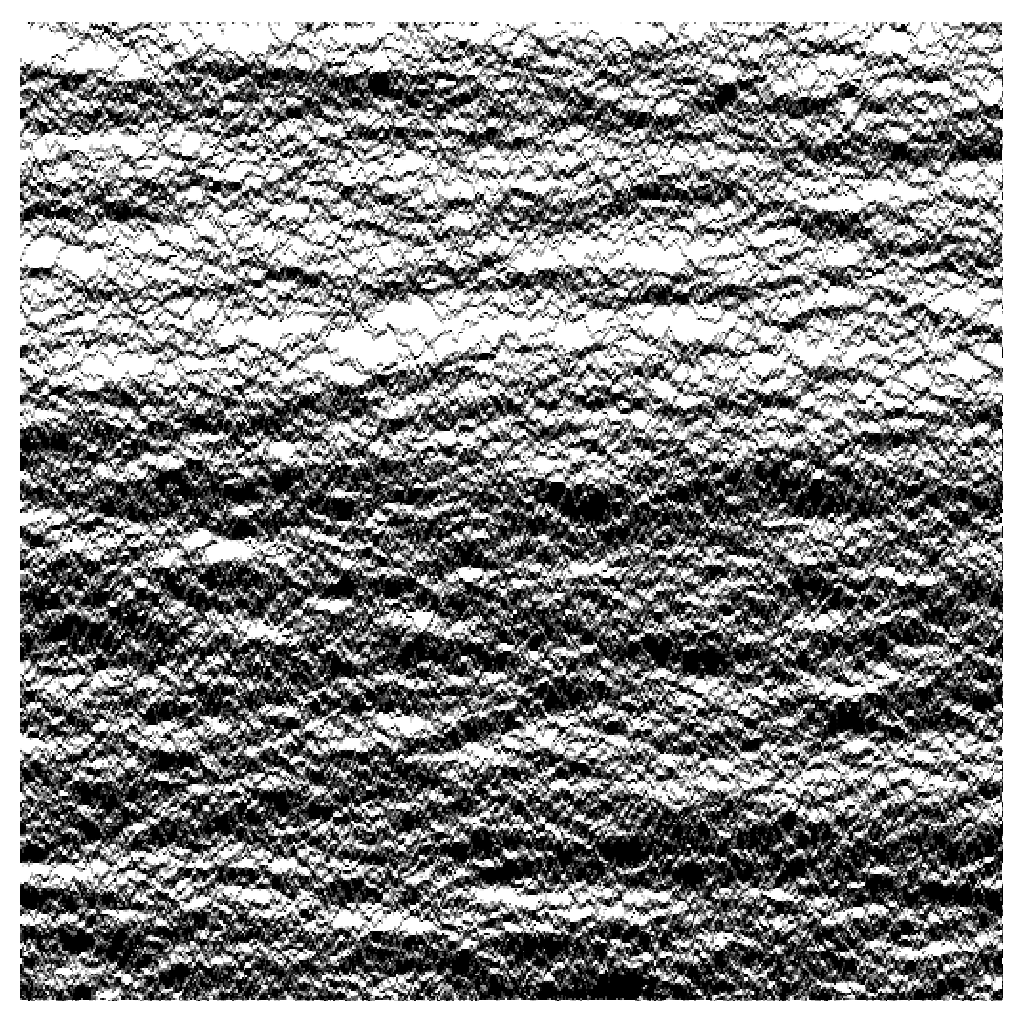
\includegraphics[width=0.31\linewidth]{numerics/images/stickyParticleFlows/flowImpL0p35T1p0.png} \\
\raisebox{5em}{256} & & 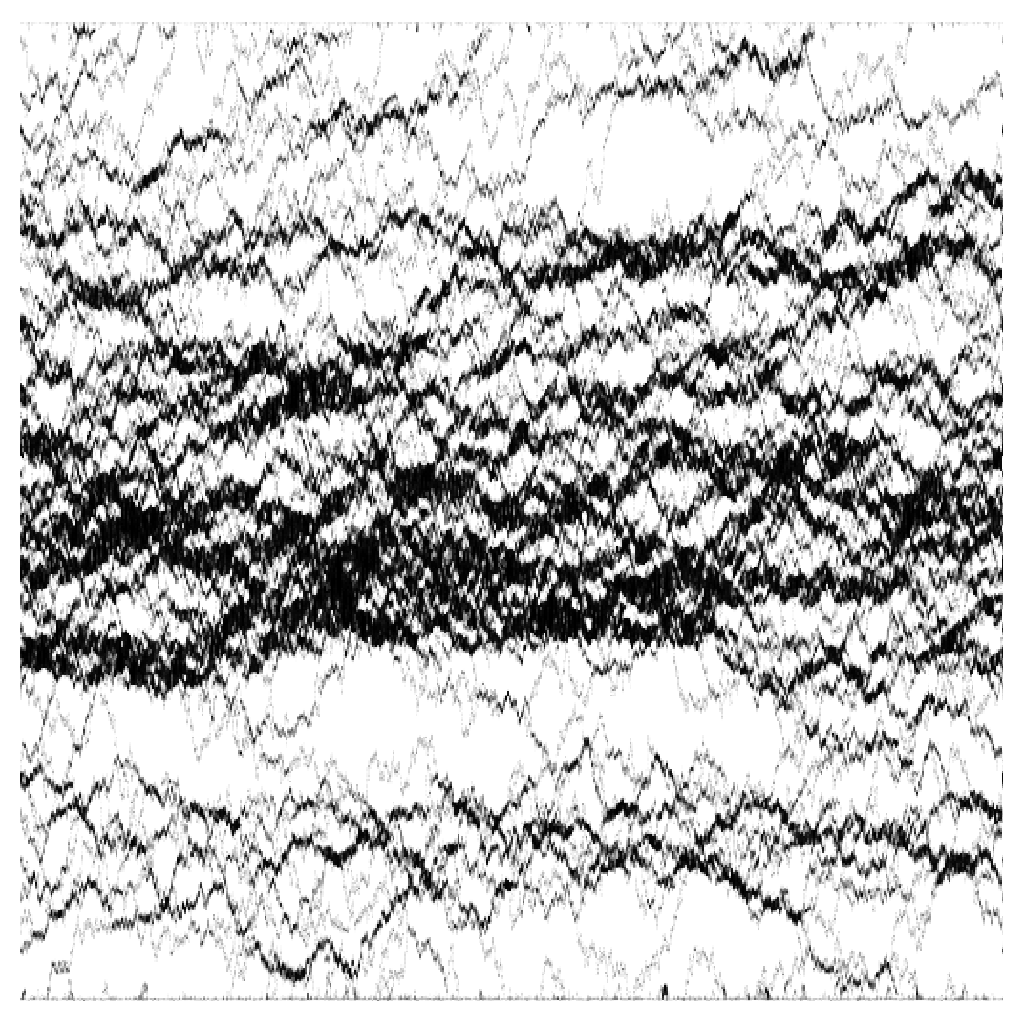
\includegraphics[width=0.31\linewidth]{numerics/images/stickyParticleFlows/flowImpL0p05T8p0.png} 
 & 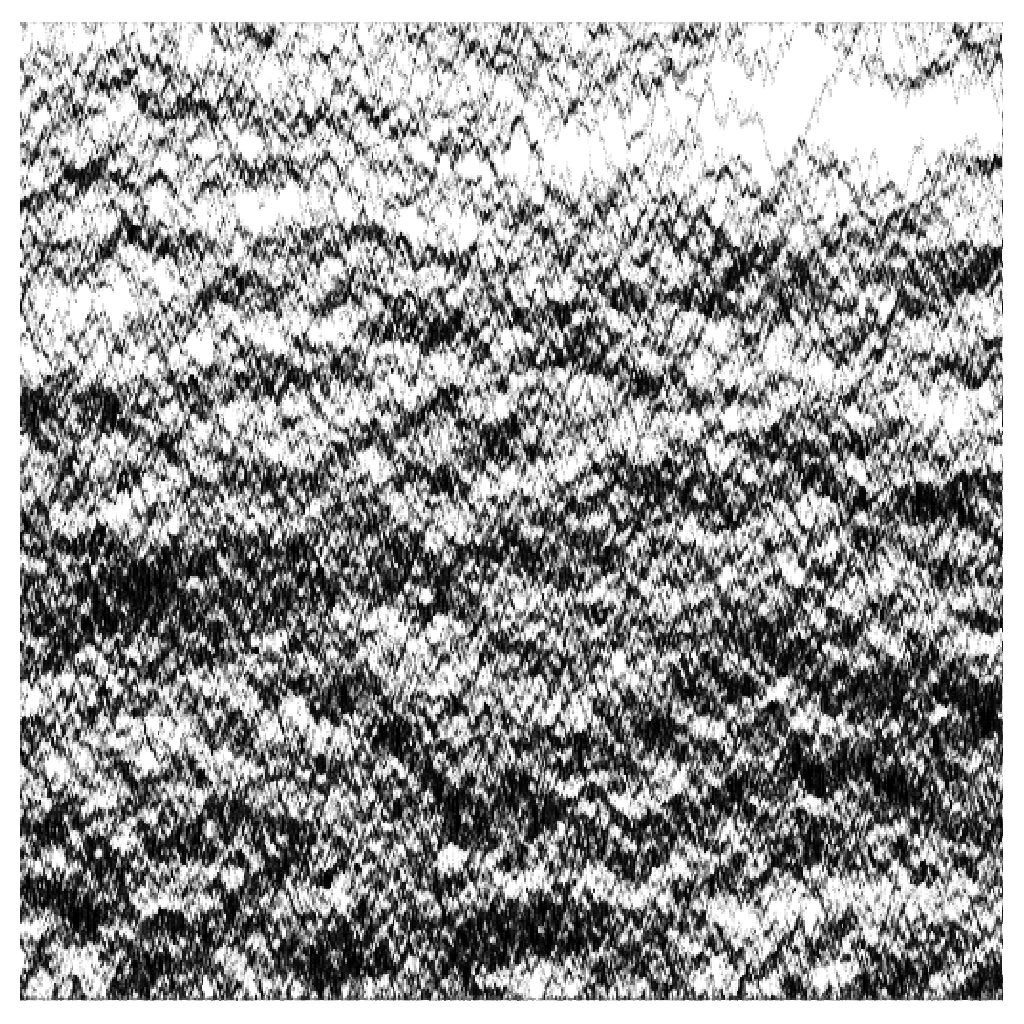
\includegraphics[width=0.31\linewidth]{numerics/images/stickyParticleFlows/flowImpL0p15T8p0.png} 
 & 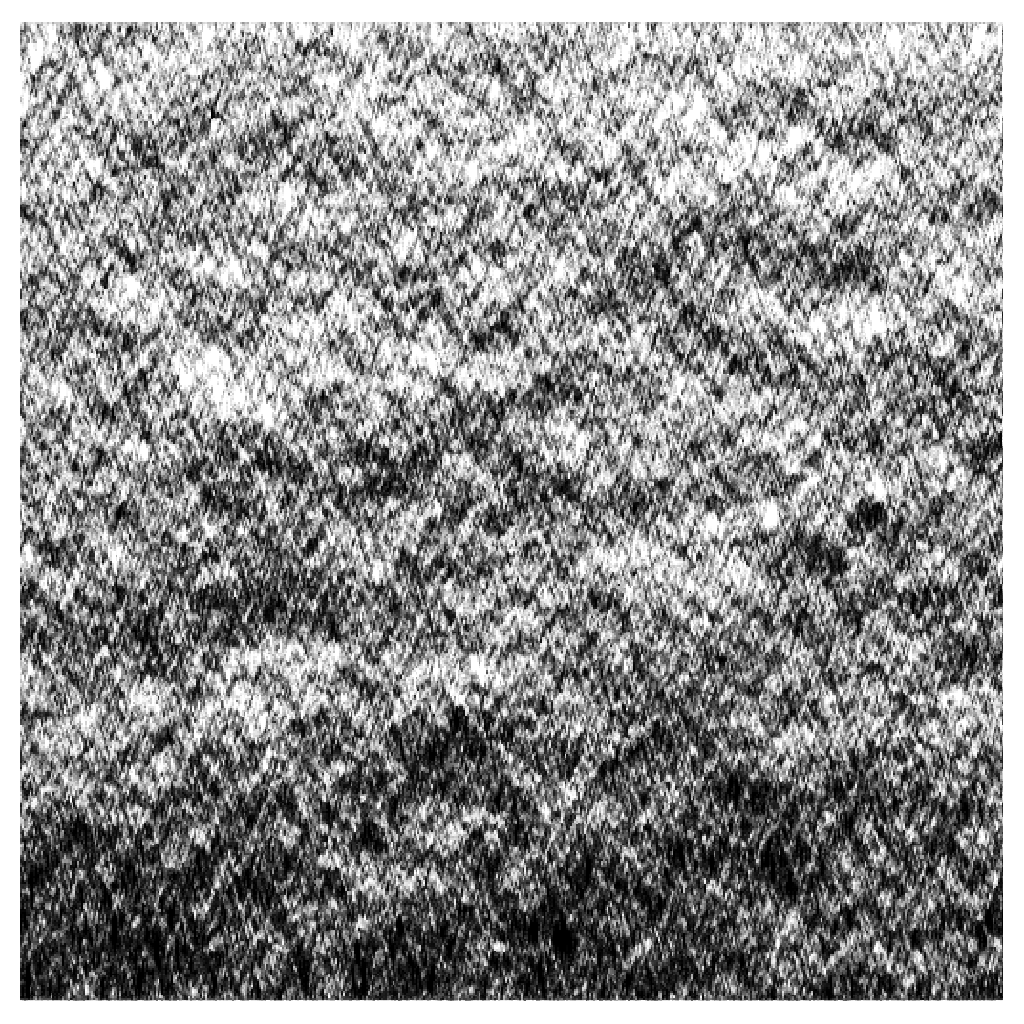
\includegraphics[width=0.31\linewidth]{numerics/images/stickyParticleFlows/flowImpL0p35T8p0.png} \\ 
\raisebox{5em}{1024} & & 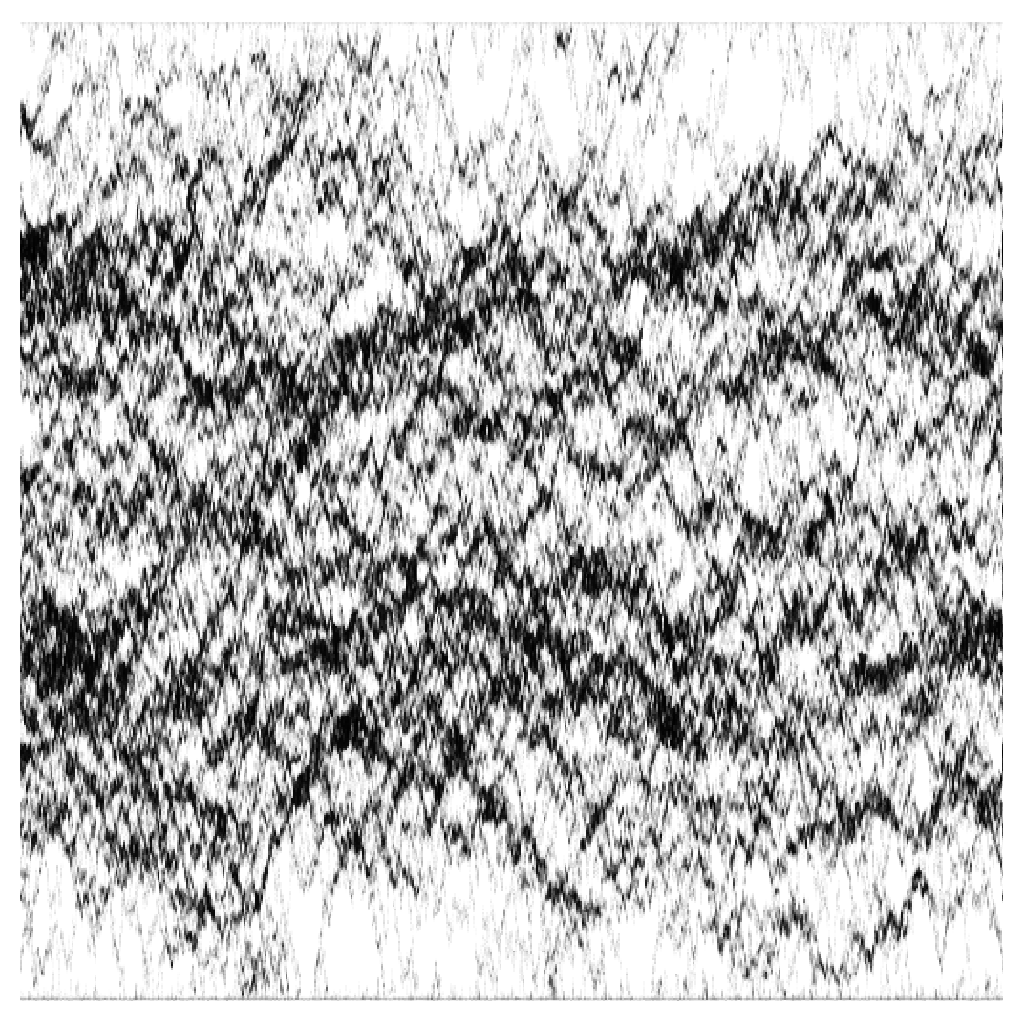
\includegraphics[width=0.31\linewidth]{numerics/images/stickyParticleFlows/flowImpL0p05T32p0.png} 
 & 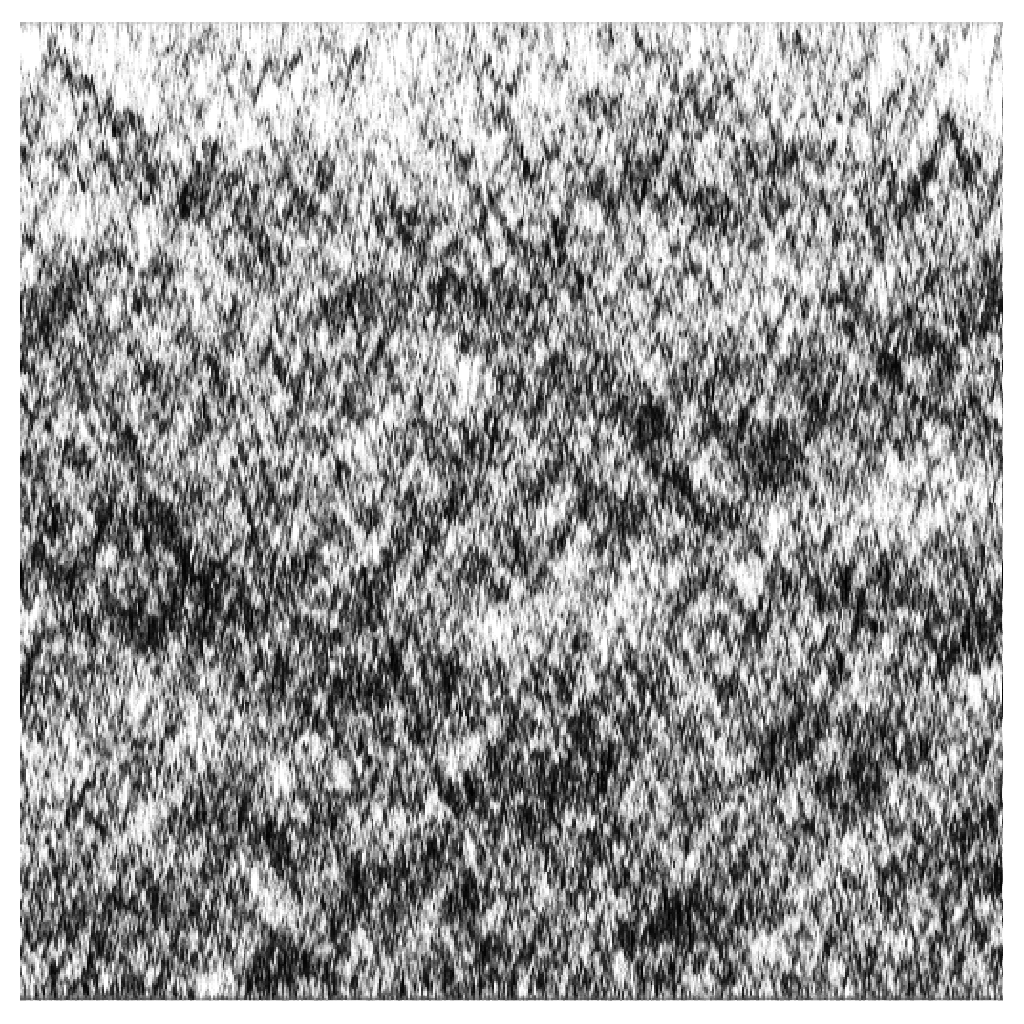
\includegraphics[width=0.31\linewidth]{numerics/images/stickyParticleFlows/flowImpL0p15T32p0.png}
 & 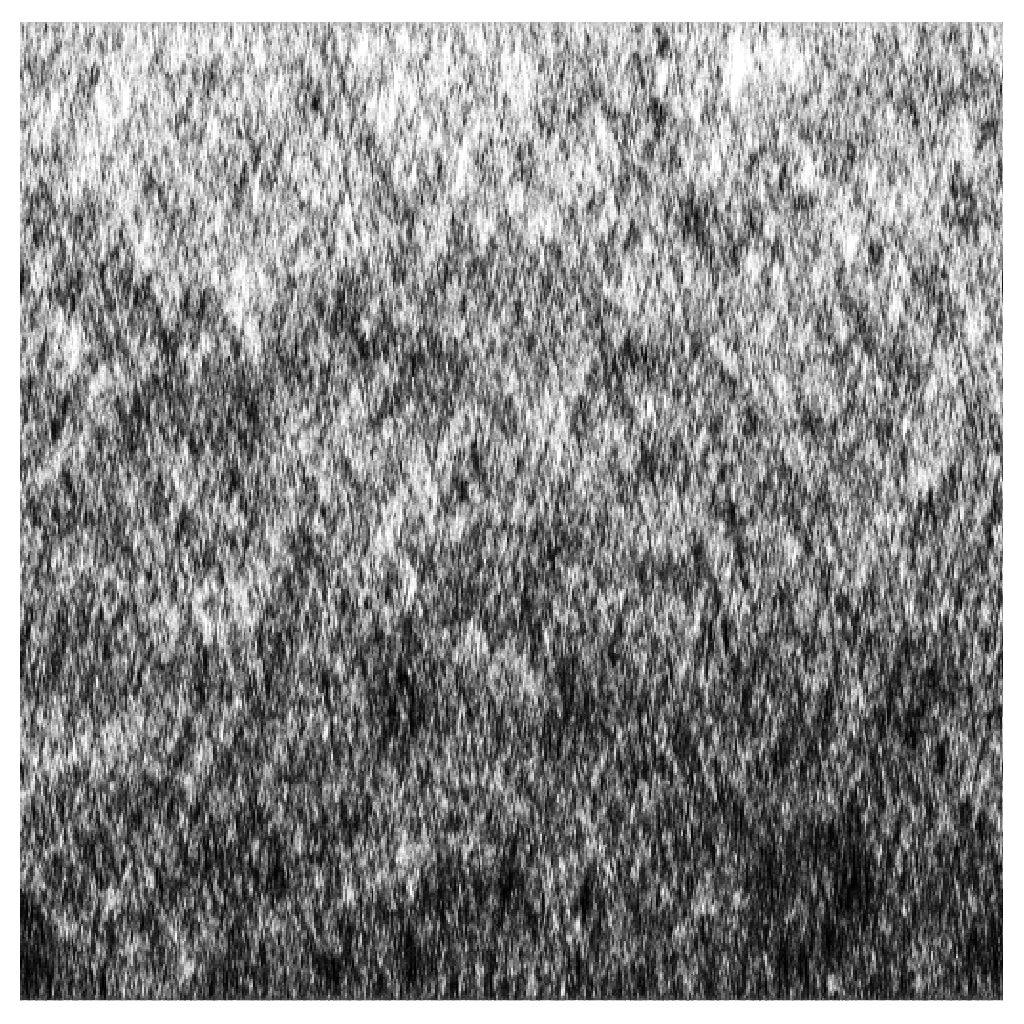
\includegraphics[width=0.31\linewidth]{numerics/images/stickyParticleFlows/flowImpL0p35T32p0.png} \\ 
\end{tabular}
\end{center}
 \end{figure}
 
Each of the systems here show the behaviour of particles with low-$\lambda$, so we are in the sticky regime;
however, all of our previous results indicate that there should be rather large differences in behaviour
as we switch from relatively weak stickiness (here embodied by $\lambda=0.35$) to strong stickiness
(portrayed by the $\lambda = 0.05$ situation). The images used to create Fig~\ref{fig:1DStickyPlots} are
relatively high-definition, which should enable readers using the digital copy to zoom in order to see the fine 
details. Our principle observations are as follows:
\begin{itemize}
 \item At the shortest timescale, one can quite clearly see the motions of individual particles. As one
 might expect, they are less likely to be seen unbound from neighbours in the lower-$\lambda$ systems than
 the higher-$\lambda$ ones. In the low-$\lambda$ regime, we are much more like to see big blocks of 
 particles, possibly containing a low concentration of mobile vacancies. Between these blocks we have a dilute
 ``gas'' of usually individual particles.
 \item Focussing now on the $32\times$ longer intermediate timeframe, we can see that in the extremely 
 low-$\lambda$
 situation we have blocks of particles separated by voids of vacancies. These voids contain a dilute gas
 of particles. Over these longer timescales, we see that the blocks of particles do in fact slowly migrate
 around the system, occasionally breaking apart or reforming during their travels. Also notice that the 
 voids are more likely to be found towards the centre of the system than adjacent to the boundaries.
 The chemical potential
 (Fig~\ref{fig:spmChemPot}) for small-$\lambda$ is minimised for high density, thus a boundary held at any
 density should be expected to in practise generate a high local density regardless of the density it is
 set to emulate; as we move away from the boundary its correlations with the interior weaken, so we think
 that the accumulation of particles on the boundary is an edge effect with a certain depth, and that the
 situation towards the centre of the system is more representative of the preferred bulk behaviour.
 \item Meanwhile for higher-$\lambda$, we see a ``tissue paper'' pattern over these intermediate
 timescales; the system is similar to a gas of randomly-walking particles, but there is a little bit more
 short-range correlation than that, hence the observed texture in the image.
 \item Now looking over longer timescales, we see that for the lowest-$\lambda$ it is in fact the case that 
 the voids towards the centre of the system do in fact appear and disappear over time. Given that we know 
 that there are still (small) flows occurring in this regime (see Sec~\ref{sec:lambdaScans}), it is
 likely that when these voids are created and destroyed, there are small overall biases in terms of
 which void boundaries more particles are extracted from or shed into. We suspect that
 this is the primary mechanism by which transport across the system is achieved in this regime. Meanwhile,
 the higher-$\lambda$ systems are becoming something closer to a continuous grey gradient from the top
 boundary to the bottom, suggesting that the overall transport is more diffusive in nature.
\end{itemize}



\subsubsection{Repulsive Particles}
Of course, we can do similar calculations with repulsive particles, for which $\lambda > 1$. Of the most
interest is the extreme case in which $\lambda >> 1$, when we should expect that particles have an almost 
explosive tendency to separate if brought together. We have performed such a calculation, with results
displayed in Fig~\ref{fig:1DRepulsePlots}, with a system
of length $L=1024$, $\lambda = 10^6$ and $(\rho_0 , \rho_L) = (0.99, 0.01)$, for which we performed $40960$
KMC steps. The time slices used in the plot are of size  $2 \times 10^{-7} \mathrm{s}$.
\begin{figure} \caption[The flow pattern of repulsive particles in $1$D]{Spacetime plot for a system of 
repulsive particles.} 
\label{fig:1DRepulsePlots}
\begin{center}
\begin{tabular}{c} 
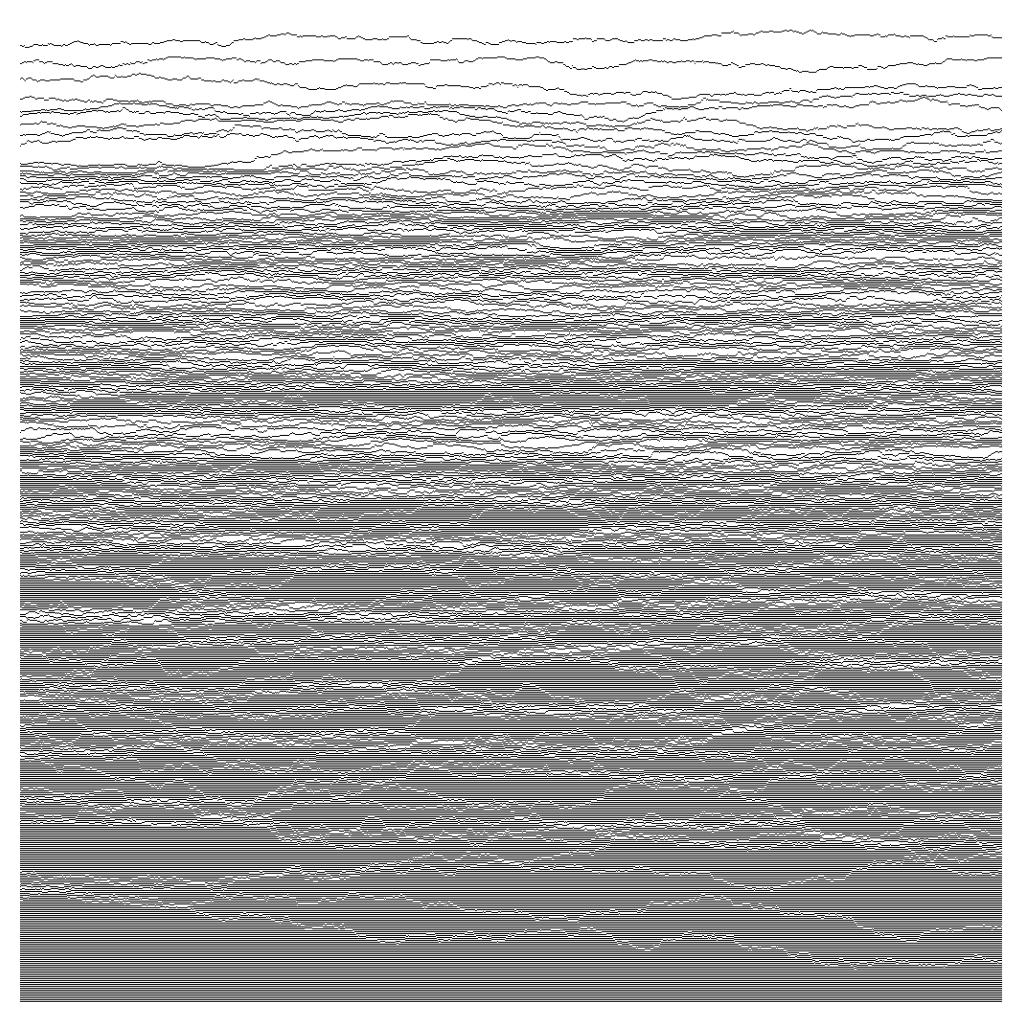
\includegraphics[width=0.8\linewidth]{numerics/images/stickyParticleFlows/aprilFlowStraight.png} \\
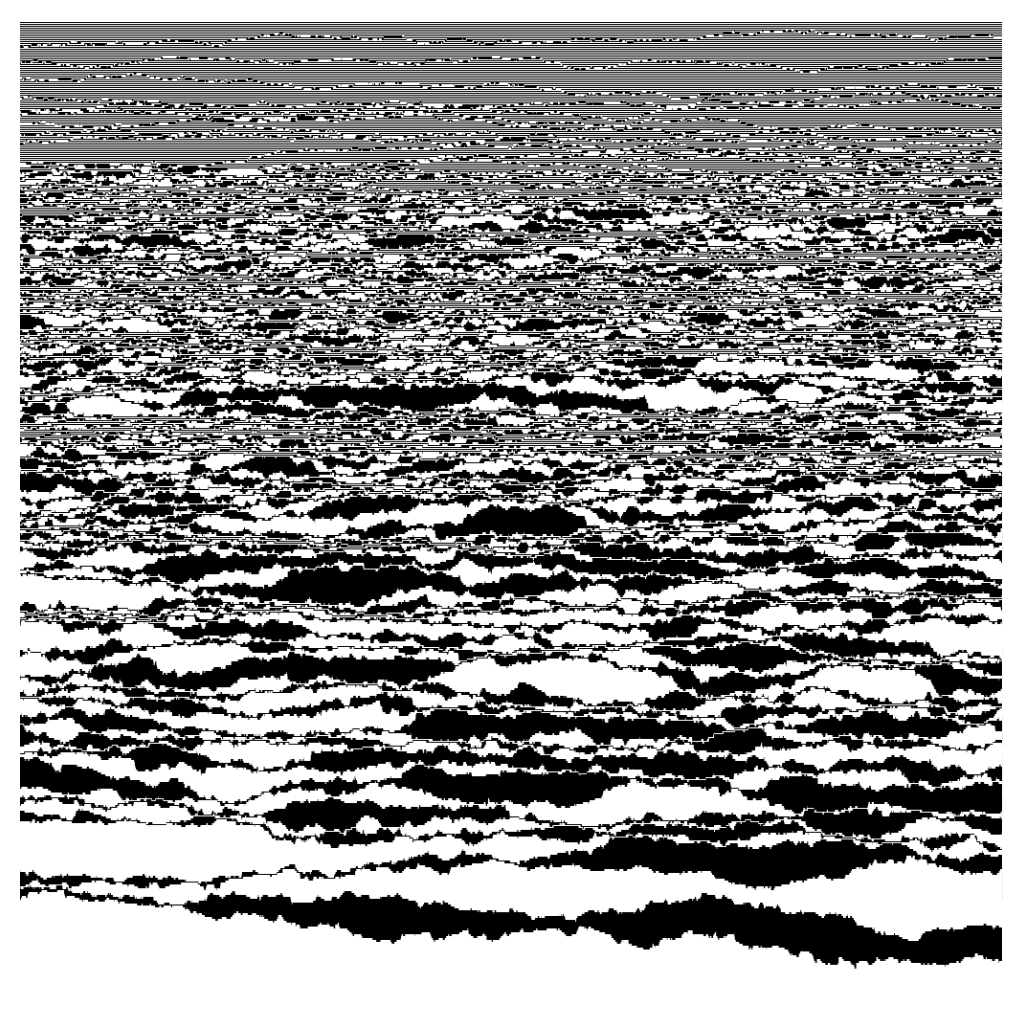
\includegraphics[width=0.8\linewidth]{numerics/images/stickyParticleFlows/aprilFlowDomains.png} \\
\end{tabular}
\end{center}
 \end{figure}
 
As before, time goes from left to right, space from top to bottom. 
The top plot displays the time-averaged density shaded the normal way (light being dense, dark being empty).
The bottom plot displays the same information, only this time we have applied the function $f(x) = 1-x$
to the density at every other site as we move along the spatial axis; thus we reveal that in this limit
our system is partitioned into domains, in the same way that an antiferromagnet might be. The boundaries
between these domains can move quite rapidly, and the motion of such a domain wall corresponds to the
transport of a particle; thus we think that it is this domain boundary motion which controls the rate
of transport in this regime.
 
 
\subsection{Scans Through $\lambda$ with Constant Boundary Densities} \label{sec:lambdaScans}
We can perform calculations in which we hold all things constant except $\lambda$, analogous to our 
existing calculations done using our TRM and MFT results. In these calculations, we computed the properties of systems with boundary densities $(\rho_0 , \rho_L )=(0.3, 0.1)$, $(0.75, 0.25)$ and 
$(0.9, 0.7)$, using both the evenly-timestepped Monte Carlo method and KMC. In this case, our KMC calculations used systems of size $L = 64$, whilst our other method used systems of size $L=100$.
To account for the different system sizes used, we have rescaled the current and its moments, whilst
leaving most other quantities such as particle density as they are. In the case of current, we have
multiplied by $L$ in order to achieve this normalisation; this is because a normal diffusive current is
driven by concentration gradient, therefore if we use the same concentration difference we should expect 
the resulting current to vary as $J \sim L^{-1}$. Note that for our KMC calculations we performed initial
equilibration runs of $4000000$ steps, followed by $1000$ of our alternating analysis/relaxation passes
of $16000$ steps each way; thus, this should provide us with decent quality data, at least until $\lambda$
becomes so small that particles can barely move through the system. Our evenly-timestepped calculations
were performed with $10000$ equilibration steps followed by a single measurement run of $100000000$ steps,
so we aren't calculating the other moments of the current using that method.

\subsubsection{Mean Current}
\begin{figure} \caption[The current flowing through systems as we vary $\lambda$ with constant boundaries,
$1$D]{The mean current observed to flow from a boundary with greater particle density to lesser particle 
density in $1$D. Here the boundary densities are held constant throughout, whilst $\lambda$ is varied.
The lower plot is the same data as the upper one, but with logarithmic axes instead of linear ones.
The dashed lines
correspond to the MFT predictions, the joined circles to TRM-computed results, the triangles to results
computed using evenly-timestepped Monte Carlo and the crosses to KMC calculations.} 
\label{fig:1DlambdaScans}
\begin{center}
\begin{tabular}{c} 
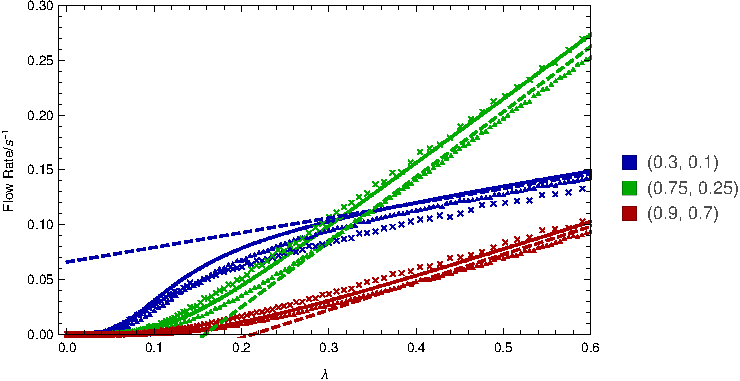
\includegraphics[width=1.1\linewidth]{numerics/images/lambdaScan/allDataLinear} \\
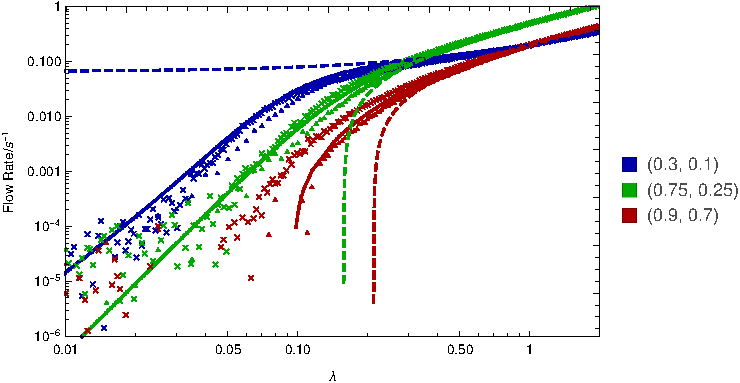
\includegraphics[width=1.1\linewidth]{numerics/images/lambdaScan/allData} \\
\end{tabular}
\end{center}
\end{figure}

Fig.~\ref{fig:1DlambdaScans} displays the variation of the current with $\lambda$. Here, the dashed lines
correspond to the MFT predictions, the joined circles to TRM-computed results, the triangles to results
computed using evenly-timestepped Monte Carlo and the crosses to KMC calculations.
Fig.~\ref{fig:1DlambdaScansLogged} displays the same data, but over a wider range of $\lambda$ values.
We have already discussed the TRM results and their relation to the MFT results back in 
Sec.~\ref{sec:TRMLambdaScan}. Our main observations about the current are as follows:
\begin{itemize}
 \item At large $\lambda$ the current seems to vary in proportion to $\lambda$, in agreement with our
 TRM and MFT results. The actual constants of proportionality don't quite match, which is a common issue
 in all of these results. We have seen in Sec.~\ref{sec:flowPatternVis} that there is usually a boundary
 layer of excess particles or vacancies next to both boundaries, thus it is possible that this issue
 arises from this boundary layer causing the current to not scale with $L$ in quite the way we
 expect. However, this is something we can check by varying the system size and checking the current
 variation with $\lambda$, as we have done in Fig.\ref{fig:lambdaScanRepeats}.
 \item For $\lambda \in (0.01, 0.3)$, the current undergoes power law variation with $\lambda$, again in 
 agreement with our TRM calculations, with $J \propto \lambda^{3}$.
 \item For smaller values of $\lambda$, the observed mean current starts to become noisy, at least in the
 logarithmic plots, and essentially saturates to a low value. Our interpretation of this is that for these
 extreme low values of $\lambda$ the current signal becomes extremely weak, as it begins to depend on the
 motions of extremely small overall numbers of particles during the measurement period; thus, in that 
 regime the current is dominated by a form of shot noise, and so it becomes difficult to measure the current accurately in this regime.
\end{itemize}

\begin{figure} \caption[As Fig.~\ref{fig:1DlambdaScans} but over a much wider range of $\lambda$-values.]{As the logarithmic plot in Fig.~\ref{fig:1DlambdaScans} but over a  much wider range of $\lambda$-values.} 
\label{fig:1DlambdaScansLogged}
\begin{center}
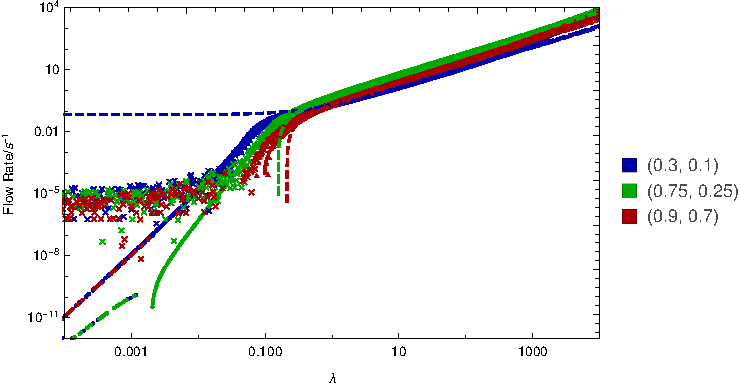
\includegraphics[width=1.0\textheight, angle=270]{numerics/images/lambdaScan/allDataWide}
\end{center}
\end{figure}

Thus, we still seem to see the same ``transition'' we saw when analysing TRM results. To ensure that this
behaviour in the current isn't just an artefact of system size, we can vary the system size whilst
measuring the current, as we have done in Fig.~\ref{fig:lambdaScanRepeats}.
\begin{figure} \caption[Calculations of the dependence of current upon $\lambda$, repeated with different system sizes.]{Calculations of the dependence of current upon $\lambda$, repeated with different system sizes as indicated. Here we have focussed on the boundary setup 
$(\rho_0, \rho_L) = (0.75, 0.25)$ and region $\lambda \in (0.04, 0.25)$, which constitutes the
bend in our supposed transition. Standard errors in the current were computed using observed current 
variances.} 
\label{fig:lambdaScanRepeats}
\begin{center}
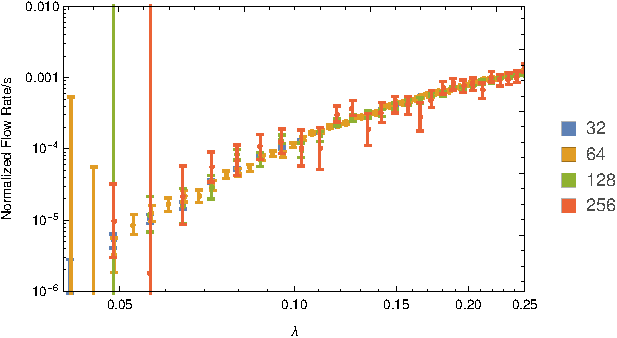
\includegraphics[width=0.95\textheight, angle=270]{numerics/images/lambdaScan/lambdaScanRepeatFlows}
\end{center}
\end{figure}

Here we see that our method for normalising currents for different system sizes actually seems
to work quite well, at least over the system sizes we are looking at. It also indicates that our choice of
$L=64$ behaves well until $\lambda < 0.05$, at which point the fluctuations start to become very large 
compared to the observed mean current.

\subsubsection{Current Higher Moments}
Using our KMC calculations, we can also compute the higher moments of the current. As we do not have any 
particular theory which predicts these higher moments, we do not have very much to say about these
results, other than simply stating what we see. It is worth noting that we don't detect divergences
in these moments around the bend of our ``transition'', therefore it does not seem to be a transition
in the traditional phase transition sense, as there we would expect to see discontinuities in observables,
and here current is the kind of observable we should expect to manifest that kind of behaviour.
These moments, up to and including the current kurtosis, are displayed in 
Fig.~\ref{fig:lambdaScanHigherMoments}. Note that no units for skewness and kurtosis are listed
as they have already been normalised using the scale set by the variance.
\afterpage{
\begin{figure} \caption[Higher moments of the current, in 1$D$]{The higher moments of the current, 
measured in the same setup as used in Fig.~\ref{fig:1DlambdaScans}.} 
\label{fig:lambdaScanHigherMoments}
\begin{center}
\begin{tabular}{c} 
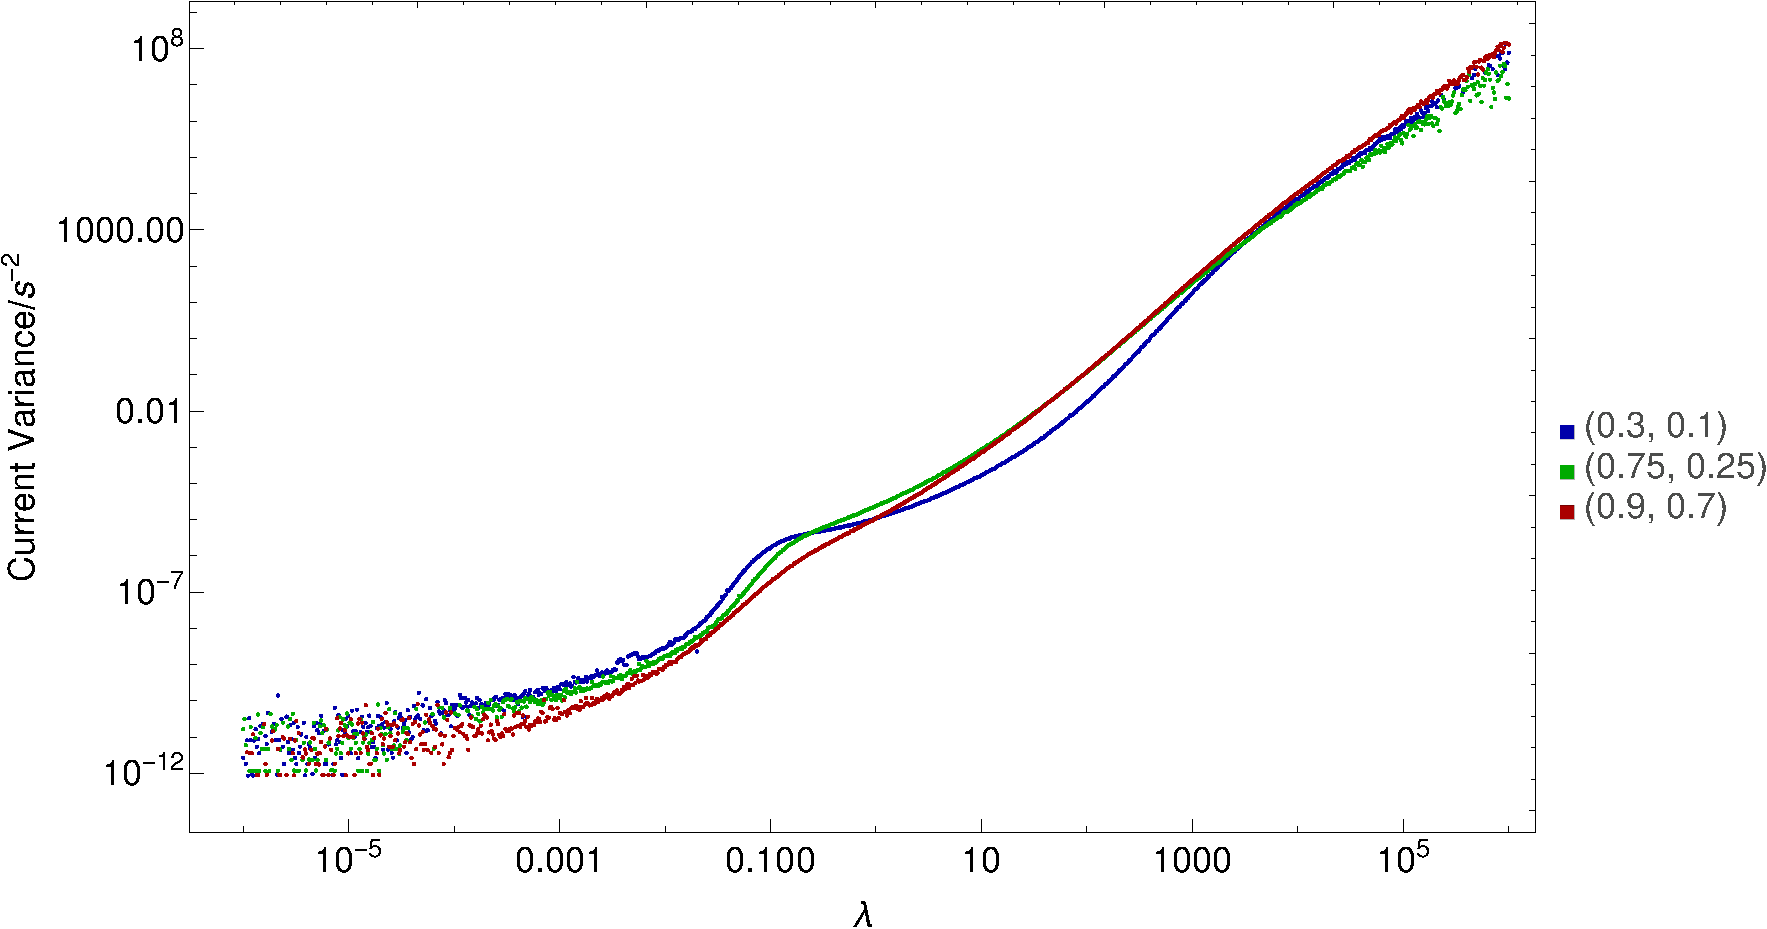
\includegraphics[width=1.0\linewidth]{numerics/images/lambdaScan/lambdaScanVar} \\
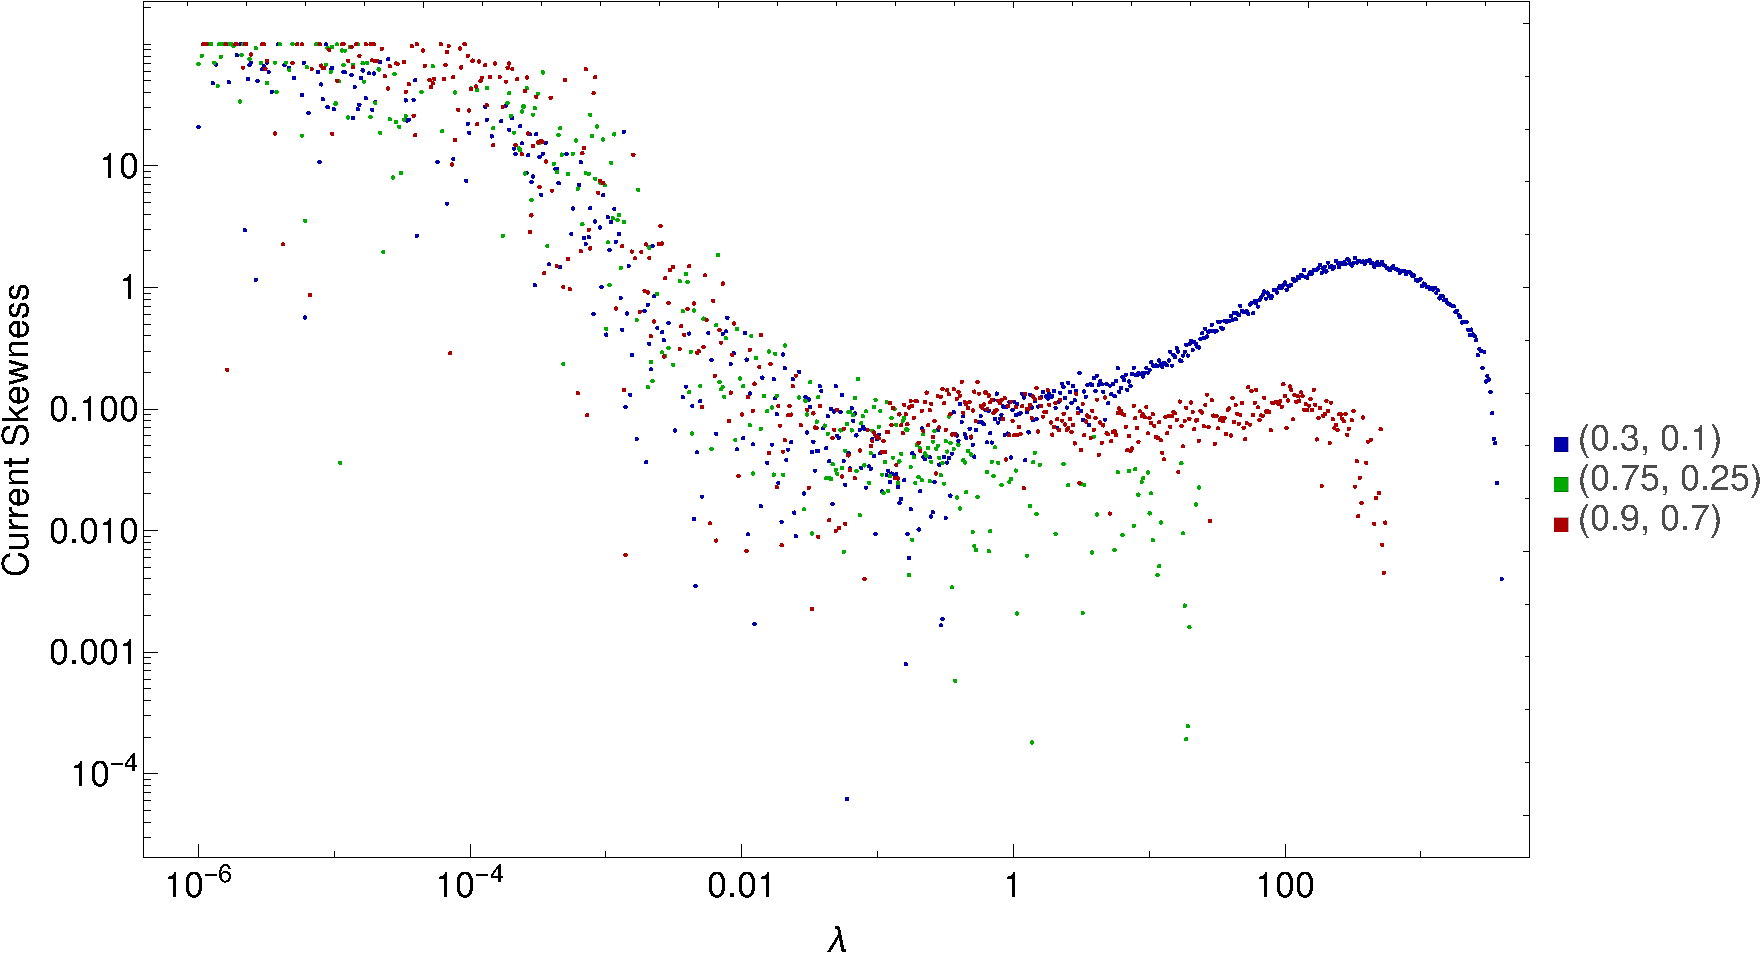
\includegraphics[width=1.0\linewidth]{numerics/images/lambdaScan/lambdaScanSkew} \\
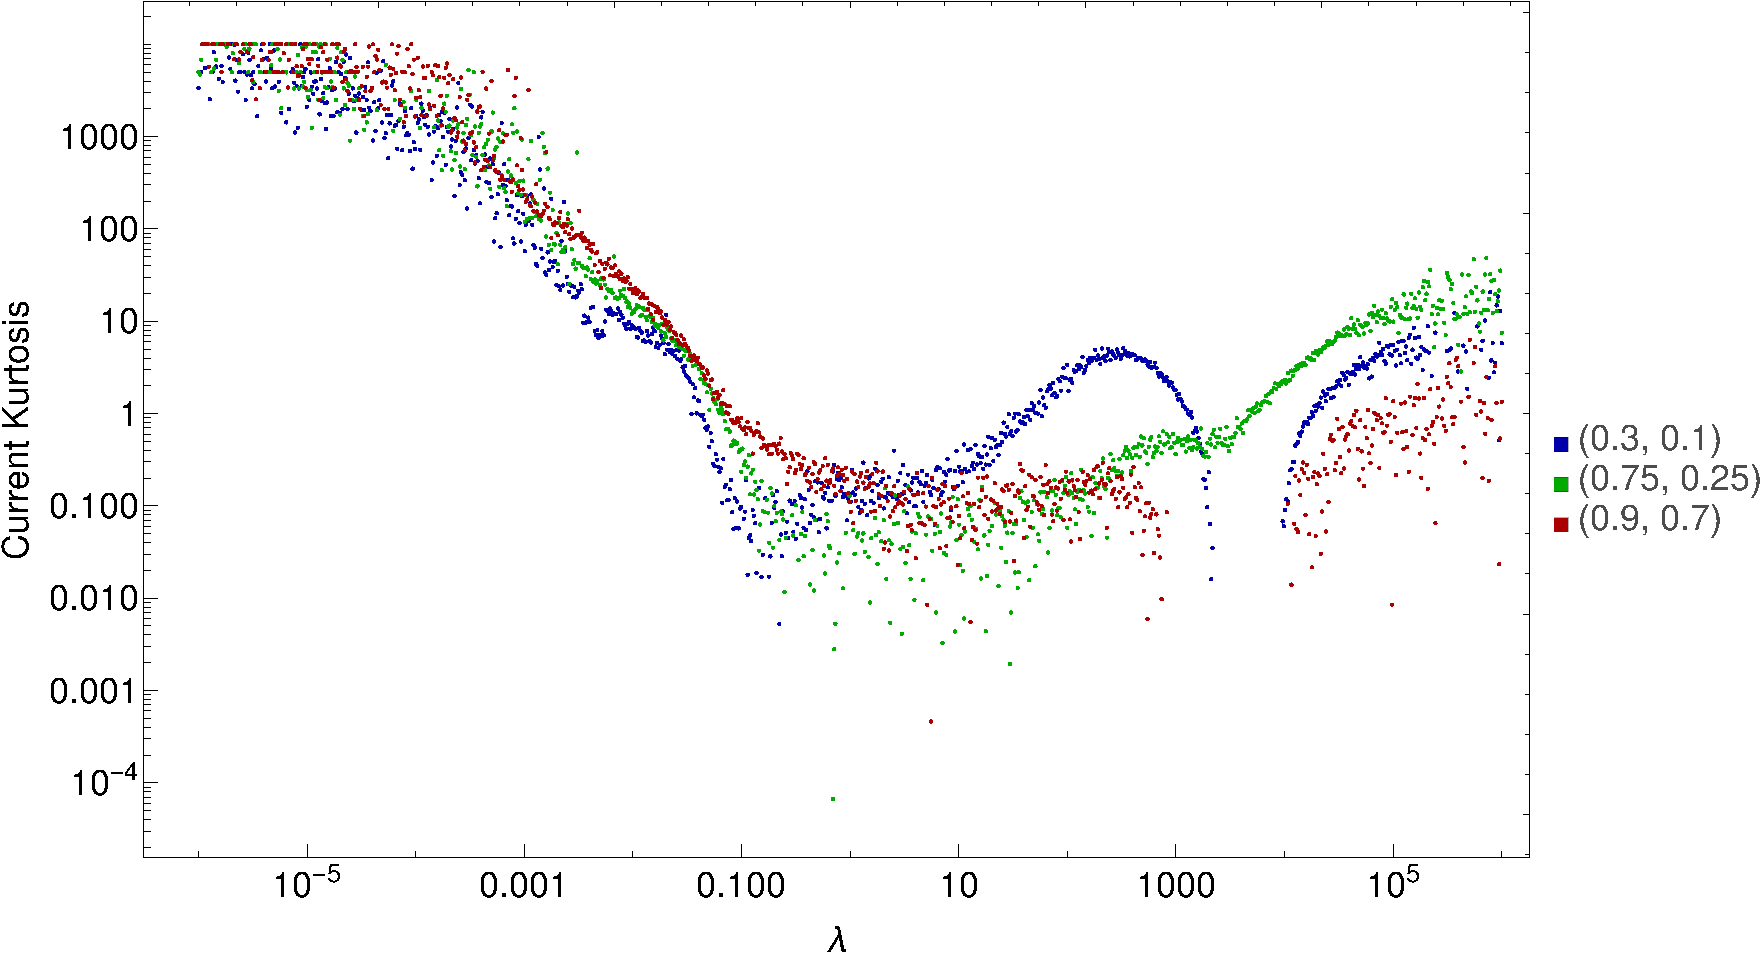
\includegraphics[width=1.0\linewidth]{numerics/images/lambdaScan/lambdaScanKurt} \\
\end{tabular}
\end{center}
\end{figure}
\clearpage
}

There's a little bit of a bend in the variance as we go through the transition, but nothing major.
Skewness is typically positive but fluctuates a lot, and goes negative past certain thresholds at
large $\lambda$. Kurtosis is bounded and possibly negative for $\lambda$ above the transition threshold,
then starts growing large and positive as we go through the suspected transition.
Thus, we have several different pieces of weak evidence of something happening in the transition region,
but nothing clear and conclusive like a spike or discontinuity.


\subsubsection{Overall Density}

In addition to measuring current and its moments, we can measure the mean overall density of particles in
the system. We did this using the same system parameters as in Fig.~\ref{fig:1DlambdaScans}; the 
variation in this mean density with $\lambda$ for different boundary conditions is displayed in 
Fig.~\ref{fig:lambdaScanDensityMean}.
\afterpage{
\begin{figure} \caption[The variation of the overall mean density of the SPM system with $\lambda$ for different boundary conditions, in $1$D.]{The variation of the overall mean density of the SPM system with $\lambda$ for different boundary conditions, in $1$D. 
Setup is the same as in Fig.~\ref{fig:1DlambdaScans}.} 
\label{fig:lambdaScanDensityMean}
\begin{center}
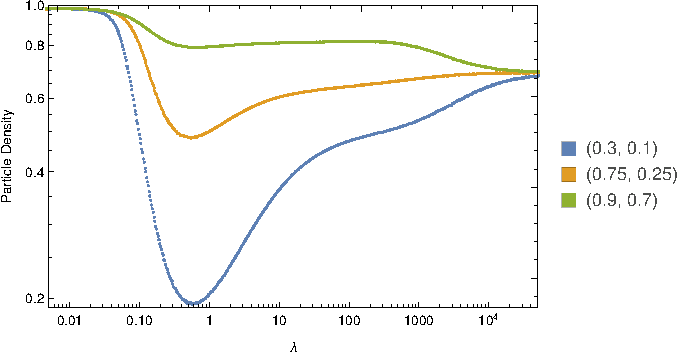
\includegraphics[width=0.95\textheight, angle=270]{numerics/images/lambdaScan/wideDensProfiles}
\end{center}
\end{figure}
\clearpage
}

The most striking feature here is how the densities converge for extreme values of $\lambda$
regardless of the actual boundary conditions used, converging to $1$ for extremely small $\lambda$ and to
around $\frac{2}{3}$ for extremely large $\lambda$. The behaviour seen here is in accordance with our 
existing computations as seen in \ref{sec:TRMDensityCurrent}, and our theory about this is as expressed 
there: in short, that at small $\lambda$, high density is favoured for ``energetic'' reasons (the
attempted minimisation of equilibrium  free energy), whilst at very large $\lambda$  our system self-
organises to have a density of $\sim \frac{2}{3}$ in order to enable maximal flow to occur due to a
stability argument.

We can also measure the variance of the densities we observed, and use this to gauge the size of the
density fluctuation, $\Var(\rho)$. In the results displayed in Fig.~\ref{fig:lambdaScanDensityFluc}, we have
computed the density fluctuation in our $1$D SPM system with boundary conditions
$(\rho_0, \rho_L) = (0.6, 0.4)$, using the evenly-timestepped Monte-Carlo method. Here we have
calculated this fluctuation for systems of various different sizes, and then normalised the fluctuation
via multiplication by system size. Note that we have two datasets for $L=400$ as we used two different
numbers of timesteps to see what impact it had.
\begin{figure} \caption[The variation of the fluctuation of the  density of the SPM system with 
$\lambda$ for different boundary conditions, in $1$D.]{The variation of the fluctuation of the density
observed in the SPM system with $\lambda$ for different boundary conditions, in $1$D.} 
\label{fig:lambdaScanDensityFluc}
\begin{center}
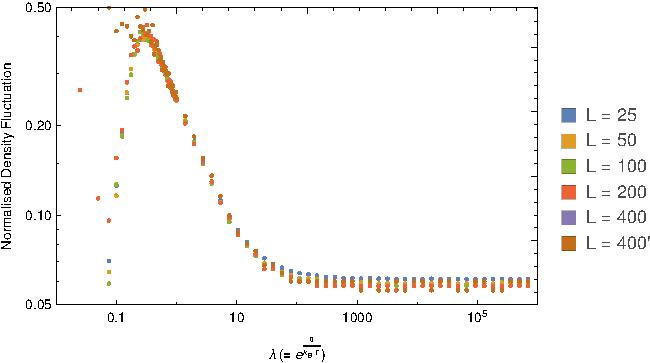
\includegraphics[width=0.95\textheight, angle=270]{numerics/images/lambdaScan/normDenFluc}
\end{center}
\end{figure}

As this causes the points to generally align for $\lambda>0.3$, this suggests that in that regime the 
dependence of $L \times \Var (\rho)$ upon $L$ is pretty weak; therefore,
the density fluctuation scales as $\mathcal{O}(L^{-1})$, implying that the number of particles in the
system fluctuates as $\mathcal{O}(1)$, which makes perfect sense when you consider that the system
allows particles to enter and leave the system only at the two boundaries, which do not change with the
system size in any sense. We also observe that there is a visible bump as we pass through the suspected
transition, but as with our higher current moments it is not a spike or discontinuity. We also
observe that for the smaller systems the fluctuation comes back under control as $\lambda$ keeps getting
smaller, whilst for larger ones the fluctuations remain large. We suggest that this is due to the fact
that we have observed the fluctuations over some timescale; thus if the system is undergoing long, slow
fluctuations over timescales longer than our observation frame, we will underestimate these fluctuations.
This is in essence a ``time to equilibration'' error, in the sense that the system's equilibration
timescale is longer than our observation timescale, and this informs us that we should be dubious about
our larger-$L$ results once we get into the extremely small $\lambda$ regime.

\subsubsection{Block Size Distribution}
The final type of measurement we have recorded in this ``$\lambda$-scan'' series of calculations is
the distribution of block sizes. By this we mean that we observe how many contiguous runs of $1$, $2$ 
and so on particles there are and add these to a time-weighted histogram, as per our method outlined in
Sec.~\ref{sec:kmcLib}. If we do this, again using our run parameters from
Fig.~\ref{fig:lambdaScanDensityFluc}, we find that the mean block size and its standard error vary
as shown in Fig.~\ref{fig:blockSizeDistn}.
\begin{figure} \caption[The mean block size and its standard error.]{The mean block size and associated
standard error, using the same run parameters as we did for Fig.~\ref{fig:1DlambdaScans}.} 
\label{fig:blockSizeDistn}
\begin{center}
\begin{tabular}{c} 
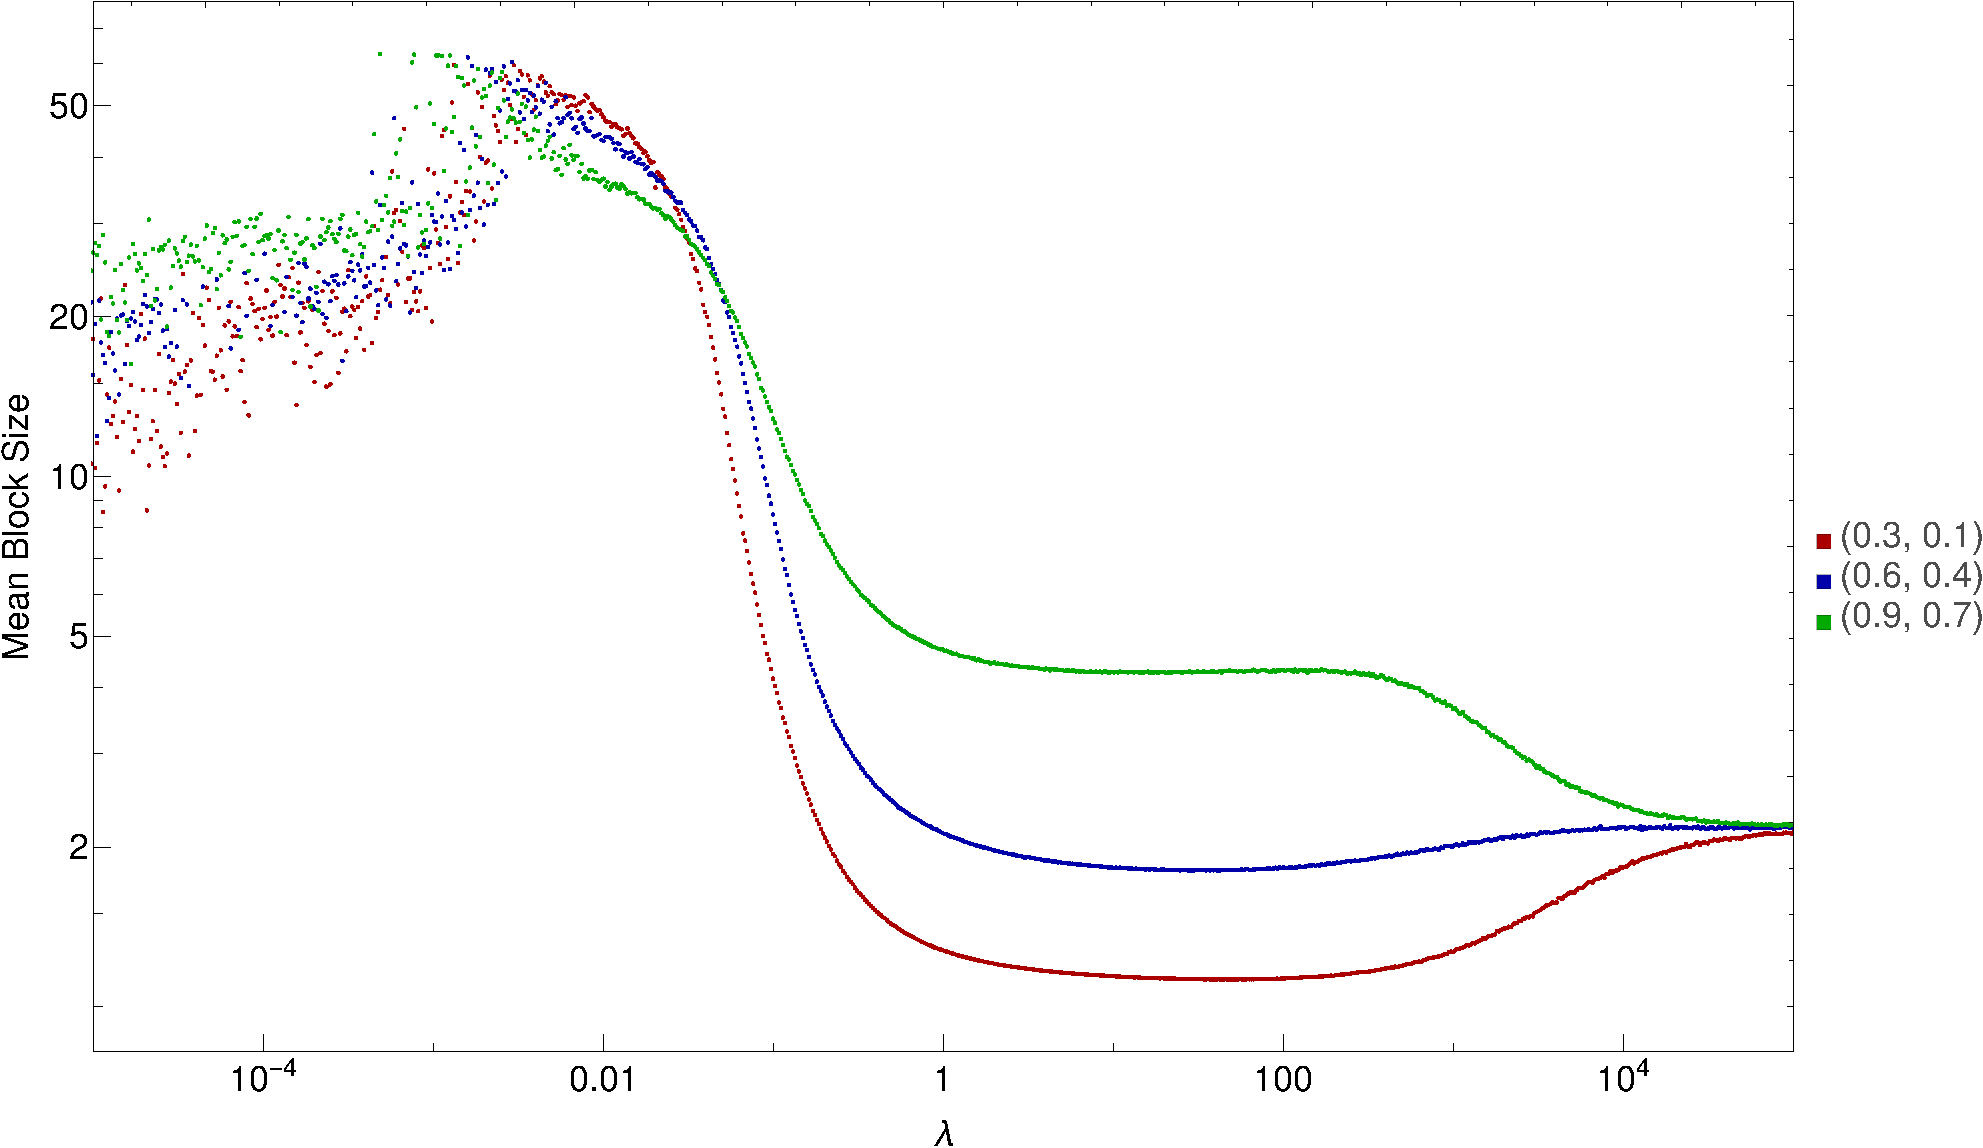
\includegraphics[width=1.0\linewidth]{numerics/images/lambdaScan/blockSizeMeans} \\
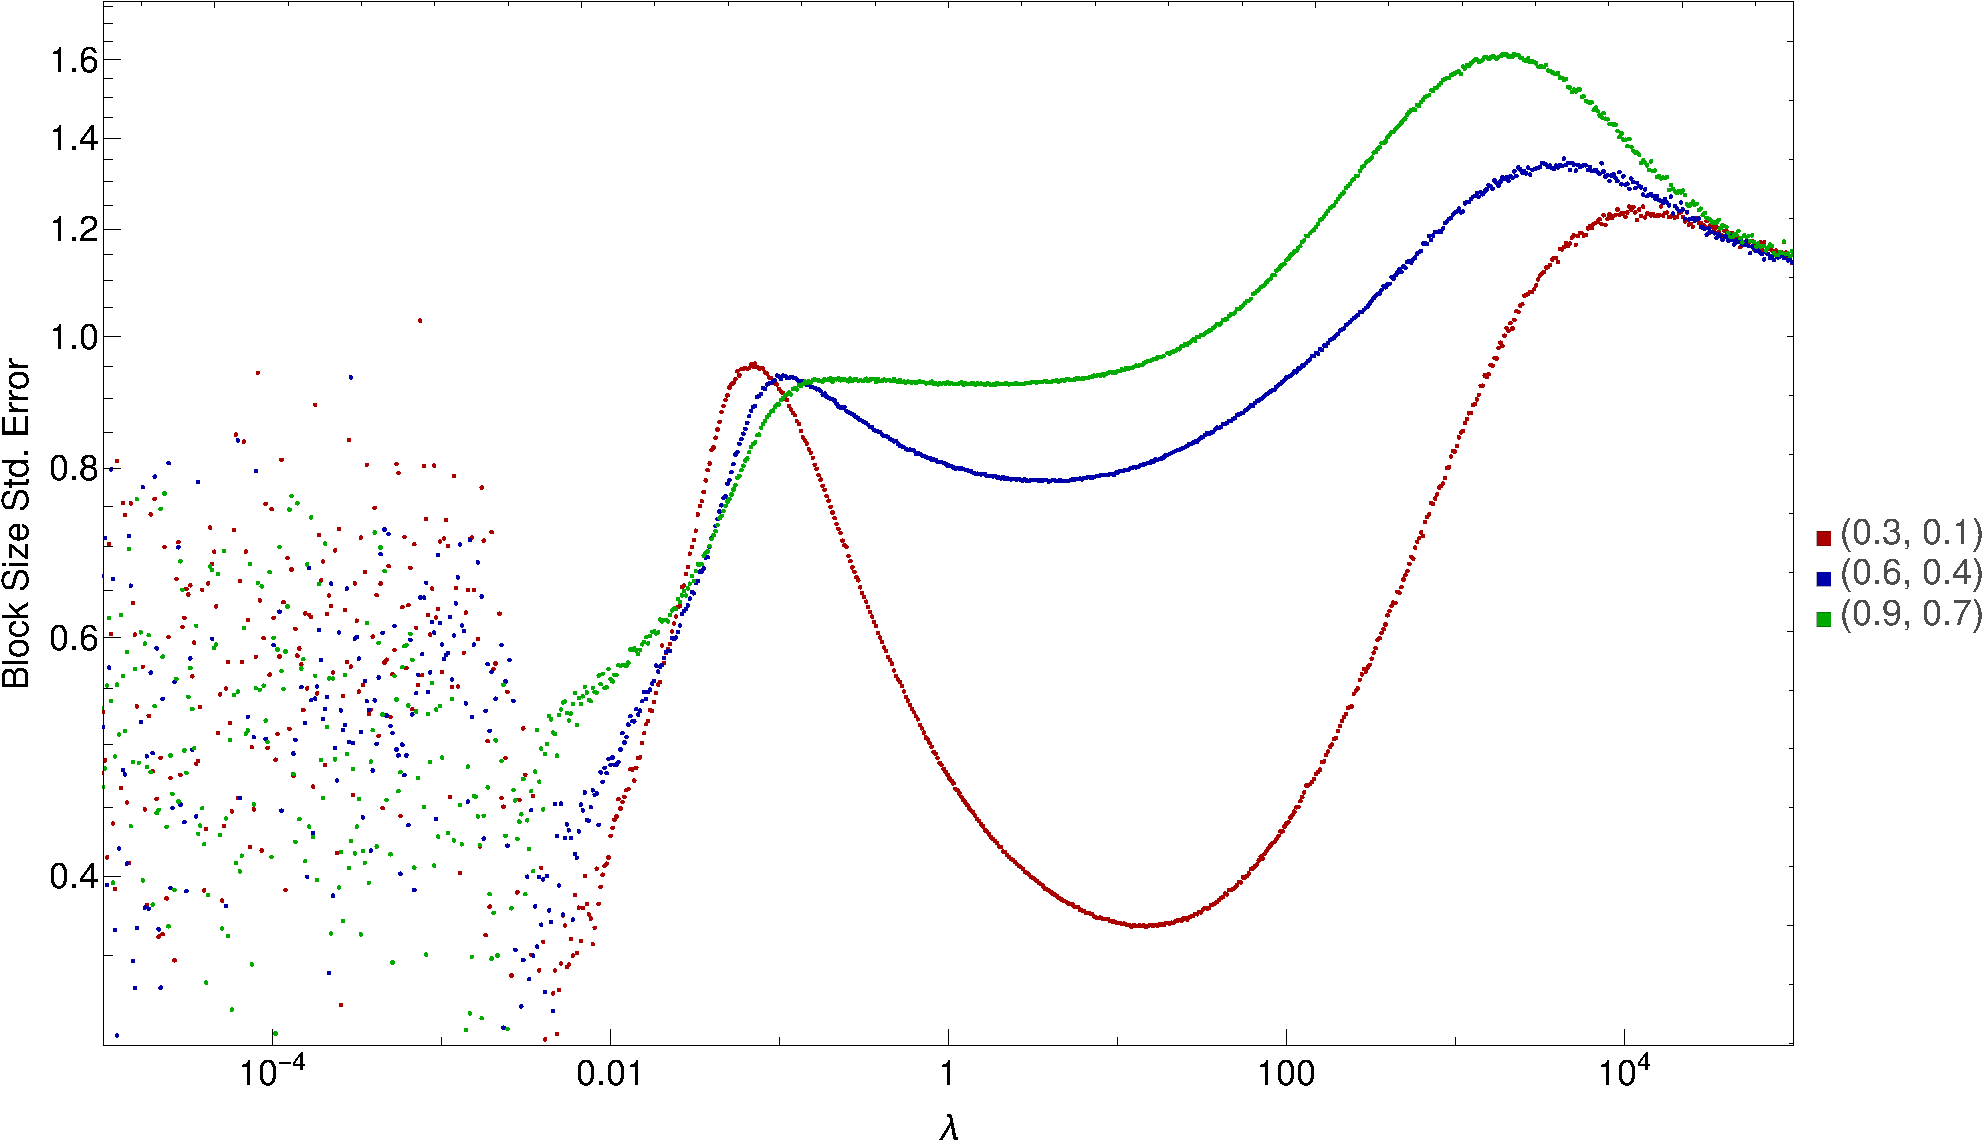
\includegraphics[width=1.0\linewidth]{numerics/images/lambdaScan/blockSizeStdErr} \\
\end{tabular}
\end{center}
\end{figure}

Here we once again see that we have convergence in the large-$\lambda$ limit, to an average block
size very close to $2$ which is in line with our ideas about maximal transport with a density of 
$\frac{2}{3}$. As we go towards $\lambda=1$, we find that the block size distribution reverts to
that which we'd expect by just randomly arranging particles with given densities, which is essentially
what is happening in SEP. As we go through the transition, the mean block size suddenly takes off,
whilst the fluctuation in the block size peaks, before once again starting to reduce. Once we get to 
very small $\lambda$, we lose the signal in noise, in a similar way to how we see all our results become
noise-dominated in the extremely small $\lambda$ regime.


\subsection{Varying $\lambda$ and Boundary Density Difference Together} \label{sec:constDens}
Another type of calculation we can perform is one in which we hold the average of the boundary 
densities constant, whilst varying their difference and $\lambda$; we can do this by using boundary
conditions $(\rho_0, \rho_L)=(\rho + \frac{1}{2} \delta \rho , \rho - \frac{1}{2} \delta \rho)$ and 
varying $\delta \rho$ whilst keeping $\rho$ constant. In our calculations
of this style, we set $\rho=\frac{1}{2}$, $L=64$, performed $400000$ 
equilibration steps and then $1000$ alternating measurement and relaxation
runs of $16000$ and $1000$ steps respectively. From this we calculated
the same kinds of quantities as in Sec.~\ref{sec:lambdaScans}; the 
principle results are displayed in Fig~\ref{fig:constDens}.
\begin{figure} \caption[Results obtained by fixing the average of the boundary densities and varying their difference and $\lambda$]{The main results. obtained by having boundary densities 
$(\rho_0, \rho_L)=(\rho + \frac{1}{2} \delta \rho , \rho - \frac{1}{2} \delta \rho)$. 
Here $\rho=\frac{1}{2}$. Clockwise from top left, we have: The mean current, the current variance,
the mean block size, and the mean overall system density. Note that in our mean block size
computation, many calculations failed; this explains the sparsity of the data in the right
of the image.} 
\label{fig:constDens}
\begin{center}
\begin{tabular}{c c} 
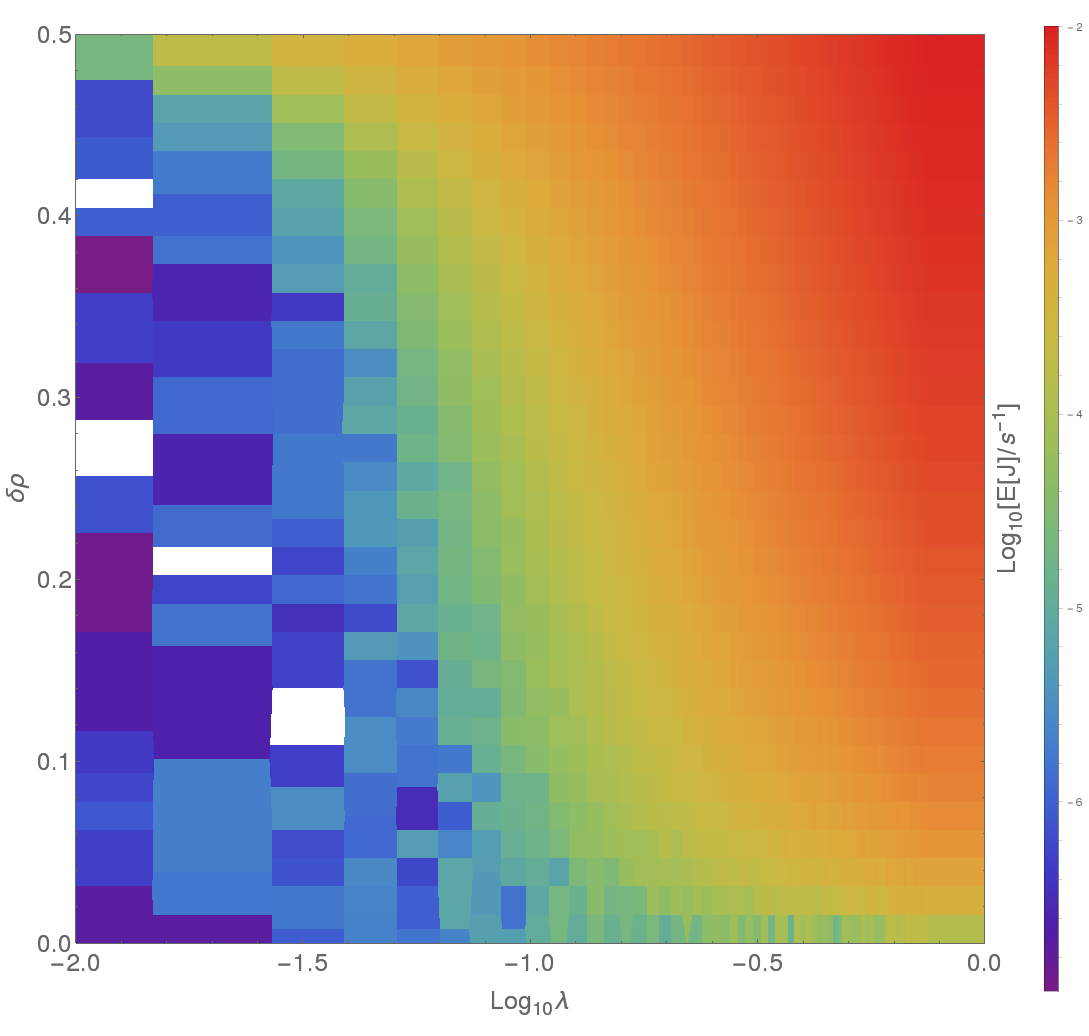
\includegraphics[width=0.49\linewidth]{numerics/images/lambdaConcDiff/current} & 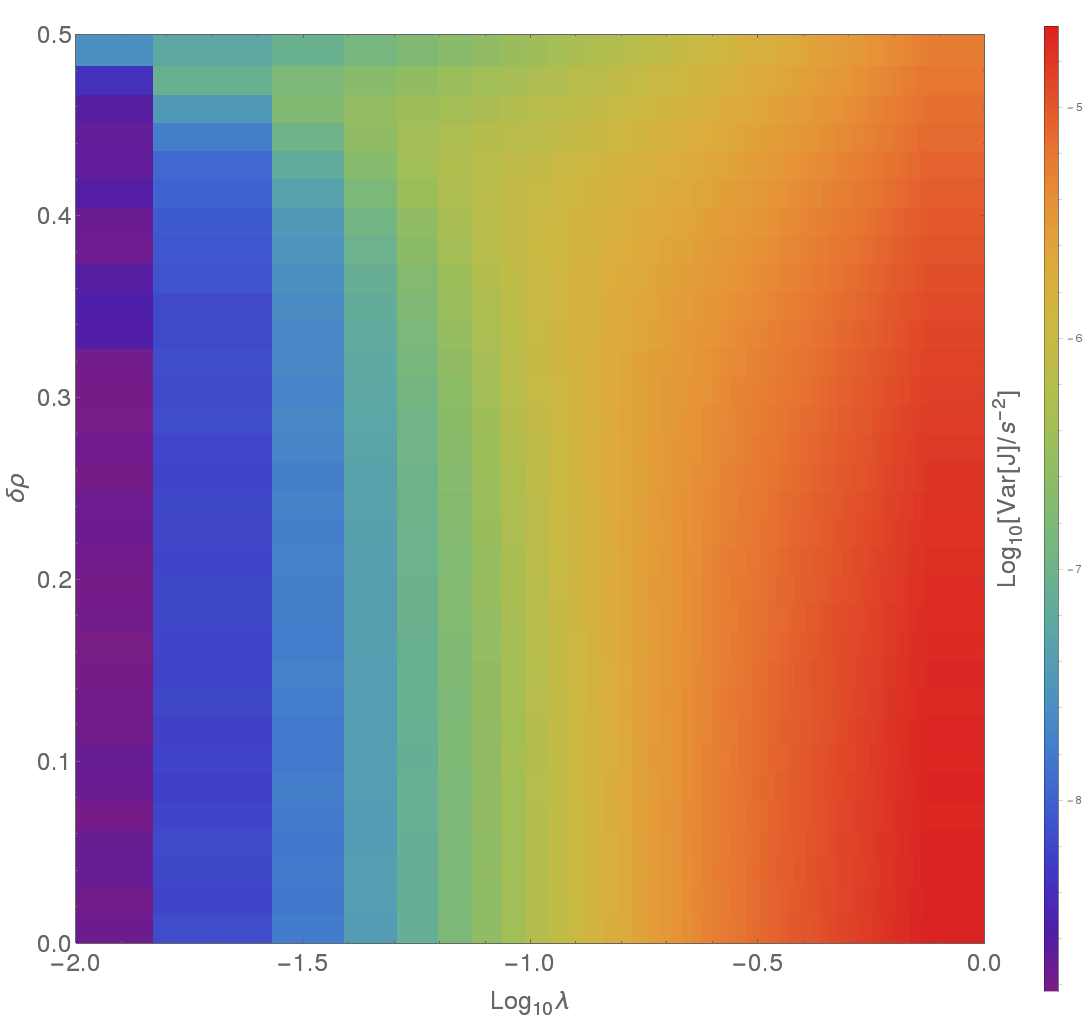
\includegraphics[width=0.49\linewidth]{numerics/images/lambdaConcDiff/currentVar} \\
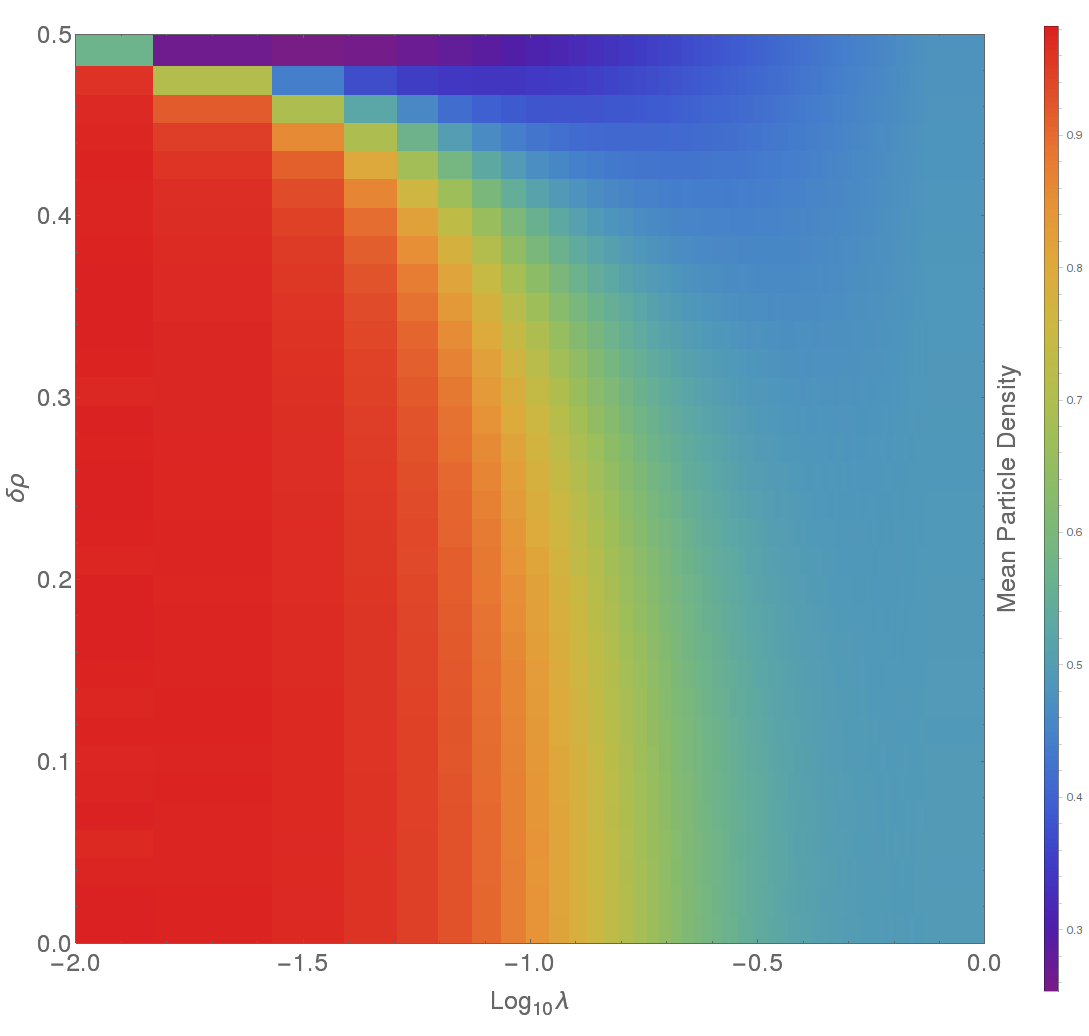
\includegraphics[width=0.49\linewidth]{numerics/images/lambdaConcDiff/density} &
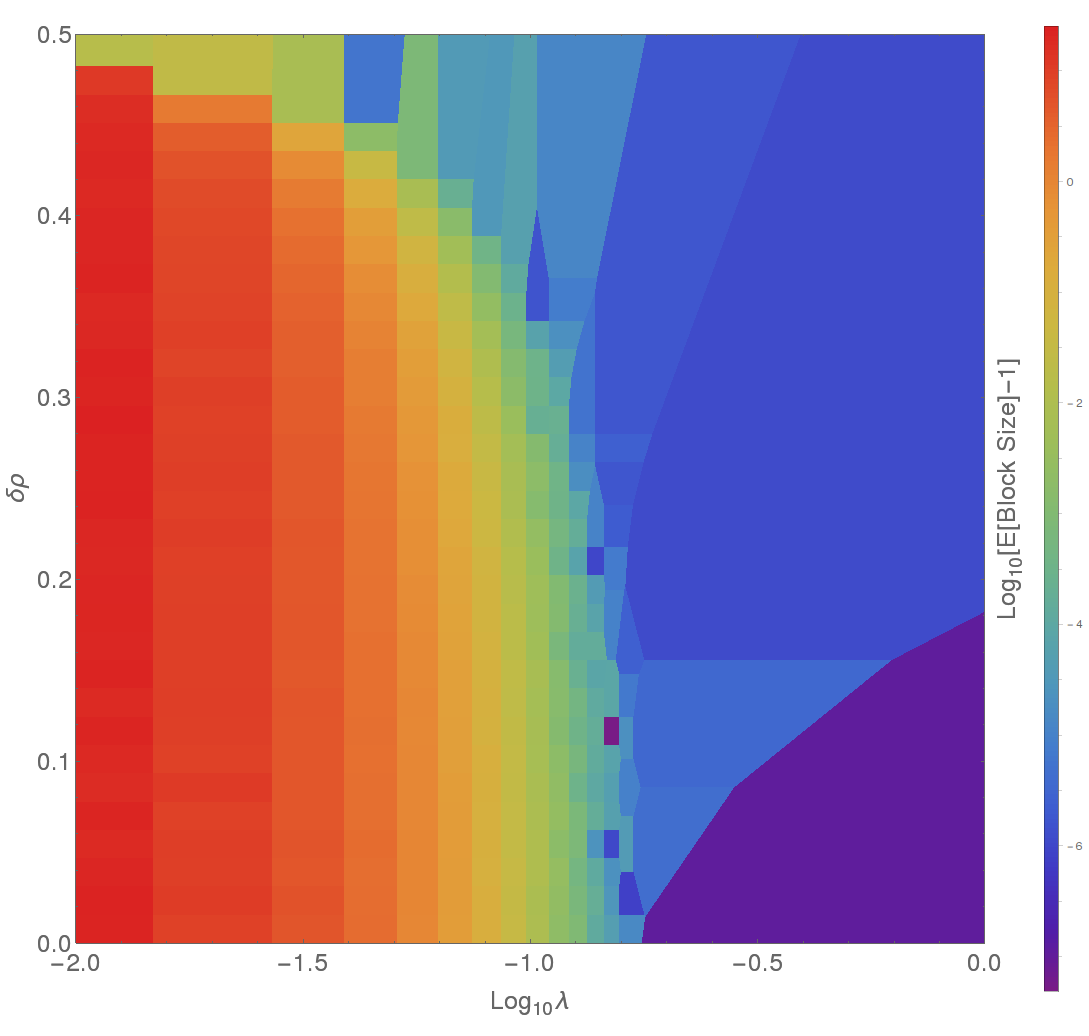
\includegraphics[width=0.49\linewidth]{numerics/images/lambdaConcDiff/blockSize} \\
\end{tabular}
\end{center}
\end{figure}

In each of these results, we see that we essentially partition the domain into two regimes:
small $\lambda$ with small $\delta \rho$, and another regime where $\lambda$ is larger, or 
$\delta \rho$ is bigger. In other words, when $\lambda$ becomes small the system gains density,
block size, and flow slows; however, a large boundary difference can still force through current
and keep density and block size lower, so there is a tradeoff between these competing forces.
\subsection{Varying the Boundary Densities with Constant $\lambda$}
Instead of varying $\lambda$, we can instead choose to hold it constant whilst we vary the two
boundary densities. We have done this with a series of different $\lambda$; the mean current results
are displayed in Fig.~\ref{fig:boundaryVarCurr}, and the mean densities displayed in 
Fig.~\ref{fig:boundaryVarDens}. Here we used $L=124$, with $160000000$ equilibration steps and then
$1000$ sets of analysis runs of $1600000$ KMC steps interspersed with relaxation runs of 
$1000$ steps.
\begin{figure} \caption[Mean currents observed when varying the boundary densities, fixing $\lambda$,
for different $\lambda$]{Here we have varied $\rho_0$ and $\rho_L$ separately for several different 
values of $\lambda$, and measured the resulting mean current. Note that here we have plotted the 
absolute value of the current, as it should be antisymmetric about $\rho_0 = \rho_L$, which would
not take kindly to having its logarithm taken.} 
\label{fig:boundaryVarCurr}
\begin{center}
\begin{tabular}{c c} 
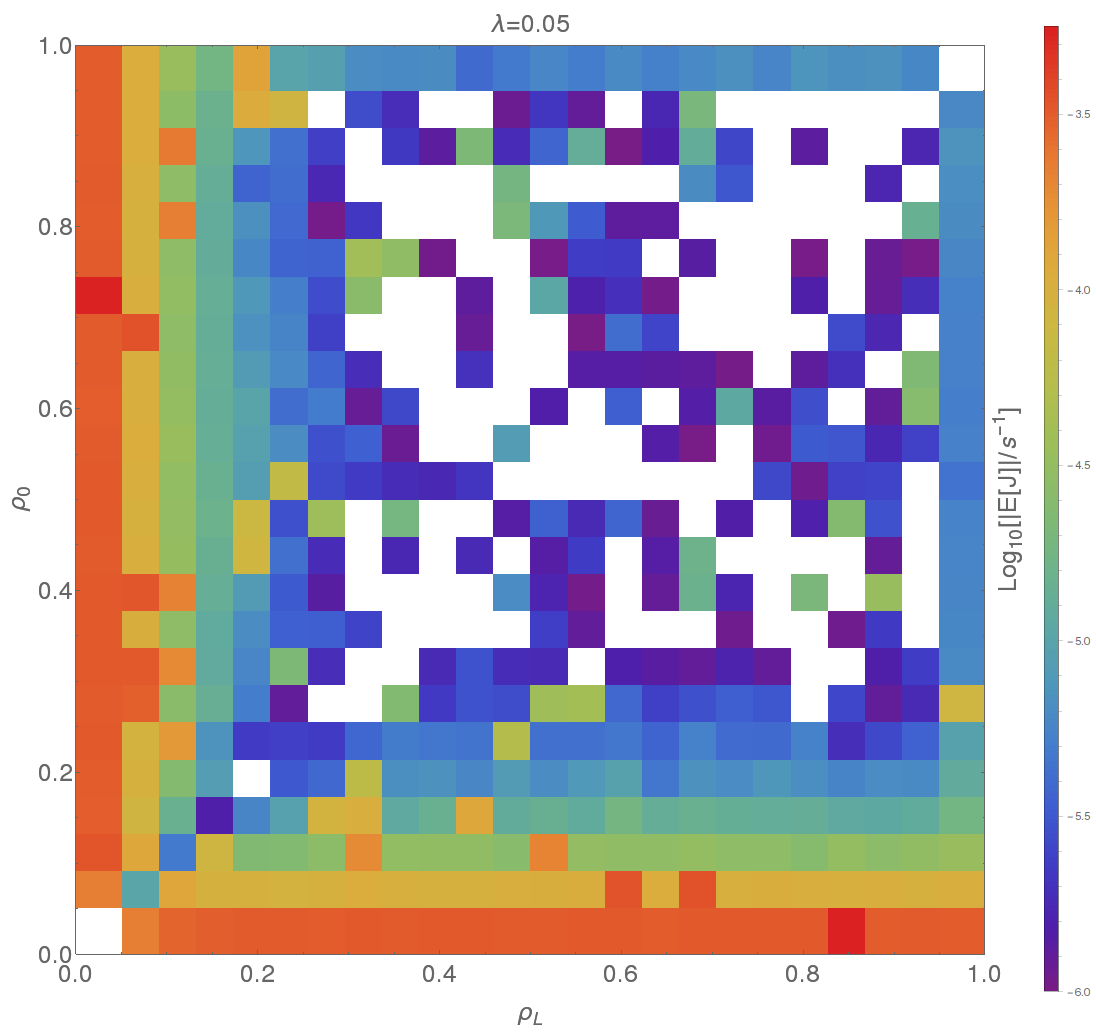
\includegraphics[width=0.49\linewidth]{numerics/images/concFrames/concDataCurr0p05.png} &
\includegraphics[width=0.49\linewidth]{numerics/images/concFrames/concDataCurr0p09.png} \\
\includegraphics[width=0.49\linewidth]{numerics/images/concFrames/concDataCurr0p13.png} & 
\includegraphics[width=0.49\linewidth]{numerics/images/concFrames/concDataCurr0p17.png} \\
\includegraphics[width=0.49\linewidth]{numerics/images/concFrames/concDataCurr0p21.png} &
\includegraphics[width=0.49\linewidth]{numerics/images/concFrames/concDataCurr0p25.png} \\
\end{tabular}
\end{center}
\end{figure}
\begin{figure} \caption[Mean densities observed when varying the boundary densities, fixing $\lambda$,
for different $\lambda$]{As Fig.~\ref{fig:boundaryVarCurr}, only this time we have plotted the mean 
densities instead of the currents.} 
\label{fig:boundaryVarDens}
\begin{center}
\begin{tabular}{c c} 
\includegraphics[width=0.49\linewidth]{numerics/images/concFrames/concDataDens0p05.png} &
\includegraphics[width=0.49\linewidth]{numerics/images/concFrames/concDataDens0p09.png} \\
\includegraphics[width=0.49\linewidth]{numerics/images/concFrames/concDataDens0p13.png} & 
\includegraphics[width=0.49\linewidth]{numerics/images/concFrames/concDataDens0p17.png} \\
\includegraphics[width=0.49\linewidth]{numerics/images/concFrames/concDataDens0p21.png} &
\includegraphics[width=0.49\linewidth]{numerics/images/concFrames/concDataDens0p25.png} \\
\end{tabular}
\end{center}
\end{figure}

We see a similar picture to the one we saw in Sec.~\ref{sec:constDens}; the system naturally 
wishes to relax to a high-density, low-current regime at small $\lambda$ regardless of boundary 
conditions, (probably primarily due to attempts to minimise free energy), but this is suppressed by
large boundary density differences.

\subsection{Diffusion Coefficient}
Wrapping up our calculations in $1$D, we can compute the effective diffusion coefficient, which
can be compared with our existing calculation in Sec.~\ref{sec:TRMDensityCurrent} (see 
Fig.~\ref{fig:TRMDiffCoeff} specifically for graphical comparison). To do this, we perform
calculations with boundary densities $(\rho_0, \rho_L)=(\rho + \frac{1}{2} \delta \rho , \rho -
\frac{1}{2} \delta \rho)$, where we vary $\rho$, $\lambda$ and $\delta \rho$ simultaneously, and
we deliberately keep $\delta \rho$ small, in the hope that the dependency of the current upon $\delta
\rho$ is roughly linear in that regime, so that $J = \frac{\delta \rho}{L} D(\rho, \lambda)
+ \mathcal{O}(\delta \rho^2)$. Given that we have an error estimate for $J$ due to repeat runs,
we can use weighted least squares fitting to estimate the value of $D(\rho, \lambda)$, and also
its error. We did this, using $16$ values of $\delta \rho$ for each $(\rho, \lambda)$ pair we
computed (arranged in a $24 \times 12$ grid); each computation consisted of a $160000000$ KMC step
equilibration run, followed by $10$ alternating $80000000$ step measurement run and $16000000$ step
relaxation run pairs. The system size used in this case was $L=124$. Our estimate for $D$ and its
standard error are displayed in
Fig.~\ref{fig:KMCDiffCoeff}.
\begin{figure} \caption[The variation of the KMC-calculated diffusion coefficient with $\rho$ and 
$\lambda$.]{The variation of the KMC-calculated diffusion coefficient with $\rho$ and 
$\lambda$. The top panel is the estimate of $D(\rho, \lambda)$, and the bottom panel is the associated
standard error.} 
\label{fig:KMCDiffCoeff}
\begin{center}
\begin{tabular}{c}
\includegraphics[width=0.95\textwidth]{numerics/images/diffCoeff/numDiffCoeff} \\
\includegraphics[width=0.95\textwidth]{numerics/images/diffCoeff/newFlowErr} \\
\end{tabular}
\end{center}
\end{figure}

Please note that whilst this is probably the largest single calculation we have performed during the 
course of this research, it is also the earliest chronologically; thus, there are many issues
with it:
\begin{itemize}
 \item We probably used a system that was unnecessarily large. A size $64$ system proved to be quite adequate
 later on, and equilibrates much faster.
 \item We should have performed a larger number of shorter analysis runs; that way we would
 probably obtain a more robust estimate for $D$, which wouldn't be so susceptible to being
 kicked around by individual rogue measurements.
 \item We only hit upon the idea of scanning in $\log \lambda$ instead of $\lambda$ later on
 in the research; thus, the format here does not allow for easy direct comparison with our TRM
 results which do use $\log \lambda$. 
\end{itemize}
That said, these results do compare nicely with our MFT calculations, displayed in 
Fig.~\ref{fig:diffCoeffDensityPlot}. The qualitative features are very similar, although the
MFT-predicted ``transition'' doesn't occur quite where it suggests, which we have seen  
more clearly in our scans in Sec.~\ref{sec:lambdaScans}.

\section{2D Calculation Results}
As we saw in Sec.~\ref{sec:highDimSPM}, it is possible to define a logical extension of the SPM
to dimensions higher than $1$D. Whilst it is not viable to perform TRM calculations in higher 
dimensions (as the scaling with system size is already very bad), it is relatively easy to adapt
our $1$D KMC codes to perform SPM calculations in $2$D or $3$D. Such a KMC input script may be found
here<insert code>. One thing that does need considering in this case is that a 2-dimensional square
lattice-based domain would normally have $4$ boundaries instead of $2$, which would mean $2$ extra
boundary conditions which would need to be prescribed in addition to $\rho_0$ and $\rho_L$.
However, we have avoided this difficult by making one of the coordinates cyclic; therefore, in our
$2$D calculations we are really considering flow down a tube, with circumference $W$. We still
use the same double-layered boundary technique as in $1$D, thus for a system of length $L$
we have $W \times (L+4)$ lattice sites in play.

\subsection{Aspect Ratio Considerations} \label{sec:aspectRatio}
Given that we now have two system size variables to play with, a natural question to ask would be
how the system's behaviour changes as we adjust $W$ and $L$, and in particular their aspect ratio.
We would expect that total current with given boundary conditions would usually scale inversely with
$L$ and in proportion to $W$ (as more current can flow across a wider cyclic surface); thus, the
total current should scale as $\frac{W}{L}$, the aspect ratio of the system. We can test this, and
also check how system convergence scales with system size, by performing calculations of the current
with several different $(L, W)$ pairs. We have maintained the boundary conditions to be 
$(\rho_0, \rho_L) = (0.75, 0.25)$ throughout, and in each case used an initial equilibration run of
$1600000$
KMC steps followed by $4096$ runs consisting of alternating $16000$-step and $320000$-step
analysis and relaxation runs respectively; then, we have varied $\lambda$ and measured the mean
current. The results are displayed in Fig~\ref{fig:aspectRatios}.
\begin{figure} \caption[The variation of the current in a $2$D SPM system with $\lambda$,
for a variety of different system sizes and aspect ratios.]{The variation of the current in a $2$D SPM
system with $\lambda$, for a variety of different system sizes and aspect ratios. The dotted
line indicates the relevant MFT prediction.} 
\label{fig:aspectRatios}
\begin{center}
\includegraphics[width=0.95\textheight, angle=270]{numerics/images/2d/sizeCompLambdaScan}
\end{center}
\end{figure}

Firstly, note that our supposition about the aspect ratio does appear to be true; the
data points for which the aspect ratio is $1$ line up quite nicely, and the situations
where it is $\frac{1}{2}$ or $2$ yield currents which are halved or doubled accordingly.
Notice also that the MFT prediction, whilst overestimating the actual $\lambda$ for 
which the transition occurs, is actually much better reproduced here than in $1$D, as here the
currents do indeed crash to zero much more clearly, in line with the idea that there should be a 
hard transition. It is also worth noting that the spread of the data, generally indicative
of both convergence quality as well as the actual current fluctuation, is very large for the 
larger system sizes. Thus, we can conclude that it is probably pointless trying to measure with
system sizes of $32\times 32$ or higher, as we just cannot achieve the calculational stability
required to say anything of consequence. On the other hand, whilst the system of size $8 \times 8$
gives nicely grouped data, it is also conceptually probably too small to be useful
to us (after all, in $1$D we can perform TRM calculations with length $8$). Thus, in our
next batch of calculations we decided to use systems of size $16 \times 16$.

\subsection{Varying $\lambda$ with Constant Boundary Conditions} \label{sec:2dLambdaScans}
We intended to perform a systematic battery of calculations in $2$D just as we have done in $1$D.
However, due to the bigger issues with equilibration and overall computational time which occur in $2$D we found that performing decent calculations was much more difficult than we anticipated; thus, due to time constraints, we only managed to perform one high-quality calculation.
This is a scan through values of $\lambda$ with fixed boundary conditions, similar to our work
in Sec.~\ref{sec:lambdaScans}. Here we used $L \times W = 16 \times 16$, allowed $16000000$ KMC
steps for equilibration time, and then did $4096$ measurement cycles of alternating $16000$-step
and $320000$-step analysis and relaxation runs, just like in Sec.\ref{sec:aspectRatio}.
Our results for the overall system density are displayed in Fig.\ref{fig:2dSysDens}, and
our measurements of current and its variance are shown in Fig.\ref{fig:2dSysCurr}.
\begin{figure} \caption[The variation of the overall density in a $2$D SPM system with 
$\lambda$.]{The variation of the overall density in a $2$D SPM system with $\lambda$, with
$3$ sets of boundary conditions as indicated.} 
\label{fig:2dSysDens}
\begin{center}
\includegraphics[width=0.95\textheight, angle=270]{numerics/images/2d/2dDensity}
\end{center}
\end{figure}
\begin{figure} \caption[The variation of the mean current and its variance in a $2$D SPM system
with $\lambda$.]{The variation of the mean current and its variance in a $2$D SPM system
with $\lambda$, with boundary conditions as indicated. The mean current is the top panel,
and the current variance is the bottom panel.} 
\label{fig:2dSysCurr}
\begin{center}
\begin{tabular}{c}
\includegraphics[width=0.95\textwidth]{numerics/images/2d/2dCurrentMeans} \\
\includegraphics[width=0.95\textwidth]{numerics/images/2d/2dCurrentVars} \\
\end{tabular}
\end{center}
\end{figure}

Let us discuss the density results first, as without those the current results don't make as
much sense. The density changes with $\lambda$ are similar to our $1$D results in the sense
that the density attempts to converge to $1$ for extremely small values of $\lambda$ regardless
of the actual boundary conditions used, and the density has an inflection or minimum in each case for some
$\lambda$ a little below $1$.

However, there are some big differences:
\begin{itemize}
 \item The density does \textbf{not} appear to be converging to some common value regardless of
 boundaries in the large-$\lambda$ regime like it did in $1$D. A possible explanation for this
 is that there is not a straightforward family of bulk maximal-flow configurations which are
 inherently more stable than their rivals like there seems to be in $1$D; instead, due to the
 larger space of possible configurations available in $2$D, it may be the case that there are many
 different ways of realising fast rapid flow, which have different densities. An easy way to test
 this would be to perform similar calculations to these, but with a greater variety of boundary
 conditions; then, one should be able to observe whether the spectrum of densities in
 the large-$\lambda$ (repulsive) limit is continuous or discrete.
 \item For our low-density choice of boundary conditions $(\rho_0, \rho_L) = (0.3, 0.1)$,
 it would appear that the mean overall system density splits into two separate branches,
 forming a curve reminiscent of the hysteresis curves exhibited by ferromagnets <ref>. This
 is perhaps not so surprising, as there is a relationship between the $2$D SPM and the $2$D Ising
 Model with fixed magnetisation. Our interpretation of this is that in this regime there are
 two flow-permitting configurations which both satisfy the desired boundary conditions
 and are both fairly stable, at least over the timescale of our measurements. Looking at it in 
 this way, this appears to be another example which illustrates the possibility that there can
 be competing stable/metastable states in $2$D which cannot occur in $1$D because there is
 insufficient freedom.
\end{itemize}
So far as the current is concerned, we see broadly the same behaviour as in our (linear) plot
in Fig~\ref{fig:aspectRatios}; the current has roughly power-law dependence on $\lambda$ for
large $\lambda$, partially agreeing with the MFT prediction, before dissolving into noise
below a threshold in $\lambda$. The mean current for our low density boundary choice exhibits branching just
like
the density does, suggesting that the effective diffusion coefficients of the competing 
configurations are different. The current variance is broadly power-law with $\lambda$,
with kinks around the transitions and again some exhibition of the ``hysteresis''-like branching.

Another way to look at this branching is to consider the fact that researchers have observed 
``stripes'' in the KLS model <ref>. In that particular context the model contains asymmetric
bulk dynamics, and stripes of low and high density spontaneously form and spiral around the 
system, transmitting current as they do so. It could be the case that our $16 \times 16$ system
tries to generate such stripes, but is too small to support more than one stripe; thus, instead
different stripes are realised in different simulations. Of course, as this system is ergodic, we
should in the long-term limit see both stripe types manifest in any given simulation; however,
the switching time, if both stripe types are quite stable, might be so long that we would never
actually observe this happening.

\section{Conclusions}
The primary conclusions from our work with Monte-Carlo methods is as follows:
\begin{itemize}
 \item Our Monte-Carlo work with $1$D systems yields results very similar to those we 
 have already observed using our Transition-Rate Matrix method; thus, our fears that the small
 systems we investigated using TRM were too small to properly portray the properties of larger
 systems seem to have gone unrealised.
 \item These results appear to confirm our observation that a \textit{power law 
 switching} phenomenon does indeed occur in $1$D. Likewise they support our hypothesis that
 $1$D systems with large $\lambda$ self-organise to yield similar system configurations
 regarless of boundary conditions, in an effort to maximise flow (or more directly, system
 stability).
 \item Our foray in $2$D has been brief, but suggests that there is much more interesting material to study there, in particular the limiting behaviours with extreme $\lambda$
 and the hysteresis-curve effect we see in the density for low-density boundary configurations.
\end{itemize}






To conclude, we have solved a nonlinear model for self-interacting sticky particles diffusing in 1D.  Although only the particles exhibit stickiness,  the analytics suggest a symmetry between vacancy-type and particle-type flow
at density of $\frac{2}{3}$, which is observed in the simulation.  The flow exhibits a foamy pattern with intermediate time-and-space correlations.  The continuum solution MFT is a good predictor of the bulk flow behavior of the SPM.
The negative diffusion constant found in MFT at high stickiness indicates  that the assumption of homogeneous density break down: thus the MFT predicts its own demise.

We would like to thank EPSRC (student grant 1527137) and Wolfson Foundation for providing the funding, Mikael Leetmaa for producing \texttt{KMCLib}, and the \texttt{Eddie3} team here at Edinburgh for maintaining the hardware used.
We would also like to thank Martin Evans, Bartek Waclaw and Richard Blythe for some very helpful discussions during the production of this letter.
% Need to say something like `` See Supplemental Material at [URL will be inserted by publisher] for [give brief description of material]. ''

\appendix
\addtocontents{toc}{\protect\tocappendix}
\chapter{Code Listings}

\section{1d Ising Correlation Functions \label{sec:corrFnCode} }

This \texttt{Python} script computes the probability of a site being occupied $l$ lattice spacings away from an occupied site.
It requires the system size $L$ and the number of particles $N$ as inputs. The output is saved in a file called \texttt{corrFnResults.m}, which is formatted so that it may be used by \texttt{Mathematica}.

\begin{lstlisting}[language=Python]
import copy
import sys

def configMake(L, N, prevList, totList):
    if L==1:
        endList = [copy.deepcopy(prevList), N]
        totList.append(unfold(endList))
        return [N]
    if N==0:
       return configMake(L-1, 0, [copy.deepcopy(prevList), 0], totList)
    if L==N:
        return configMake(L-1, N-1, [copy.deepcopy(prevList), 1], totList)
    return [configMake(L-1, N, [copy.deepcopy(prevList), 0], totList),
    configMake(L-1, N-1, [copy.deepcopy(prevList), 1], totList)]

def adjSum(candList):
    listLen = len(candList)
    total = 0
    for index in range(0, listLen):
        total += candList[index-1]*candList[index]
    return total

def unfold(candList):
    if isinstance(candList, list):
        if len(candList)==2:
            return unfold(candList[0])+unfold(candList[1])
        if len(candList)==1:
            return candList
        if len(candList)==0:
            return []
    return [candList]

def listCollate(candList):
    maxItem = 0
    for index in candList:
        if index > maxItem:
            maxItem = index
    outPut = []
    for size in range(0, maxItem+1):
        numCounts = 0
        for index in candList:
            if index == size:
                numCounts += 1
        outPut.append((size, numCounts))
    return outPut

def genCorrFn(L, N):
    totList = []
    allStates = configMake(L, N, [], totList)
    restStates = []
    weightList = []
    maxAdj = 0
    for state in totList:
        if state[0]==1:
            restStates.append((state, adjSum(state)))
            if restStates[-1][1]>maxAdj:
                maxAdj = restStates[-1][1]
            weightList.append(restStates[-1][1])
    partFnList = listCollate(weightList)
    print(partFnList)
    partitionFn = "("
    for pair in partFnList:
        partitionFn += str(pair[1])+" Exp["+str(pair[0]-maxAdj)+"b] + "
    partitionFn += "0)"
    print(partitionFn)
    finalOut = "{"
    for shift in range(0, L-L/2):
        tempList = []
        for config in restStates:
            if config[0][shift] == 1:
                tempList.append(config[1])
        stateDist = listCollate(tempList)
        outSum = "{"+str(shift)+", ("
        for pair in stateDist:
            outSum += str(pair[1])+" Exp["+str(pair[0]-maxAdj)+"b] + "
        outSum += "0)/"+partitionFn+"}"
        finalOut += outSum
        if shift != L-L/2-1:
            finalOut += ", "
    finalOut+="}"
    return finalOut

L = int(sys.argv[1])

with open("corrFnResults.m", 'w') as f:
    f.write("{")
    for n in range(2, L-2):
        f.write("{"+str(n)+"/"+str(L)+", "+genCorrFn(L, n)+"}, ")
    f.write(genCorrFn(L, L-2) + "}")
\end{lstlisting}

\section{$n$-Dimensional Continuum-Limit MFT \label{sec:mftCode}}

This Mathematica script computes the current which flows between two adjacent sites
(offset in the $e_1$ direction) in the MFT of the $n$-dimensional SPM; due to symmetry, this tells us
what happens in an arbitrary direction. In this case $n$ is set to $3$,
but it still works if changed to any positive number.

\begin{lstlisting}[language=Mathematica]
n = 3;
i = 1;
zero = 0*UnitVector[n, 1];
e[i_] := UnitVector[n, i];
Hess = Table[
   Piecewise[{{d2p[j, i], j > i}}, d2p[i, j]], {i, 1, n}, {j, 1, n}];
Jacob = Table[dp[i], {i, 1, n}];
p[x_] := p0 + Jacob.x + 1/2 x.(Hess.x);
rightJ = 1/
    t0 (1 - p[1/2 a e[i]]) p[-(1/2) a e[i]] (1 - 
     z p[-(3/2) a e[i]]) Product[
    Piecewise[{{(1 - z p[-a e[j] - 1/2 a e[i]]) (1 - 
          z p[a e[j] - 1/2 a e[i]]), j != i}}, 1], {j, 1, n}];
leftJ = 1/t0 (1 - p[-(1/2) a e[i]]) p[
    1/2 a e[i]] (1 - z p[3/2 a e[i]]) Product[
    Piecewise[{{(1 - z p[-a e[j] + 1/2 a e[i]]) (1 - 
          z p[a e[j] + 1/2 a e[i]]), j != i}}, 1], {j, 1, n}];
fullJ = rightJ - leftJ + O[a]^3;
FullSimplify[fullJ]
\end{lstlisting}




\backmatter

\singlespace

\phantomsection
\addcontentsline{toc}{chapter}{\bibname}
% Choose a bibliography style to suit your taste here
% This one was downloaded from http://web.reed.edu/cis/help/latex/bibtexstyles.html (June 2012)
\bibliographystyle{ChicagoReedweb}
\bibliography{overallBib}

\end{document}
